\documentclass[12pt, a4paper, UKenglish, final]{report}
\usepackage[utf8]{inputenc}
\usepackage{amsmath}
%\usepackage{mathtools,amssymb}
\usepackage{algorithm2e}
%\usepackage[noend]{algpseudocode}
\usepackage{babel,csquotes}
\usepackage{float}
\usepackage{ifimasterforside}
\usepackage{listings}
\usepackage{wrapfig}
\usepackage{graphicx}
\usepackage{fancyhdr}
\usepackage[backend=biber,
	    style=numeric,
	    citestyle=numeric]{biblatex}

\addbibresource{references.bib}


\usepackage{xcolor}
\usepackage{wrapfig}
\usepackage{caption}
\usepackage{subcaption}
\pagestyle{fancy}
\fancyhead{}
\fancyhead[RO,LE]{\leftmark }
\fancyfoot{}
\fancyfoot[CO,RE]{\thepage}

\makeatletter

\newcommand\frontmatter{%
	\cleardoublepage
	%\@mainmatterfalse
  \pagenumbering{roman}}

\newcommand\mainmatter{%
	\cleardoublepage
	% \@mainmattertrue
  \pagenumbering{arabic}}

\newcommand\backmatter{%
	\if@openright
    \cleardoublepage
  \else
    \clearpage
  \fi
  % \@mainmatterfalse
   }

\DeclareFixedFont{\ttb}{T1}{txtt}{bx}{n}{11} % for bold
\DeclareFixedFont{\ttm}{T1}{txtt}{m}{n}{11}  % for normal

% Custom colors
\usepackage{color}
\definecolor{deepblue}{rgb}{0,0,0.5}
\definecolor{deepred}{rgb}{0.6,0,0}
\definecolor{deepgreen}{rgb}{0,0.5,0}

\usepackage{listings}

% Python style for highlighting
\newcommand\pythonstyle{\lstset{
language=Python,
stepnumber=1, 
breaklines=true,
basicstyle=\scriptsize\ttfamily,
otherkeywords={self},             % Add keywords here
keywordstyle=\scriptsize\ttfamily\color{deepblue},
emph={MyClass,__init__},          % Custom highlighting
emphstyle=\ttb\color{deepred},    % Custom highlighting style
stringstyle=\color{deepgreen},
frame=tb,                         % Any extra options here
showstringspaces=false            % 
}}


% Python environment
\lstnewenvironment{python}[1][]
{
	\pythonstyle
\lstset{#1}
}
{}

% Python for external files
\newcommand\pythonexternal[2][]{{
	\pythonstyle
\lstinputlisting[#1]{#2}}}

% Python for inline
\newcommand\pythoninline[1]{{\pythonstyle\lstinline!#1!}}
\makeatother
\colorlet{punct}{red!60!black}
\definecolor{background}{HTML}{EEEEEE}
\definecolor{delim}{RGB}{20,105,176}
\colorlet{numb}{magenta!60!black}

\lstdefinelanguage{json}{
	basicstyle=\scriptsize\ttfamily,
    numbers=left,
    numberstyle=\scriptsize,
    stepnumber=1,
    numbersep=2pt,
    showstringspaces=false,
    breaklines=true,
    backgroundcolor=\color{background},
    literate=
     *{0}{{{\color{numb}0}}}{1}
      {1}{{{\color{numb}1}}}{1}
      {2}{{{\color{numb}2}}}{1}
      {3}{{{\color{numb}3}}}{1}
      {4}{{{\color{numb}4}}}{1}
      {5}{{{\color{numb}5}}}{1}
      {6}{{{\color{numb}6}}}{1}
      {7}{{{\color{numb}7}}}{1}
      {8}{{{\color{numb}8}}}{1}
      {9}{{{\color{numb}9}}}{1}
      {:}{{{\color{punct}{:}}}}{1}
      {,}{{{\color{punct}{,}}}}{1}
      {\{}{{{\color{delim}{\{}}}}{1}
      {\}}{{{\color{delim}{\}}}}}{1}
      {[}{{{\color{delim}{[}}}}{1}
      {]}{{{\color{delim}{]}}}}{1},
}

\title{Group creation in a collaborative P2P channel allocation protocol}
\subtitle{Identifying connected groups of access points}
\author{Hans Jørgen Furre Nygårdshaug}

\begin{document}
\ififorside
\maketitle{}
\frontmatter

\section*{Abstract}
\clearpage
%\section*{List of acronyms}
%\begin{tabular}{ c c }
	%\textbf{AP} & Access Point\\ 
	%\textbf{CSMA/CA} & Carrier Sense Multiple Access / Collision Avoidance\\
	%\textbf{MAC} & Medium Access Control\\
	%\textbf{CCA} & Clear Channel Assessment\\
	%\textbf{MAC} & Mandatory Access Control\\
	%\textbf{PHY} & Physical Layer\\
	%\textbf{PLCP} & Physical Layer Convergence Procedure\\
	%\textbf{PPDU} & PLCP Protocol Data Unit\\
%\end{tabular}
\tableofcontents
\listoffigures

\mainmatter
\chapter{Introduction}
The presence of Internet connected devices is still rapidly expanding. The latest forecast 
esitmates that there will be about 27 billion devices connected to the Internet by 2021 \cite{CiscoVNI2017}, while by the end of the 2017 the number
connected devices in use will be 8.4 billion \cite{Gartner}. In 2020 households alone will be responsible for over 10 billion devices that are
able to wirelessly connect to the home router \cite{wifialliance}, and wireless traffic will account for 63 percent of all IP traffic in the world \cite{CiscoVNI2017}. 
Traditionally devices that are commonly connected to the Internet in a household are computers, phones, watches, smart TVs, audio systems, and lately also private network storage systems.
As the era of Internet of Things (IoT) has rapidly descended upon us, increasingly also less obvious utilites are connected to the Internet.
These devices may span everything from lights and HVAC systems to coffee machines, fridges and even toasters. Whereas in the early 2000s it was common to own 
one or two MAC-addresses per person, at the date of writing it is not unusual to possess a two digit number of MAC-addresses.

But it is not only the numbers of devices that has changed. The consumers' expectations and demands are also being altered over time. 
While ubiquitous connectivity is a buzzword often heard in the context of future 5G networks, ubiquitous access is already expected in
modern households. The demand for Wi-Fi coverage extends through the entire home: the Internet radio in the garage, the video stream on the basement
couch and the gaming laptop on the bedroom. All demands coverage and expects mobility at the same time. These devices also have something else in
common that reflects the change that has happened the last years: demand for high data rate. In 2016 about 73 percent of all IP traffic orginated from video
streams, and in 2021 this number is expected to increase all the way up to 82 percent \cite{CiscoVNI2017}. 

This demand for continous streams of high bitrate video poses a challenge that can not only be solved by providing larger bandwidth. First of all, video streams
have high Quality of Service (QoS) demands. Buffering of videos and reduction of video quality negatively affects the subjective experience.
Secondly, it is not unusual that different video flows occur simultaneously in a single residence. If such traffic is transmitted wirelessly
it results in an inherently busy transmission medium. Because of the international spectrum allocation standards, Wi-Fi is largely restricted to a small number of channels.
To overcome this challenge, the 802.11 protocol specifies a set of rules which allows only one device in the vicinity to transmit on a channel at the same time. 
This poses yet another challenge of distributing channels in a way that as few devices on the same channels as possible are close to one another. 

In short, while the physical layer (PHY) traditionally has been upgraded to meet the new demands in bitrate (e.g. fiber to the home, 
and MIMO in 802.11ac) Wireless LAN connections struggle under the heavy impact of RF-intereference which can not be solved by increasing
the physical datarate capacity. 

\section{Motivation}
Wireless LAN is deployed in almost all corporate buildings and residencies in the western world and increasingly also in the rest of the world.
The use of these networks used to be limited to laptops that generated small amounts of data, but now the range of devices includes
smart-phones, network storage devices, even in some cases servers. The deployment of Wi-Fi and the infrastructure has not 
changed much over the years to match the new demands and increased traffic, and in most places coverage is still the main concern, while
QoS comes second. 

Customers who are subscribed to high data rate service level agreements often find they can only receive a comparable data rate over wired LAN.
When the Wi-Fi network in their home is constantly underperforming, it is not unusual a customer to upgrade the data rate of their agreement. Often interfering networks
are the perpatrators, and an increase of bandwith will have no effect. This can lead customers to frustration with their Internet service providers,
even though it is the underlying technology, and not the service provider which is at fault.

A customer service representative or a tech-savvy consumer may manually switch the operating channel for a wireless access point.
If this has no effect a customer might be encouraged to get a router which can transmit a more powerful signal. While this might give a short relief
for the customer who was resourceful enough to deal with the problem, it in turn may trigger a chain reaction of even stronger
interference levels for the rest of the inhabitants in the surrounding area. 

There has been done research on how centralized controllers can benefit the deployment of large enterprise networks (\cite{Murty}, \cite{Murty2} and \cite{Suresh}),
but in this thesis we will address the emerging issue of deployment of Wi-Fi in residential areas and how routers and access points could organize themselves in self managing groups, 
to allow distributed control and coopeation on channel allocation, where centralized controllers are impractical or impossible.

\section{Problem definition}
There are 3 non-overlapping channels on the 2.4GHz spectrum that 802.11 Wireless LANs uses. One of the common ways of selecting a channel
is done by letting an access point sense which channel has the lowest interference levels, also called least congested channel search.
When channels are selected in a selfish manner, where the only available information about the surrounding networks are obtained via
subjective radio readings, it is highly unlikely that the distribution of channels in a confined area (e.g. an apartment block) becomes optimal.  
Ideally all the access points would be configured so that the channel distribution in this area lead to as few equal channels as possible
being adjacent to one another. While this boils down to a NP-complete graph-coloring problem, it is not the focus of this thesis.
The main challenge to be considered is the clustering problem of identifying access points that heavily impacts eachother, and consider different approaches to how 
they can form groups in a distributed manner that seeks to intuitively identify nodes that lie withing the same confined areas, as apartment buildings
dense residential areas, etc. 

\section{Method}
To be able to see if we can form groups in a way that creates clusters of nearby nodes we need to get some data to perform
calculation on. We will both create syntethic data and use real world location data of access points to evaluate the performance of the group creations. 
Then we will take a look at possible solutions to let access points communicate with each other without any manual bootstrapping or 
previous association. Then we will consider the problems and challenges that has to be overcome in the process of creating and deploying 
an architecture as suggested in the thesis. 

    %We will take a look on earlier algorithms in the research of finding a better way to allocate channels in 802.11. 
    %Then we can do a number of assumptions to be able to propose an algorithm for group creation amongst unorganized access points,
    %and then evaluate the algorithm by computing groups and clusters of access points.  




%\section{Channel allocation} 
%To deal with the problem of channel allocation we will think of an AP as a vertex in a graph. When an AP scans its radio
%it can hear the strength of all nearby wireless networks measured in dBm (decibel milliwatts). This decibel value will be
%the value of the edge between one AP to another. With a graph expressing the wireless network topology, the problem
%of optimally distributing channels between APs boils down to a graph coloring problem. The number of colors in the color problem,
   %represents the number of non-overlapping channels in 802.11. Exactly how an algorithm can be designed to optimally distribute channels within the
   %interfering topology is out of the scope of this thesis. However we can define some invariants that has to be true
   %for such an algorithm to work:
   %\begin{enumerate} 
   %\item All APs has to run the same algorithm
   %\item All APs must run the algorithm on the same connected group
   %\item Because of the complexity of the problem the algorthm must solve, the number of APs in the connected group can not be too big
   %\end{enumerate}
%
   %Point 1 is trivial to solve or mitigate, as only APs running the algorithm will actively participate in the channel selection. A simple way to make sure that the
   %same algorithm is used, is by having a software version that is consistently checked with the other APs in the connected group.
%
   %Point 2 and point 3 is will be the main focus of the rest of the master thesis, as these are not so easily solved.
%
   %We can define a wireless topology graph as a set of wireless APs that are grouped together and share information about their neighbours and interference levels.
   %This set is what will now on be referred to as a \textit{connected group.} All members of the connected group will be considered when running the channel assignment algorithm.
   %For the connected group to have an actual impact on the quality of a network connection, it has to consist of nodes that normally disturbs each other substantially.
%
   %An ideal example of a connected group is an apartment builiding. The channel allocation protocol lets APs share information about who-disturbs-who the most in the building.
   %Then each AP can run the channel allocation algorithm. Because they run it on the same graph, every AP will find the same optimal channel distribution throughout the building,
   %and then switch to the correct channel. 
%
   %Even though an apartment building is most likely an optimal delimination of a connected group, in reality creating such a group is a bigger challenge. As the whole channel allocation
   %protocol is based on decentralized peer-to-peer technology, and no centralized server with access to demographical and geographical divisions exists, the protocol will
   %have to discover suitable connected groups on its own. Moreover, when the group is created the protocol will have to replicate data so that
   %all participants of the group has all the data required to perform channel allocation. It will also need a way to make sure that the image of the current group
   %is consistent within all APs in the connected group. 



\chapter{Background}
In this chapter the relevant aspects of wireless technology and a selection of important
concepts from the 802.11 standard will be introduced.

\section{Basic radio challenges}
There are some challenges with wireless technologies that are harder to overcome when comparing to wired transmission technologies like Ethernet.

The first step to achieve a successful transmission is making sure the receiving radio is within transmit range of the transmitter. The
transmit range is decided by the power of which a signal is transmitted at, the antenna gain, and the surrounding 
environment. If there are a lot of solid obstacles, like walls and ceilings, the signal is likely to have a more compromised range.

Even if the surrounding environment is mostly open space, the wireless signal becomes subject of attenuation,
     which is a physical property of electromagnetic waves that weakens the signal the longer it has travelled through a
     medium. When this medium is only air, the phenomenon is referred to as free space path loss. Attentuation limits
     the transmit range of a radio, and to transmit further it has to increase its transmission power.

     \subsection{Collisions in wireless technology}
     Given two radio devices A and B, if there are any other nodes nearby that are within radio B's sensing range that sends at the same time as A, 
     radio B experiences radio frequency interference, and thus may not be able to correctly decode the signal of A. In 802.3 Ethernet this
     is graciously handled by collision detection in the CSMA/CD protocol. As each node can hear all other nodes on a wired medium,
     and listening while transmitting is generally not a problem, a node can retransmit if a collision is detected. In wireless techhnologies
     it is not equally easy to listen while transmitting, and collision detection may be impossible because of the hidden terminal problem.

     \subsubsection{The hidden terminal problem}
     The hidden terminal problem is one of the major challenges for wireless technologies, and a brief explanation of the problem will be offered here.
		 When node A transmits a message to node B, it may not be able to sense what is going on
     on the opposite side of node B. If a node C transmits at the same time, this signal may not enter node A's sensing range, and
     hence go undetected by, even though a collision has happened near node B. This is illustrated in figure \ref{fig:hiddenterminal} where
     both A and C has unknowingly sent messages at the same time, and B has not been able to decode either of the two, as they have been corrupted during
		 transmisison due to the collision. 

     \begin{figure}
     \center
		 \subfloat[A and C transmitting unknowingly at the same time, resulting in a collision at B]{{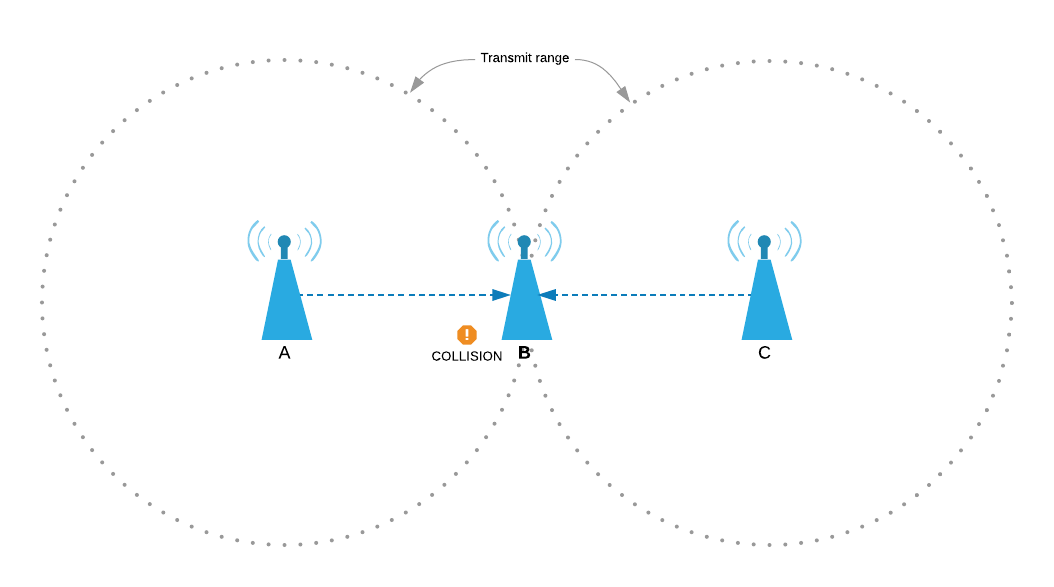
\includegraphics[width=13cm]{Images/HiddenTerminal.png} }}%

     \caption{The hidden terminal problem illustrated}
     \label{fig:hiddenterminal}
     \end{figure}


\section{Network infrastructure}
		This section provides a brief introduction to network infrastructures, to get an understanding of the differences between the mainly two types of infrastructures used today. 
		\subsection{Basic Service Set}
		A basic service set (BSS) in infrastruture mode consists of a single access point (AP) connected by wire to a distribution system (in residential deployment the distribution system is typically the ISP).
		Stations within the basic service area, which is the area physically serveable by the AP, can connect to the BSS using dynamic access point association, described
		in \cite{std80211}. A minimalist BSS infrastructure is illustrated in \ref{fig:basicserviceset}. It also worth mentioning that a BSS can also be configured to operate as an independent
		basic service set, where there is no infrastructure in place (no APs), and communication is direct between stations. This is more commonly known as ad-hoc mode.
		
		One basic service set per household is the typical infrastructure in residential networks, but it is not uncommon to have multiple basic service sets in larger homes,
		where APs are placed on different floors to have a better signal strength. Usually these APs have different service set identifiers (SSIDs), and each requires its own authentication.
		This is because the APs are not under the same extended service set. 

		 \begin{figure}
			 \center
			 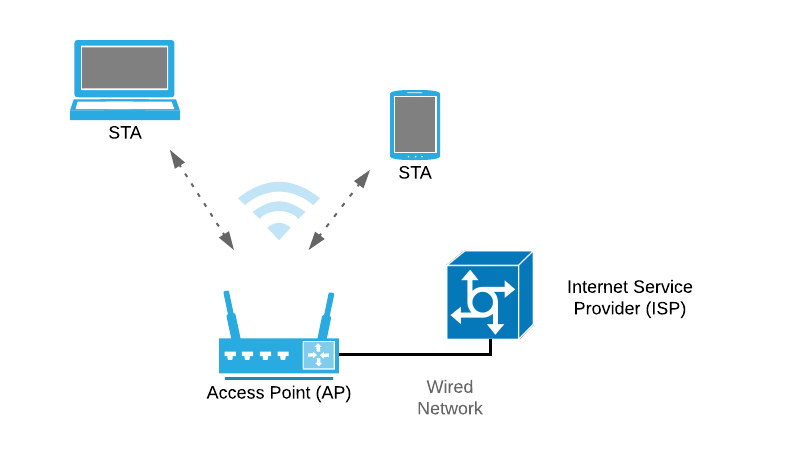
\includegraphics[scale=1]{Images/BSS.png}
			 \caption{Minimalist Basic Service Set in infrastructure mode}
			 \label{fig:basicserviceset}
		 \end{figure}

		\subsection{Extended Service Set}
		An extended service set (ESS) can consist of multiple basic service sets, and thereby APs. The extended service set is a logical entity which can extend station
		authentication and association to all APs under the same extended service set. In an ESS the SSID of all APs are also identical. This means a station (STA) can be in the basic service area of
		multiple APs at the same time, and is given the opportunity to select which AP to be serviced by. APs in an ESS can operate on different channels, and the medium access control
		mechanisms are performed as usual. Figure \ref{fig:extendedserviceset} illustrates the infrastructure of an extended service set.  

		 \begin{figure}
			 \center
			 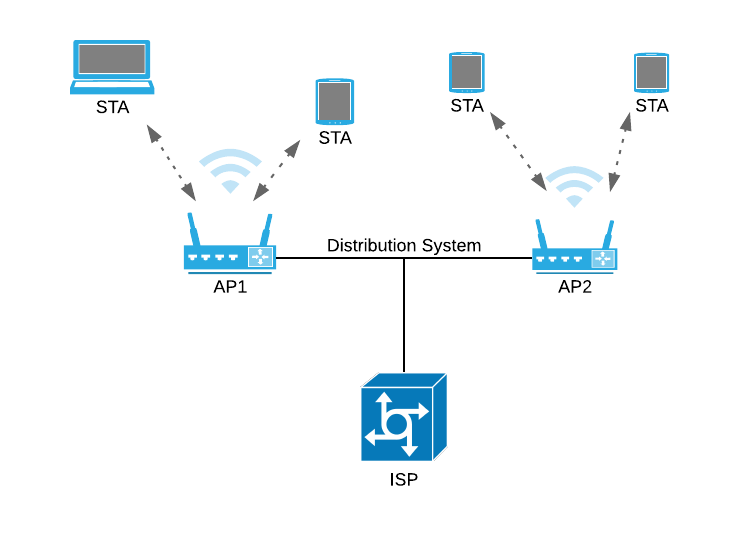
\includegraphics[scale=1]{Images/ESS.png}
			 \caption{Extended Service Set}
			 \label{fig:extendedserviceset}
		 \end{figure}


     \section{MAC Layer}
		 In this section parts of MAC layer of the 802.11 protocol is accounted for.  
     The 802.11 MAC layer implements the Carrier Sense Multiple Access / Collision Avoidance (CSMA/CA) protocol to control access to the medium.
     The CSMA/CA protocol is designed to operate in an entirely distributed fashion, where all stations connected to the same basic service set operates on
     the same frequency without coordinated timeslots. As suggested by the name of the protocol, there are two basic operations in the CSMA/CA protocol:
     \textbf{Carrier Sensing (CS)} and \textbf{Collision Avoidance (CA)}, both of which will be briefly described here.

     \subsection{Carrier Sense}
     In 802.11, carrier sensing (CS) is done in two ways
     \begin{itemize}
     \item \textbf{Physical carrier sensing} handled by the physical layer (PHY) as Clear Channel Assessment (CCA), which we will talk about in the PHY subsection.
     \item \textbf{Virtual carrier sensing} is a MAC layer mechanism in place to limit the number of times
     a node has to request CCA from the physical layer. When a valid 802.11 frame is decoded on a listening wireless network interface, it can read the duration of
     the transmission from the MAC header. The frame with a duration is called a Network Allocation Vector (NAV). When a NAV is received 
     the channel is marked as busy and the node will refrain from transmitting and also refrain from rechecking the channel for the duration of the NAV. 
     \end{itemize} 


     \subsection{Collision Avoidance}
CSMA/CA attempts to avoid collisions and is helpful in a network layout that includes hidden terminals. Request To Send/Clear To Send (RTS/CTS)
	is the function that allows CSMA/CA to some degree avoid the hidden terminal problem. By letting a node first ask the receiver if it is
	available for transmission (RTS), it prevents the node from sending the payload frame unless it receives Clear To Send (CTS) frame from the receiver first.
	The other mechanisms for collision avoidance are: 
	\begin{itemize}	
	\item \textbf{Interframe spacing} (IFS) is the amount of time the channel has to be idle before a sender can compete for channel access. 
	To give priority to certain frame types, different types of frames can have different types of interframe spacing. The type of IFS is usually 
	prefixed with the letter of the frame type. Organized by relative interval length, the differents IFS are:
	\begin{itemize} 
	\item Short IFS (SIFS), before ACK, RTS, CTS.  
	\item DCF Mode IFS (DIFS), before RTS frames (or DCF data frames if RTS/CTS is disabled)

	\end{itemize}
	\item \textbf{Exponential backoff} is what prevents two competing nodes from sending at the same time. When the channel is clear
	for DIFS time, a node has to wait another  random number of milliseconds before transmitting. This is called backoff.
	The amount of backoff is randomly chosen from a contention window (CW). The contention window has a low start size,
	called $CW_{\text{min}}$. A node draws a backoff time in the range $(0, 2^n*CW_{\text{min}})$, where $n$ is the number 
	of times the transmission has failed, beginning at $n=0$, and $CW_{\text{min}}<CW_{\text{max}}$.
	\end{itemize}

	\subsection{Distributed Coordination Function}
	The distributed coordination function is the main mode of operation in the 802.11 MAC layer, and is supposed to provide fair and reliable 
	transmission for all nodes on the same network. Figure \ref{fig:dcfmode} shows the 
	frame exchange that happens. Following the figure, the transmitter has to wait DIFS time, before drawing 
	a number from the contention window and backing off that amount.
	As no other transmissions has begun during this time, and the channel is
	still clear, the transmitter sends out an RTS frame. When received by the receiver
	it waits SIFS time before transmitting a CTS frame. The transmitter then sends his
	data frame, and waits for the ACK that indicates a successful transmission. The 
	RTS/CTS mechanisms introduces extra overhead and is sometimes turned off. The
	size of the payload and the number of stations on the network decides
	whether it is beneficial to have it on or off \cite{DCFanalysis}.



	\begin{figure}
	\center
	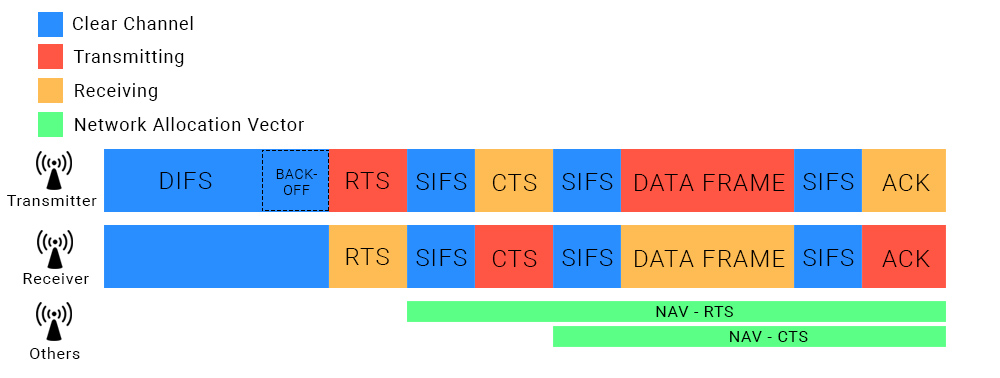
\includegraphics[scale=0.35]{Images/DCF.jpg}
	\caption{The timeline one frame transmission cycle in DCF mode}
	\label{fig:dcfmode}
	\end{figure}



	\section{PHY Layer}
	The physical layer in 802.11 is also divided in two sub-layers. The upper sub-layer is the Physical Layer Convergence Procedure (PLCP), responsible for clear channel assessment and acting
	as a common interface for MAC layer drivers. The lower sub-layer is the Physical Medium Dependent (PMD) which is responsible for modulation and directly interfaces with
	the radio. It is responsible for transmitting the complete frames, as well as receiving and decoding incoming frames. 

	\subsection{PLCP Protocol Data Unit}
	The physical layer convergence procedure creates PLCP Protocol Data Units (PPDUs), 
	that consists of 3 parts. The preamble, the header and the frame from the MAC layer
	called MAC Service Data Unit (MSDU). The frame structure
	has a long and short format, and changes a little bit for High Rate DSSS (HR-DSSS),
	but contains mostly the same fields.

	%\begin{figure}
	%\center
	%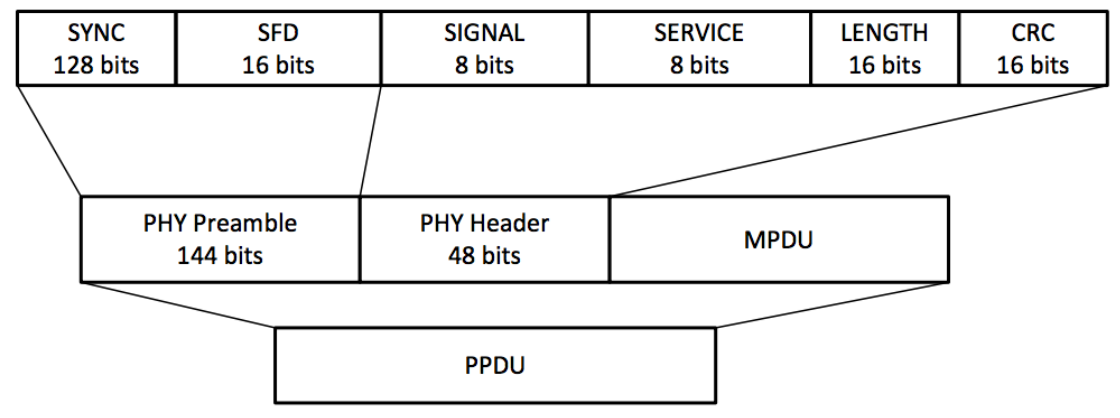
\includegraphics[scale=0.5]{Images/PPDU.png}
	%\caption{DSSS PHY PPDU format from IEEE Std 802.11-2016  }
	%\label{fig:PPDU}
	%\end{figure}


	\begin{itemize}
	\item \textbf{Sync} bits are used to acquire the signal and synchronize timing. 
	\item \textbf{SFD} stands for Start Frame Delimeter and is there to indicate the start of a frame.  
	\item \textbf{Signal} the modulation type used to encode the MPDU and
	the data rate it is sent with. 
	\item \textbf{Service} Reserved for future use. 
	\item \textbf{Length} 16-bit fields that indicates the amount of time (in
			microseconds it will take to transmit the MPDU).
	\item \textbf{CRC} is the cyclic redundancy check that protects
	the fields signal, service and length. 
	\end{itemize}

	\subsection{Clear channel assessment}
	The PLCP layer provides clear channel assessment.
	The purpose of clear channel assessment is to give information to the MAC
	layer if the medium is available for transmission. There
	are primarily two ways the physical layer does CCA.
	\begin{itemize}
	\item CCA-ED (CCA-Energy Detect) detects signals that can not be decoded as a 802.11 frame, but is nonetheless a disturbing signal on the channel. If the CCA-ED value
	exceeds a threshold, for instance 20 dB, then the CCA shall be indicated as
	busy by issuing a \verb|PHY-CCA.indication(BUSY)| to the MAC layer.  
	\item CCA-CS (CCA Carrier/Sense) detects a valid 802.11 frame and can
	properly decode the header fields of a valid PPDU frame.
	The channel gets marked as busy for as long as the length
	field in the PPDU header specifies, even if the obvserved
	signal is weaker than the ED threshold. 
	\end{itemize}

	\section{Radio Frequency Interference}
	Radio Frequency Interference (RF-interference) is the result
	of two or more signals being transmitted on the same frequency at the same time.
	A receiver will have problems deciding which parts of the signals 
	belongs to which transmitter, and the signal may altered to the extent
	that bits are changed or misrepresented. As the 2.4 GHz band that 802.11
	utilizes is a part of the Industrial, Scientific and Medical (ISM) band, channel noise or interference
	can come from sources such as microwaves, bluetooth devices and radio controllers, in addition to other Wi-Fi devices. 

	\subsection{Impact in 802.11}
	If the PPDU header
	gets corrupted by an interfering signal and can not be decoded
	, the PLCP layer issues a \verb|PHY-RXEND.indication(CarrierLost)|
	to the MAC layer. According to CSMA/CA the station then has to
	wait EIFS (Extended Interframe Spacing) time before
	it can transmit a new frame. EIFS is defined as
	\verb|ACK transmission time + SIFS + DIFS.| This is because the station that received the corrupt frame have no idea if any neighbouring station
	received it correctly, and is about to transmit an ACK-frame in response. Additionally
	to waiting the minimum EIFS time, the station also has to wait for
	an idle channel indication from the PLCP layer again. 

	This is just the added delay if a collision happens. Of course, the more co-channel interference, the more transmitters are waiting for medium access, meaning
	the contention window will increase, and the frequency of which a transmitter is granted access to the medium will be reduced. Thus, interference is severely damaging for QoS on wireless networks.   % The correct formula for EIFS is $DIFS + SIFS + lowest transmission time" 

	\subsection{Countermeasures}
	Several countermeasures to limit the impact of RF-interference has been suggested.
	On the MAC layer there is frame aggregation with individual headers.
	Frame aggregation in 802.11n is a technique that wraps several payloads under the same
	header and send them together at the same time, once channel access is granted. This can improve the throughput
	if the channel is clear, but if the frame gets corrupted during transmission
	an increased amount of data is lost.
	Therefore it can be beneficial to aggregate a frame with individual headers.
	Even though this gives a slightly increased processing and transmission overhead
	compared to regular aggregation where there is no individual headers, 
	each frame can be selectively acknowledged.
	This means that only a few frames has to be retransmitted in case of corruption,
	and not the entire aggregation. 

	Additionally on the physical layer there are a couple of other suggested countermeasures:
	\begin{itemize}
	\item Changing the transmission power levels
	\item Lowering data rates
	\item Adjusting CCA threshold
	\item Forward error correction
	\item Changing packet sizes
	\end{itemize}


	\begin{wrapfigure}{R}{0.25\textwidth}
		\caption{\newline Channel distribution}
		\label{fig:channels}
		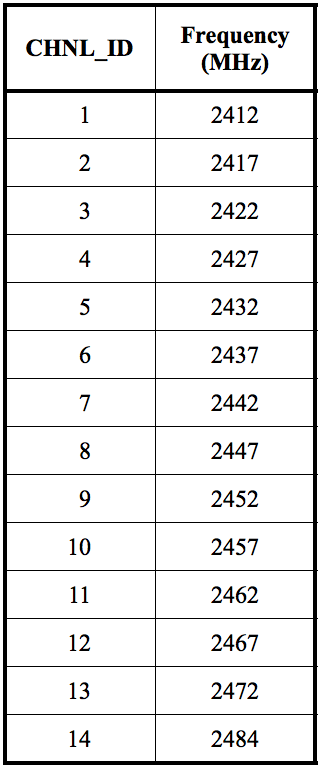
\includegraphics[width=1\linewidth]{Images/Channels80211.png}
	\end{wrapfigure}


	The mentioned countermeasures only have limited
	impact, while switching to a channel with less interference (if available) remains the most effective in most cases \cite{impactRF}. 
	\section{Channels} 
	802.11 b/g/n uses the range of frequencies from 2.400-2.500 GHz on the ISM band.
	The increasingly popular 802.11n/ac also uses a range of 5 GHz frequencies on the Unlicensed
	National Information Infrastructure (UNII) band, which offers more frequencies \cite{5ghz}.
	Other than that the properties and challenges for the different bands are ultimately the same.
	The distribution of the frequencies on the 2.4 GHz band to the different channels is illustrated by figure \ref{fig:channels}. The frequencies listed are the center frequencies of each channel. In practice this means that an AP that transmits on one channel will interfere with close channels in both directions. Two channels are entirely non-interfering if they send on two frequencies  $f_{1}$ and $f_{2}$ so that $|f_{1} - f_{2}| > 0.025$. This means that there are in total three completely non-overlapping channels, 1, 6 and 11. The process of deciding which channel to transmit on is called channel allocation. 



%\chapter{Channel Allocation}

\begin{itemize}
\item Least Congested Search
\item MinMax
\item MinMax II
\item Hminmax/Hsum
\item Pick-Rand and Pick-First Approach
\item Pick-Rand and Pick-First II Approach
\item Channel Hopping Approach
\end{itemize}

\chapter{Related work}
This chapter is dedicated to give a brief account of works related to solving some of the challenges posed so far in this thesis. It is worth noting that some of the 
works mentioned here are actual implementations and live products, but only deployed in corporate environments.

\section{Cisco RRM}
CISCO offers a solution directed at enterprise networks \cite{ciscoRRM}, where implementing and managing a centralized
controller is a more managable task than in residential networks.
Their architecture consists of one or more Wireless Lan Controllers (WLCs).
The WLCs creates a group name and shares it with all APs in the same RF-group. All APs broadcasts their RF-group name, along
with the IP-address of their controller. Any other AP sharing the same RF-group name reports the incoming broadcast message to the controller, and then rebroadcasts the packet.  This way the controller
becomes aware of all APs that are in range of each other, similar to the flooding routing mechanism,
and they can form logical groups based on this information.
If applicable the RF-groups perform leader election to decide which controller becomes the RF Group leader, but there
can also a preconfigured leader. The RF group leader has the responsibility of running the relevant channel allocation
algorithms and ajusting the radio power level of the APs. 

\section{DenseAP}
DenseAP described in \cite{Murty2} aims to restructure the infrastructure of enterprise networks.  The two fundamental
changes they suggest is to deploy APs a lot denser (hence the name), and moving the task of associating clients
with APs to a centralized controller. The reasoning behind the dense deployment of APs is that signals diminishes
quickly in an indoor environment, and ideally a client should always be associated with an AP in the close vicinity. The argument 
they use for moving the association decision away from the client and over to a central controller, is that a client can
only use signal strength as the metric deciding which AP to associate with. This is emphasized as
suboptimal in conferences and meeting room environments, where many clients seek to associate with an AP at the same time.
If all clients pick the same AP it also means all clients will transmit on the same channel,
and RF-interference can reduce the throughput on the medium. 
Their infrastructure consists of DenseAP access points (DAPs) and DenseAP Controllers (DCs). The DAPs sends periodic
reports to the DC, which contains information as RSSI measures, channel interference, and associated clients. Based on this
information the DC decides which DAP each client should associate with, and also which channel each DAP should transmit
on. 

\section{HiveOS}
HiveOs \cite{Aerohive}, developed by Aerohive Networks offers distributed protocols and mechanisms to improve Wireless LANs in enterprise networks. The APs 
in the network are called HiveAPs, and they offer services such as
\begin{itemize}
	\item Band steering: if an device can operate on the 5Ghz band, it will be forced to connect to the 5Ghz network to optimize the utilization of the radio spectrum. 
	\item Load balancing: all HiveAPs have real-time information about how clients performs. If a client tries to associate with a new HiveAP, it will only be accepted
				if the new HiveAP has a low enough load to handle more clients. It would also know if other neighbouring APs are better suited to handle the load of the new client.
				This is achieved by witholding probe responses.

	\item Channel allocation: by using the Aerohive Channel Selection Protocol, HiveAPs tries to select the channel with the lowest co-channel interference. Their channel selection protocol uses 5 measurements, two static and 3 dynamic.
	The first static measurements is the number of nearby APs who are operating on the same channel. The more APs there are the higher the penalty. The penalty per AP diminishes as the number of APs increases, this
		is because the first one(s) are the most critical. The other static cost factor is what power level can be transmitted at the given channel, as this may differ on some 5GHz non-overlapping channels. The dynamic measurements are CRC-error rate, channel utlization,
	and the utilization of overlapping APs. All of these dynamic factors can penalize a channel with 0 to 3.5%. 
\end{itemize}

\section{ResFi}
ResFi \cite{resfi} is the only significant related work that directly aims to enable self-organized management in residential deployments of wireless LAN. Works such as \cite{Murty2}, \cite{ciscoRRM} and \cite{Aerohive} are all directed toward enterprise
networks. As we also aim to mainly concern ourselves with residential networks and their infrastrucure, ResFi is especially interesting to look at. ResFi assumes that all access points have two interfaces, one connected to a wired backone (e.g Internet), and another
802.11 compatible wireless interface. The figures of ResFi includes a Radio Resource Management Unit (RRMU). This is simply the device that interfaces with the antenna, and in most residential homes it will be a router that controls the channel and the power levels of the antenna. In short ResFi enables communication between access points under different basic service sets without imposing a central controller on the access points or being a part of an extended service set. More importantly, ResFi enables all of this without doing any modifications to hardware and drivers (like modifying standards or requiring propriatary equipment). 

\subsection{Operation}
This section contains a short introduction of the way ResFi is initiated and operates.
\begin{enumerate}
	\item An AP that has just booted up beacons a frame on all available channels. This frame contains: a globally routable IP-address, port, and two cryptographic keys. One transient key for group communication, and the public key for the RRMU. 
	\item All APs that can hear the beacon responds with a probe response containing the same information as in 1.
	\item When the scan is complete, the new AP can establish secure point-to-point communicate with all other APs using the wired backbone, the globally routable IP-address and the cryptographic keys
\end{enumerate}

\subsection{Implementation}
This section is dedicated to a brief overview of how ResFi can be implemented and deployed.

Originally ResFi was implemented on Ubuntu 14.04. It adds vendor specific information elements to the MAC-header with the IP, port, and cryptographic data. This can be done Linux user space by using their modified version of hostapd \cite{resfigit}.
As it runs on python, it could in practice be implemented on any Linux system. It uses a south-bound API to communicate with the RRMU, and a north-bound API to enable applications to use ResFi. ResFi itself provides no specific channel allocation mechanism nor a group-creation/AP-clustering algorithm, but the north-bound API could fascilitate applications that provides services like these.

%\section{Distributed Clusteering}
%DCA and DMAC

\section{Channel allocation using DSATUR and SCIFI} 
This section is dedicated to previous work done using the DSATUR heuristic. A little note to this section: it would also fit well in the background section. It accounts for the fundamentally important priniciple that
channel allocation can be treated as a graph coloring problem once a network graph is constructed.  

\subsection{DSATUR}
DSATUR (from degree of saturation) is a heuristic created by Daniel Brélaz \cite{Brelaz} to find solutions to the NP-complete problem of coloring the vertices of a graph so that no adjacent vertices share the same color. 
Channel allocation schemes relying on the DSATUR algorithm has been proposed before. In 2004 a paper was published, called
"Automatic channel allocation for small wireless local area networks using graph colouring algorithm approach" \cite{mahonen}, where the idea is to listen for neighboring AP beacon frames to create a list of all neighbours.
This list would be broadcast to all the neighbours. For multi-hop support, all receiving nodes will rebroadcast the list in a fashion equal to the flooding routing mechanism. This enables routers to create a graph of access points, and the DSATUR algorithm can then be used to compute the channel distribution. 

\subsection{SCIFI}
SCIFI \cite{SCIFI} is a centralized channel allocation protocol for infrastructure Wireless LANs that improves the traditional graph-coloring algorithm DSATUR. While it shows that their central coordinator
in fact improves the throughput compared to Wireless LANs that are not configured by SCIFI, the it is an algorithm for setting a channel in a preconfigured adminstrative domain. It does not deal with how the administrative domains
or router clusters are defined. If the method of creating clusters of collaborating routers proposed in this thesis has merit, SCIFI could plausibly be a supporting technology to compute channel distribution,
where a group acts as the administrative domain required by SCIFI. 



\chapter{Data acquisition and data structure}\label{dataacc}
This chapter is dedicated to the creation of a program that generates and visualizes the layout of Wi-Fi network topologies based on generated data and mined data.
The data will be used in chapter \ref{chap:clustering} where there will be demand for data to feed clustering algorithms. Storing the data,
the data structure type, and finally how it can be visualized in a web application are also matters which will be addressed here. 

\section{Motivation}
There is an undoubtful need for data when developing a distributed clustering algorithm to facilitate group creation.
Surely a testbed would also be beneficial for development, but it would require a large amount of routers. Maybe 100-200 for a low scale test, in a small geographical area,
preferably installed in residential apartment buildings. Not only would the creation of such a testbed require a vast amount of equipment, but there are 
some unsolved logical challenges as well. Like the communication protocol between routers, and maybe distributed consensus or some way to perform synchronization to communicate group memberships.
These problems are addressed in chapter \ref{chap:proto}.

Even if such challenges could be overcome, going directly from a concept idea to a large testbed in a master thesis  - without having any empirical indication of which approaches have merit, may not be a good use of time. Hence, the data is gathered with the motivation of being able to perform realistic calculations and do algorithm developement on a money-, and time budget. Lastly, the motivation behind mining real data, instead of generating everything, is to enhance the quality and believeability of the results produced. 

\section{Requirements and assumptions}
This section will cover the requirements and assumptions for a data generation-, and visualization program. 

\subsubsection{Background}
As presented in the background chapter: SSID, channel frequency, radio power, physical data rate and supported 802.11 standards are just a few of the properties
that makes up a wireless access point. Before deciding how to represent an access point in a network topology dataset, it is useful to
consider the state an access point would be in when group creation is performed.  

An access point is not in the transmission (CSMA/CA) state when performing channel allocation. This is simply due to the toughness of performing channel sensing without
having a channel to sense. So, which sate is it in then? Well, it is hard to say without having a bird's eye view of the protocol and algorithm architecture. A fully developed protocol
for distributed group-creation in residential deployed Wi-Fi is at the time of writing (and to the author's knowledge) non-existient.  Nor will a full-fledged architecture be presented in
this thesis (even though suggestions will be made at the end), so a couple of assumptions has to be made. 

\subsubsection{Assumptions}
The access points are in a state we can call the \textit{group discovery state}, where the goal is to find or create a group to be a part of.
The major motivation for doing group creation in the first place is to be able to cleverly and collaboratively allocate channels within the group, so this state would
have to occur before channel allocation is performed. 

Hence, to simulate group creation and discovery, many of the access point properties does not have to be considered. Actually it is only necessary to store two things:
\begin{itemize}
	\item Each access point's SSID, as a convenient way to provide a unique identification handle \footnote{In the real world this is of course not the case,
but we will enforce it in the computations. Actually it could just as well be called an unique id.}
	\item The list of neighboring access points that can be seen through a Wi-Fi interface scan on each access point, along with the observed signal strength of these APs.
\end{itemize}
Channel frequency, radio power and data rate are properties that impacts data transmission between clients and access points, and does not need to a 
part of this model. 

In all succeeding simulations it is assumed that all nodes are transmitting with equal strength, and that the environment is flat and obstacle free. 

\subsubsection{Requirements}
Unfortunately there is at the time of writing no publicly available data source that contains radio scans of a large amount of access points located in the same area.
This subsection describes the requirements for the simulation program that will both generate and represent Wi-Fi network topologies. Having a clear specificiation of program requirements
simplifies the programming stage and reduces the risk of feature creep. 

As a basis for the simulation, access points, hereupon also referred to as nodes, should be placed on a two-dimensional grid. Each dataset has to contain a set of nodes which has two coordinates $x$ and $y$, giving them a position on the grid. When all desired nodes are placed on a grid, the grid represents a network topology. It will then be possible to compute an
estimation of which nodes can hear each other over the Wi-Fi radio. In other words, a virtual network interface scan. All observed \textit{neighbour nodes} will be added to each node's
neighbour list. This neighbour list contains the names of all the nodes it can hear, and the signal strength levels measured in $-dBi$.

Additionally the following parameters should be variable in the topology generation program, depending on each test scenario:

\begin{itemize}
	\item Topology size with the possibility to give variable width of x- and y-axis as input arguments. These unit of the axes is meters. 
	\item Number of nodes to place on the topology
	\item Minimum distance between nodes (in meters). This is only to avoid unlikely placement and extreme interference of nodes that are placed on top of each other. 
	\item Minimum loudness measured in $-dBi$ for a node to account another node as a neighbour (e.g -100 is too low for anyone to hear).
\end{itemize}


	\section{Program design}\label{prog_design}
	\subsection{Primary functionality}
	The resulting program consists of two main functionalitites.

	The first functionality is creating a topology and generate nodes which are uniformly
	and randomly positioned on the network topology. The topology size, node count and minimum distance
	between nodes, are properties taken as input arguments to the program.

	The second functionality is performing the calculation of which nodes can actually observe each other over the radio, and is described below.

	\subsubsection{Signal strength calculation}
	\begin{figure}
		\begin{python}
			#In topology class
			def measureInterference(self):
			for nodeSubject in self._nodes:  
			for nodeObject in self._nodes:
			nodeSubject.calculateInterferenceTo(nodeObject) 

			#In node class
			def calculateInterferenceTo(self, nodeObject):
			if self == nodeObject:
			return
			dist = round(self.distanceTo(nodeObject))

			#If  nodes have same coordinate, set high interference. 
			if (dist == 0):
			dBi = -40
			else:
			dBi  = self.measureDbi(dist) * -1

			def measureDbi(self, dist):
			return (20 * math.log(self._frequency, 10)) + 
			(20 * math.log(dist, 10)) - 27.55

		\end{python}
		\caption{Computing the interference between nodes}
		\label{fig:dbiCreation}
	\end{figure}

	All neighbouring nodes observed by a node is added to its list of neighbours. The neighbour list contains the signal strength in $-dBi$ and the SSID of each neighbour.
	The interference levels between access points are calculated by iterating through every access point. For each node $N$ its x and y position is recorded,
	and then a second iteration through the nodes is initiated, resulting in a complexity of $O(N^2)$. For each node $n$ in the second iteration the distance $d$ in
	meters between $N$ and $n$ using Euclidean distance is calculated.
	
	To compute the signal strengths of which the nodes can observe each other, the formula for isotropic antennas, described by Friis \cite{Friis46}, can be used to
	derive the formula for the Free Space Path Loss (FSPL) in dB. 
\[
	FSPL(dB) = 10\log_{10} \left( \frac{ (4 \pi f d)}{c} ^2 \right) 
\]	
	Where $d = distance$, $f = frequency$ and $c=constant$. The constant $c$ is used to account for different units. Meters is used to denominate distance in the program,
	and megahertz for the frequency. The resulting formula implemented in the program is then: 
\[
	FSPL(dB) = 20\log_{10}\left( f \right)  + 20\log_{10} \left(d\right) - 27.55
\]	
	Pseudocode for the interference calculation can be seen in figure \ref{fig:dbiCreation}. 

	\subsubsection{Program result}
	The resulting program, written in Python 3 \cite{Python3}, contains an importable \textit{topology class}. This way, for further testing different data
	sources can be used to get the positions of nodes, and only let the topology class compute the list of neighbours and standarize the data structure of a topology.

The program can be run in the following way
\begin{verbatim}./GenerateTopology.py -n 500 -w 100 -h 100 --space 10 --dbi 80 \end{verbatim}
Which instructs the program to create a topology with 500 nodes. The topology should be 100 by 100 meters large, and there should be at least 10 meters
between each node. The $dbi$ parameter makes sure that only nodes which can be heard with a $-dBi$-value of $-80$ or larger should appear in the neighbour list. 

The entire program can be viewed on GitHub: \newline
{\small \url{https://github.com/hansjny/GroupSimulations/blob/master/GenerateTopology.py}}


\subsection{Data output and visual representation} \label{simulationrep}
The result of the topology generation is stored in a JSON \cite{JSON} data file.
The data file contains the height and width of the the generated topology, as well
as the number of nodes.
A \verb|node| object consists of as many JSON node-objects as there are nodes. Figure \ref{fig:nodeStruct} illustrates the node structure and is an example of how a node with two neighbours will look.
			\begin{figure}
			\begin{minipage}{\linewidth}
			\begin{lstlisting}[language=json]
{
  "mapWidth": 100,
  "mapHeight": 100,
  "nodeCount": 3,
  "nodes": {
    1: {
    "posX": 50,
    "posY": 50, 
    "ssid": "NODE1", 
    "neighbourCount": 2, 
    "neighbours": {
      0: {
        "ssid": NODE2,
        "dbi": -77.23
        },
      1: {
        "ssid": NODE3,
        "dbi": -79.52
        }
      }
    }
  },
...
}
\end{lstlisting}
\end{minipage}
\caption{JSON output structure}
\label{fig:nodeStruct}

\end{figure}

The output from the program execution described in the previous subsection is a 23.2 MB large file containing the resulting topology-data in JSON.

By writing a simple HTML and JavaScript browser application, the JSON can easily be parsed and visually represent the nodes on a grid.
The result after creating a topology and visualizing in the web application can be seen in figure \ref{fig:randtop}.

\begin{figure}
\center
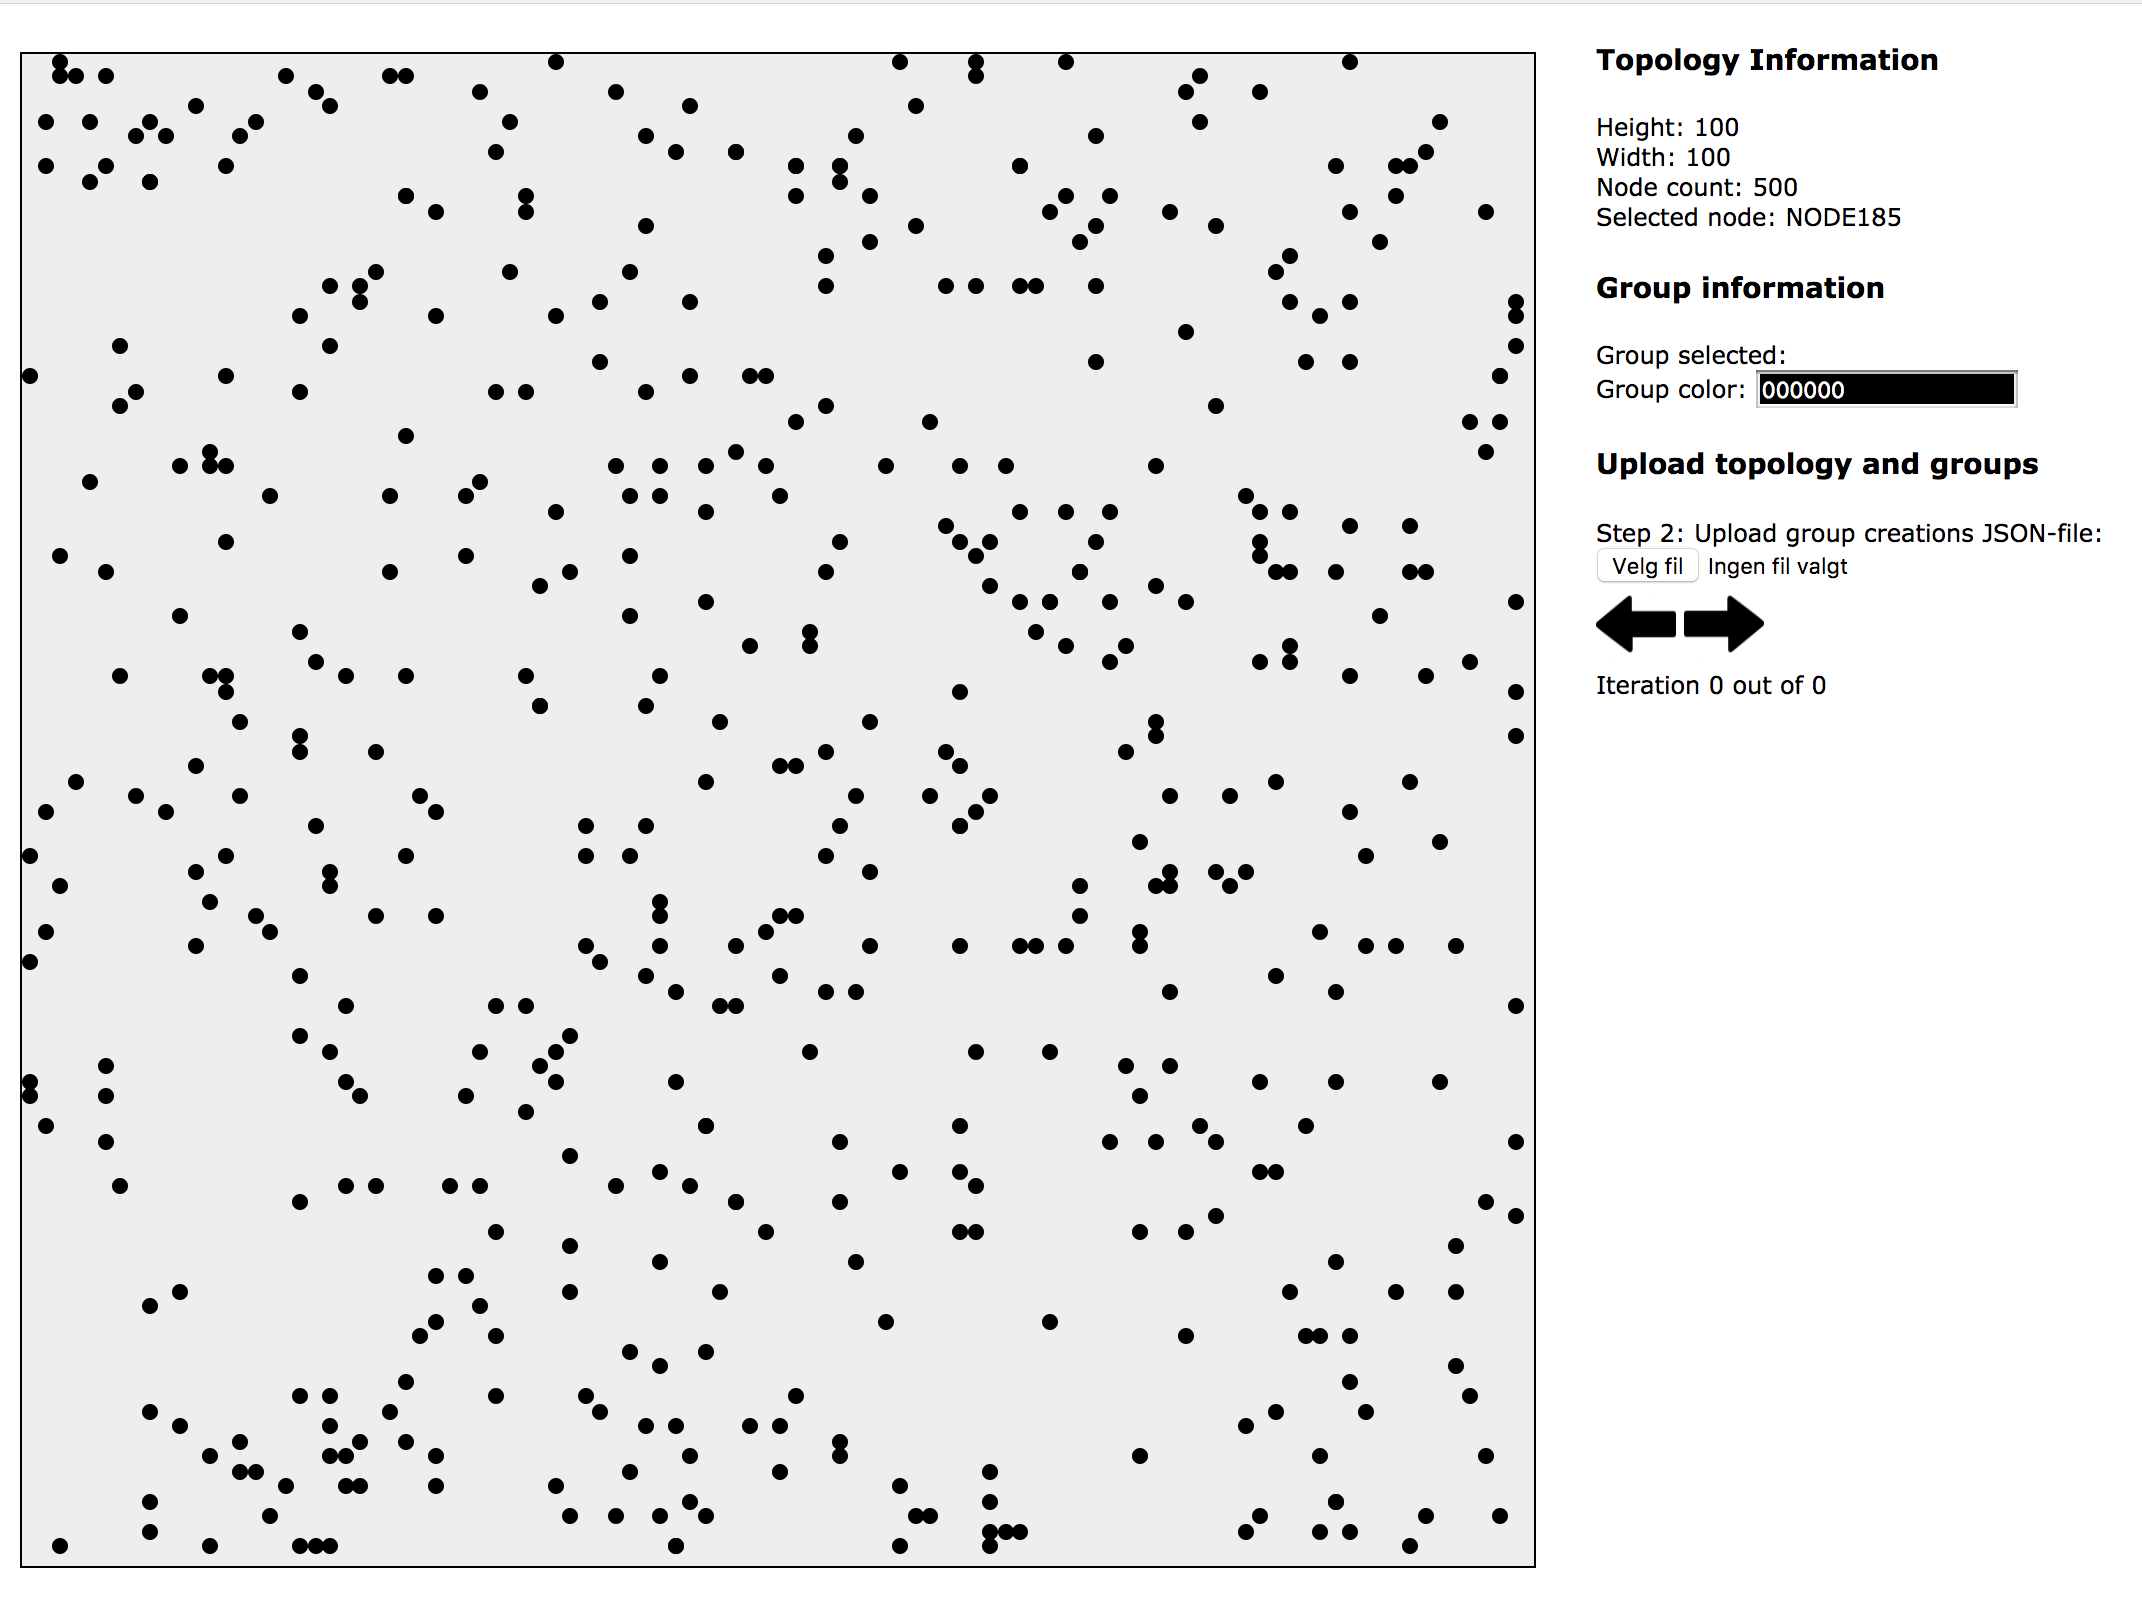
\includegraphics[scale=0.3]{Images/interface.png}
\caption{Generated topology with random, uniform distribution and the interface for viewing topologies}
\label{fig:randtop}
\end{figure}

\section{WiGLE as a data source}
In the previous section we looked at the data generation, representation and visualization of nodes in a network topology with uniform distribution. This section is dedicated
to using an open data source called WiGLE to create the network topology, while reusing the code and data structure for representation and visualization. 

\subsection{Introduction to WiGLE}
The Wireless Geographical Logging Engine (WiGLE) \cite{wigle} is a project started in 2001 which purpose is to gather information about wireless networks.
All information collected by WiGLE is user submitted. Anyone can download an Android app developed and published by WiGLE, and use the app for wardriving\footnote{Wardriving is the act of tracking wireless networks using a laptop or a phone, and then store the network meta data.},
then submit the data to WiGLE's centralized database. The APs discovered can be viewed on an interactive map provided on WiGLE's website as seen in figure \ref{fig:wigfig}.
All the data can also be accessed through a public API. Using their service is entirely free, but the amount of data that can be requested is throttled on a day-to-day basis.
In the FAQ section on the website its written that the project openly supports research projects, so after contacting them they upgraded the account which will be used to gather data
for this thesis to a higher daily data limit. 

\begin{figure}[h]
	\center
	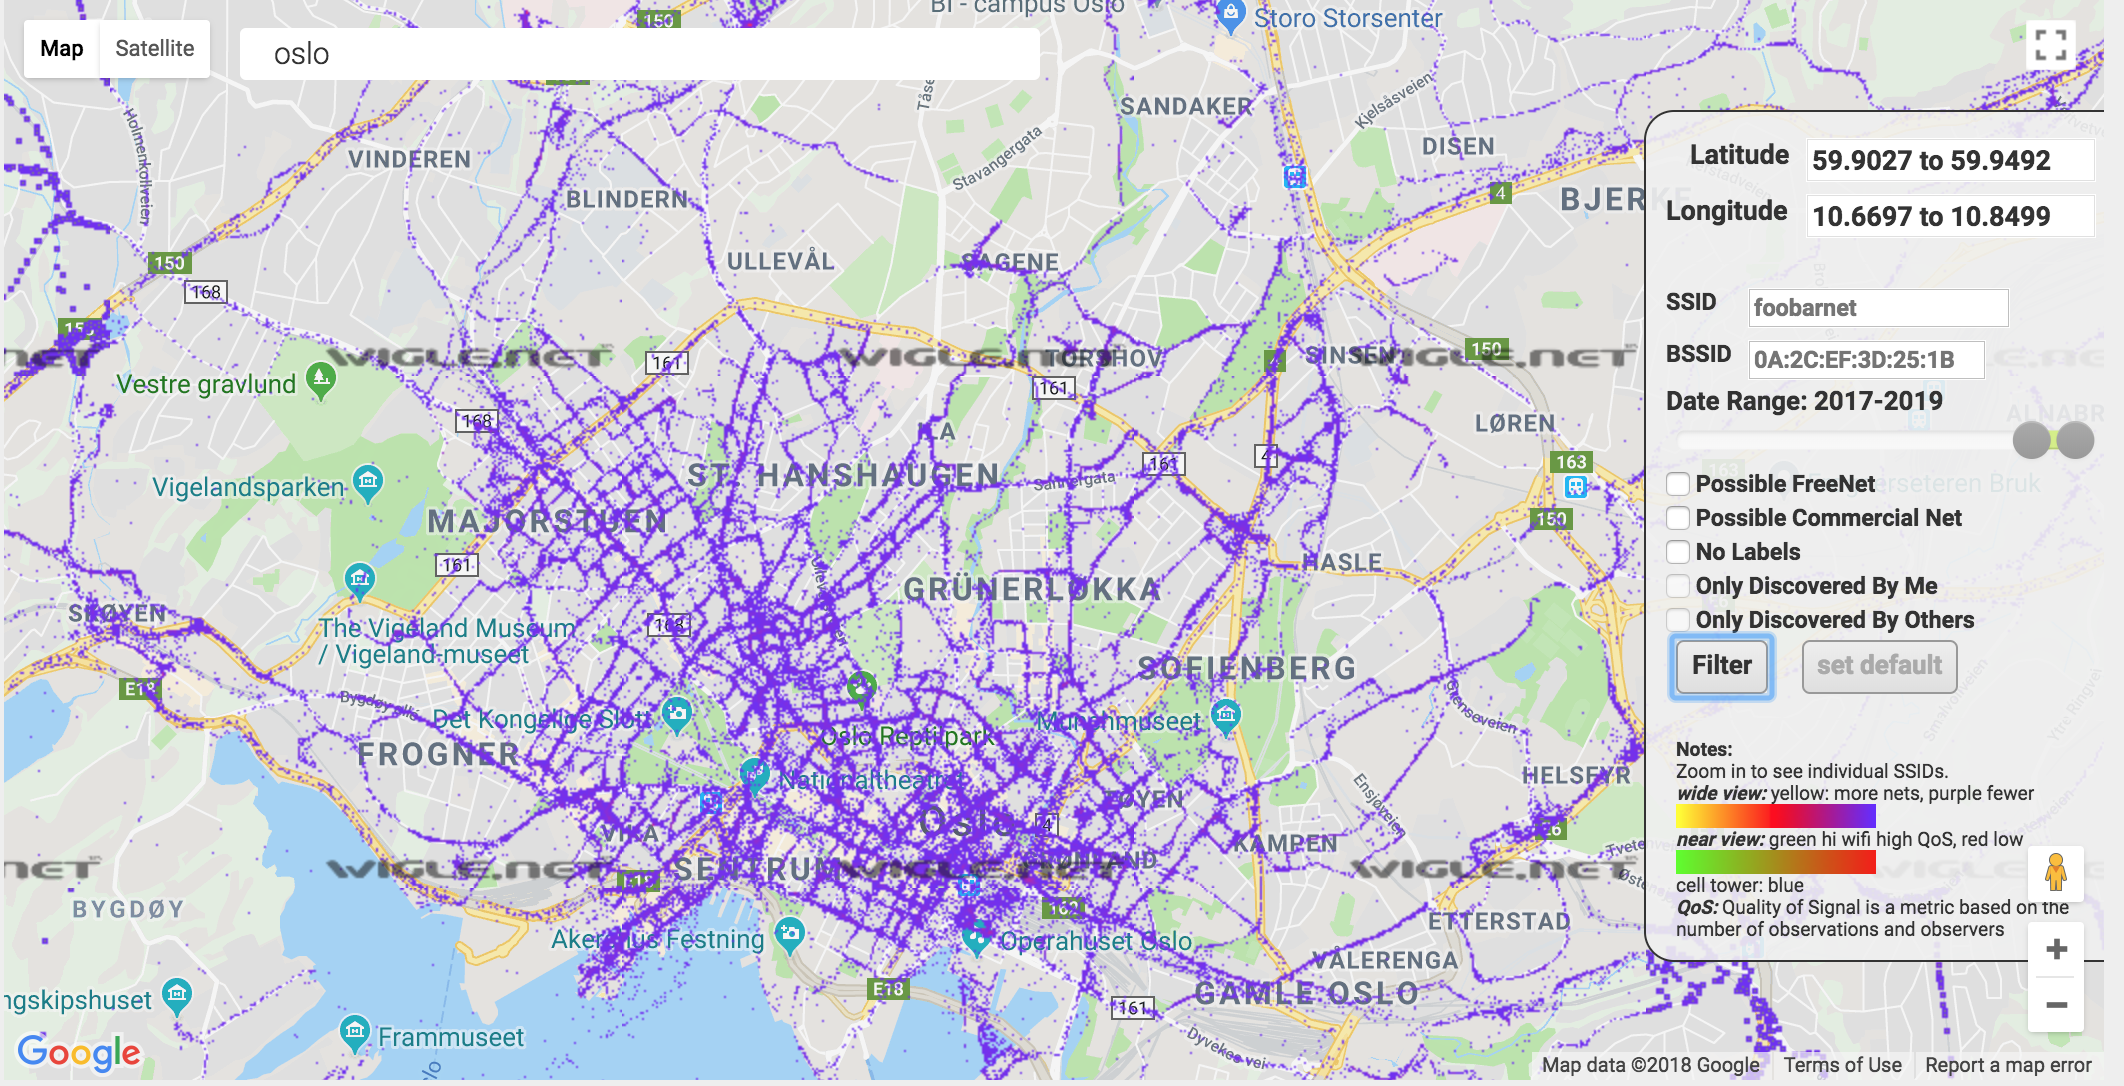
\includegraphics[scale=0.35]{Images/wigle.png}
	\caption{WiGLE map of Wi-Fi networks observed in Oslo from 2017-2018}
	\label{fig:wigfig}
\end{figure}

\subsection{Data quality}
WiGLE determines the geographical coordinates of the position of each access point using weighted-centroid trilateration \cite{Sharma}. 
This means the AP location is not necessarily accurate:
if the measurements of an access point signal strength is done in multiple places (in a way that a line between the measurement locations surrounds the access point),
the access point location becomes very precise. On the other hand, if the measurements are taken on only one side of the access point,
the measurements are heavily shifted towards that side. This tendency can be observed
when zooming in on many Norwegian towns where most access points seem to be positioned on the road. This is obviously not right, but as most observations
are most likely are done from the road when wardriving, this happens frequently. Figure \ref{fig:wiglediff} illustrates the big difference multiple observation points can make.

Even though the data is not perfect, it is safe to say it is better suited to impersonate the layout of real-life network topologies than the generated data.

\begin{figure}
	\centering
		\subfloat[Few observation points in Ski, Norway]{{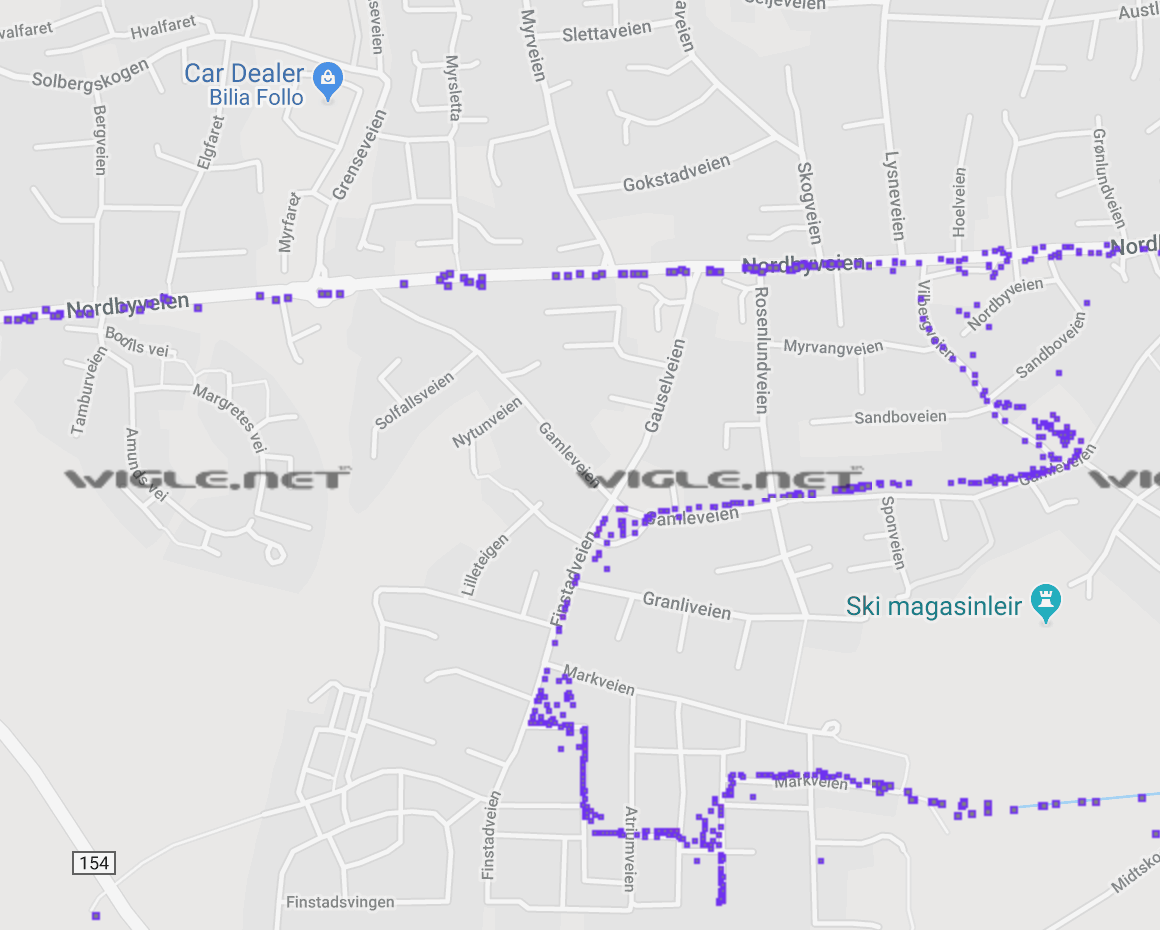
\includegraphics[width=6cm]{Images/wigleSki.png} }}%
		\qquad
		\subfloat[Several observations points in Manhattan, New York]{{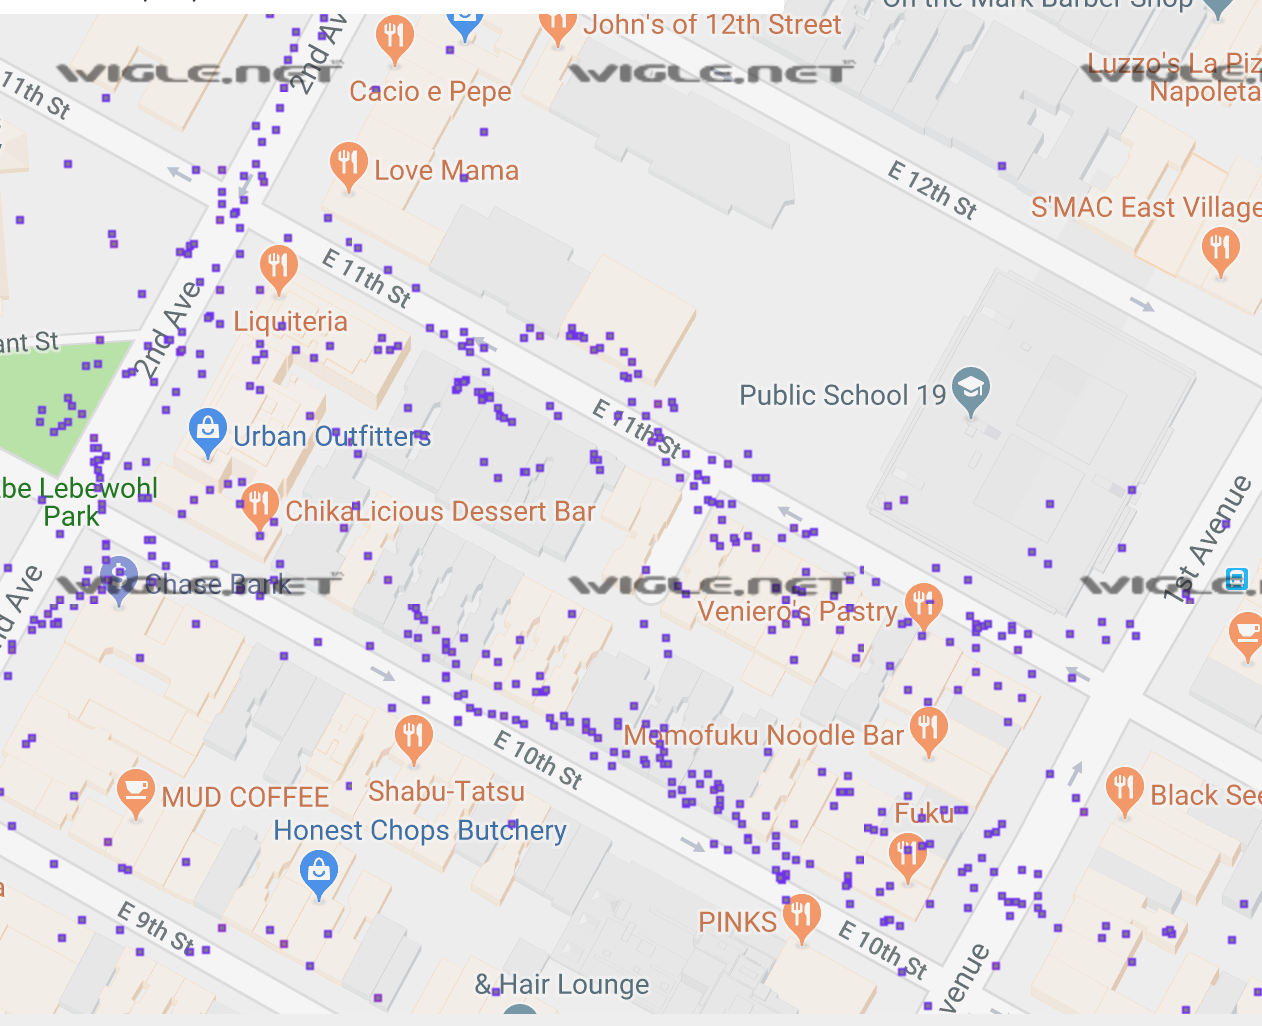
\includegraphics[width=6cm]{Images/wigleNy.png} }}%
		\caption{WiGLE accuracy}%
		\label{fig:wiglediff}%
\end{figure}

	\subsection{REST API}
	\subsubsection{Overview}
	WiGLE has a REST API that can be used to retrieve information from their database. The API responds to requests with JSON data. It gives access to a
	number of services such as user profile management, large-scale statistical information about the collected data
	and more specific network searches. An interactive guide to the public API is available at \cite{WigleAPI}. 

\begin{figure}
	\scriptsize
	\begin{lstlisting}[breaklines]
	 https://api.wigle.net/api/v2/network/search?first=0&latrange1=37.80846&latrange2=37.7467&longrange1=-122.5392&longrange2=-122.3813&start=0
	\end{lstlisting}
	\caption{Example of a Wigle API request}
	\label{fig:wigReq}
\end{figure}


	\subsubsection{Data gathering}
	To retrieve data for the topology generation progam, the only required part of the API is the network search service. There are several ways an access point can be retrieved using
	the network search. For instance specific SSIDs can be queried, a range of coordinates, APs with a minimum signal level, or only query networks that are free to use. As 
	the purpose is to rebuild the network topology to fit the previously tailored data structure, all access points will be considered, and no filters applied except for a range of coordinates.
	By issuing an API request for nodes between two latitudes and two longitudes, the response is an array with AP objects within that area.  
	An API request will look something like what can be seen in figure \ref{fig:wigReq}. 
	The parameters $latrange1$ and $longrange1$ are the coordinates that marks the beginning of the area of interest, while $latrange2$ and $longrange2$ marks the end. 
	To be meaningfully create a network topology based on the API request, information about \textit{all} access points within the specified range is desired. Alas, as it happens
	WiGLE returns at most 100 results per query. This means if there are more than 100 access points, the $start$
	parameter has to be changed. This parameter tells WiGLE at which offset to begin fetching data from. For instance a start value of $0$ instructs it to fetch the first 100 access points, with indexes 0-99. A value of $100$ means that the next 100 APs in the range $100-199$ is fetched, and so on. The JSON response for a succesful request for one AP can be seen in figure \ref{fig:wigle}. 

	\begin{figure}

	\begin{lstlisting}[language=json]
{
	"userfound": false,
	"qos": 0,
	"comment": null,
	"lastupdt": "2015-12-22T17:49:34.000Z",
	"bcninterval": 0,
	"dhcp": "?",
	"lasttime": "2015-12-22T17:49:15.000Z",
	"trilong": 10.82792618,
	"netid": "5C:9E:FF:2B:54:84",
	"freenet": "?",
	"trilat": 62.2816925,
	"name": null,
	"firsttime": "2015-12-22T20:55:01.000Z",
	"type": "infra",
	"ssid": "NETGEAR23",
	"paynet": "?",
	"wep": "2",
	"transid": "20151222-00207",
	"channel": 52
}

\end{lstlisting}
\caption{REST API response with AP data}
\label{fig:wigle}
\end{figure}

The JSON-object in the response contains quite a lot of information about all of the APs retrieved. Most of this data is redundant information, but it is worth noting that some of it could be used to perfect the search. For instance the "last updated"-parameter could be a way to refine the access points retrieval so access points which have been long gone is not fetched. The most valueable properties are $trilong$ and $trilat$. As the names suggest these contain the estimated coordinates of the access points. 

\subsubsection{The Haversine Formula}
As seen in the previous section, WiGLE provides data about the location of access points and a way to retrieve this data in a usable format. 
At this point a program that operates directly on the retrieved longitudes and latitudes could be made, but the problem is that the previous work relies on a two
dimensional Cartesian coordinate system. To be able to reuse what we have have already built, the global coordinates has to be translated into distances.

The haversine formula \cite{virtues} can be used to accurately compute the great-circle distance between two global coordinates.

\[
	d =2R sin^{-1} \left(\sqrt{ \left(sin\left(\frac{\varphi_2-\varphi_1}{2} \right)\right)^2 + cos(\varphi_1) * cos(\varphi_2) * sin\left(\left( \frac{\lambda_2 - \lambda_1}{2} \right)\right)^2} \right)
	%a = sin²(Δφ/2) + cos φ1 ⋅ cos φ2 ⋅ sin²(Δλ/2)
	%FSPL(dB) = 20\log_{10}\left( f \right)  + 20\log_{10} \left(d\right) - 27.55
\]	

Where $d$ is the distance between two latitudes $\varphi_1$ and $\varphi_2$ and two longitudes $\lambda_1$ and $\lambda_2$. $R$ is the radius of the
sphere, which in this context is the earth's radius. 

This can also be expressed with a two-parameter inverse tangent function \cite{chamberlain_2017}, as long as neither of the
parameters are zero. 

\begin{flalign}
	\nonumber a &= \left(sin\left(\frac{\varphi_2-\varphi_1}{2} \right)\right)^2 + cos(\varphi_1) * cos(\varphi_2) * sin\left(\left( \frac{\lambda_2 - \lambda_1}{2} \right)\right)^2 \\
	\nonumber c &= 2*atan2(\sqrt{a}, \sqrt{(1-a)}) \\
	\nonumber d &= c * R
	%a = sin²(Δφ/2) + cos φ1 ⋅ cos φ2 ⋅ sin²(Δλ/2
	%FSPL(dB) = 20\log_{10}\left( f \right)  + 20\log_{10} \left(d\right) - 27.55
\end{flalign}


The python implementation of the formula can be seen in figure \ref{fig:haversine}. It is imortant to note that the degrees taken as input
has to been converted to radians before inserting it in the formula. 

	\begin{figure}[H]
		\tiny
		\begin{python}
def distanceBetweenCoordinates(lat1, lat2, long1, long2):
	deltaLon = math.radians(long2 - long1)
	deltaLat = math.radians(lat2 - lat1)
	a = (math.sin(deltaLat / 2))**2 + math.cos(math.radians(lat1)) * math.cos(math.radians(lat2)) * (math.sin(deltaLon/2))**2
	c = 2 * math.atan2(math.sqrt(a), math.sqrt(1 - a)) 
	R = 6371000
	d = round(c * R)
	return d
	\end{python}
			\caption{Implementation of haversine distance}
			\label{fig:haversine}
	\end{figure}


This function is used to compute the distance in meters between the boundaries of the area of interest. When data is retrieved from
WiGLE, the specified coordinate range is used to compute the size of the cartesian coordinate system, and it is done in the following way:
\begin{itemize}
	\item Compute the distance between the first latitude $\varphi_{start}$ and the second latitude $\varphi_{stop}$ and returns the size of the x-axis in meters.
	\item The opposite has to be done to get the size of the y-axis, using the distance between $\lambda_{start}$ and $\lambda_{stop}$. 
	\item The same approach is used to place each node on the coordinate system, where the first set of the coordinates is
$\varphi_{start}$ and $\lambda_{start}$, and the second set is the coordinates of the AP.

\end{itemize}
\subsection{Data output}
The resulting python program\footnote{GitHub URL: https://github.com/hansjny/GroupSimulations/blob/master/wigleData.py} takes an output filename and two latitudes and two longitudes as input.
It queries WiGLE's API for all the APs between these coordinates. As long as the number of APs in the coordinate range does not exceed the daily data limit, all the data will be stored in a topology datastructure imported 
from the topology generation program in section \ref{prog_design}. The APs will be placed correctly relative to each other, with real world distance between them,
based on the coordinates of each AP. 



\chapter{Access point clustering} \label{chap:clustering}
%To enable collaborative channel allocation, it is
%important for every AP to know which APs it is collaborating with.
%One way to share information about who collaborates with who,
%is to let the access points group together. Information relevant for channel
%allocation can then be shared freely within the group, between APs.

%We will proceed by looking at some of the requirements for a group creation algorithm.
%It should work decentralized in a distributed fashion. Hence, not only does the APs have to
%be imposed group membership, but they also have to be able to create and definine
%meaningful groups on their own. Later we will propose an algorithm to create groups,
%and then evaluate computed groups based on the algorithm.


\section{Introduction}
While it at first sounds incredibly desirable to let the entire population of for instance New York's access points organize themselves in an optimal channel-plan,
at second thought the idea may prove to be a little ambitious. If an optimal channel distribution is to be computed within the group using e.g. DSATUR \cite{Brelaz} which
is an NP-hard problem, we have to set some reasonable constraints on the size of the collaborating group. The amount of nodes that will collaborate on the problem of finding an optimal channel distribution plan may not need to be very high.

Let us for a moment look at an ideal example: a city that only consists of small apartment buildings that are entirely isolated from signals from other adjacent apartment buildings.
How could we build a group in such a case? Turns out it is not that hard. Each access point would be able to collaborate with every other observable access point. A simple flooding mechanism
as suggested by a paper from 2004\cite{mahonen} and described in section \ref{chap:dsatur}, could allow routers to discover each other. When computing channel distribution there would be no risk of surpassing the viable amount of nodes to compute the distribution for, as the groups would naturally be limited to the apartment building.

Alas, in the real world this would not be not be possible. The density of Wi-Fi deployment today is too high, and it is not impossible that every access point in e.g. Manhattan can observe each other through a transitive relation. This means that if a method that simply floods the network to create a collaborative groups was to be used, the amount of nodes in the group could end up being millions.
Flooding mechanisms would saturate the network with update mechanisms, local list describing which other nodes was in the group would be too large. Coordination between millions of peers
is not only infeasible, but also redundant. There is no need for a node on the north side of Manhattan to cooperate with one located in the south. 

This does not mean that creating reasonably sized groups of access points is impossible, but it poses a more difficult challenge. 
We need to filter out less impactful nodes to create an approximated version of the ideal example.

Having a picture of a typical cityscape in mind, we know that buildings are naturally separated by streets, bridges, parks, and so on. Rural areas are similar, but networks are spaced more unevenly and usually only affecting each other in one plane. Hence, the geographic distribution of access points is far from uniform. The problem addressed in this chapter is finding a method for access points deployed in a chaotic and unplanned landscape to group together in clusters of access points. This can either be solved with a centralized coordinator or with a peer-to-peer distributed protocol with a distributed clustering algorithm. In this thesis we will be focusing on the distributed clustering algorithm. 

%\subsection{Centralized model}
%%Just like a distributed version, a centralized controller is also restricted by the NP-hard nature of all graph colouring algorithms if that is to be used to select channels. 
%To be able to compute a channel plan using heuristics, it also has to identify groups of nodes that impacts each other severely. 
%
%The advantage of the centralized model is the ability to have the full picture of access points readily available. Let us assume the controller is placed at an ISP, which might be plausible 
%for residential deployment.
%The controller could potentially know exactly where in the world the access points are placed, by either location reporting or as a part of the information required
%to set up a subscription. Creating groups could potentially be done by dividing access points into groups defined by sections of a map, 
%where the sections are found by observing naturally separative geographical barriers like roads, streets and buildings. This would be like predefining RF-neighbourhoods, 
%if we are to use Cisco's terminology from \cite{ciscoRRM}. 
%
%For a central controller to be able to identify APs that are near each other and compute the optimal channel distribution, APs need to report their radio readings to the controller. 
%The controller then needs to identify which of all the observed APs it can control, and which is not controllable and has to be treated as noise. There would be no requirement for
%communication in between nodes, which reduces complexity a lot.  
%
%A major drawback of the centralized approach is that nodes that are near each other have to be under the same controller. If there are too many nodes around
%that can not be controlled by the controller, all nearby access points would be treated as noise and regular channel allocation schemes would have to be applied.
%Even though in there is a tendency for apartments in the same building to have the same Internet Service Provider in Norway, there is no guarantee for that to always be the case.  
%%Also such controllers does not scale very well and they are single points of failures. 

\section{Distributed group creation}
In the related work section, we presented a couple of centralized solutions. As we want to propose a solution that works across private consumer networks as well as larger corporate networks,
we can not assume that all networks are under the same administrative domain. This is where the centralized approach is limited, and why most solutions presented in the related work section is usually only deployed under the same extended service set, or at least confined to the boundaries of an enterprise. Here we will discuss the benefits and challenges of a distributed model  

\subsection{Benefits}
A distributed approach has the advantage of being scalable and requires less administration and maintenance like central controllers would. 
While the distributed approach also requires other nodes in the network to run the same technology stack to be useful, this could potentially be easier to achieve.
If the technology does not require proprietary software and hardware and is open source, it would be easier for vendors or ISPs to include the technology in their products.
It would benefit all customers, without imposing any significant scalability or administration costs for the providers. Another option for a distributed solution is going through
802.11 standardization. This would make sure all 802.11 compliant access points would be a part of the clusters. 

\subsection{Challenges}
Of course the distributed approach has some major challenges that has to overcome. Here are the most prominent ones: 
\begin{enumerate}
	\item \textbf{The group creation algorithm.} Based on the signal strength and the communication channel, nodes have to be able to organize themselves in a tight cluster of nodes that
		includes all nodes that impacts each other most severely. This problem is the distributed clustering problem that will be addressed in the rest of this chapter.
	\item \textbf{The communication channel}. In a finished implementation of the group creation algorithm from step 1, access points would need to be able to communicate with each other.
		The 802.11 standard does not specify any protocol for communication between access points that are not on the same extended service set.
		This communication would have to happen on the network layer, preferably over TCP for reliable delivery of protocol message, and the communication channel would have to convey messages that enables group creation, most likely a custom application layer protocol. 
	\item \textbf{State synchronization}. As all nodes should be able to compute a channel plan for the group they need to have synchronized information about the members of the groups
		and every members' signal strength measurements. Else the results of the channel distribution would be different for different nodes, and provide little real world value. 
	\item \textbf{Channel distribution calculation}. Even though the centralized approach would have a similar problem, it will be more difficult to solve in a distributed fashion as 
		it is reasonable to assume that an access point has less computational power than a centralized controller.
\end{enumerate}


\section{Clustering assumptions and requirements}
We will be using the data created in chapter \ref{dataacc} to simulate group creation in network topologies. The data provides a topology of nodes where all nodes have a list of neighbouring nodes.
Just as real life access points can scan for neighbouring networks, this neighbour list contains the appropriate computed signal strength measurements for each node.

\subsection{Clustering requirements}\label{chap:requirements}
\begin{enumerate}
	\item Clusters must be formed based only on the locally available information at each node. This means that nodes have no concept of their position, 
		nor their relative position to their neighbours. All information available to each node is the SSIDs of its neighbours as well as the signal strength of these neighbours. 
	\item The clustering algorithm has to be dynamic. Meaning that when nodes appear or disappear it can adjust for the changes in the network topology.
	\item The clustering algorithm needs to be able to adjust its size to a given maximum size. We do not make any suggestions for what this maximum size should be, but
		we have used 128 as the maximum size for the rest of the thesis. 
		\item When clusters are being formed, the border between two different groups should be placed in such a way that the signal strength between the two access points that disturbs each other the most, is as minimal as possible. This is to ensure that the access points that would interfere the most heavily with each other ends up in the same group.
		\item Has to work without a proper bi-directional signal strength between nodes. Meaning that a node can observe another node stronger or weaker than the strength itself is observed at. 
\end{enumerate}

\subsection{Assumptions}\label{chap:assumptions}	
		To simplify the computation procedure and to reduce the workload for building the simulation program we are going to make a number of assumptions:
    \begin{enumerate}
    \item Assumption 1: All nodes involved in the simulation also run the group creation algorithm. There exists no "rogue"-nodes.  
		\item Assumption 2: When a node is observed over radio, it is also known how to directly contact the node (e.g. via TCP). This assumption implies that there exists a protocol that lets nodes communicate and exchange information about their signal strength measurements and group membership. For now we will assume this is true, but in chapter \ref{chap:proto} this issue will be discussed. 
		\item Assumption 3: All the nodes in a group are completely synchronous, and always have an equal image of the state of the group at a given time. This means that through the communication protocol, all nodes in a group are aware of all members' neighbours and their respective signal strengths. Sharing of this information with the group is instant. This is also an issue that will be addressed in chapter \ref{chap:proto}. 
    \end{enumerate}
\section{Program design}
\subsection{Design choices}
The simulation program is designed to be modified so it can accommodate different algorithm variations without changing the fundamental framework.
Everything regarding group computation is implemented in Python 3 \cite{Python3}, and is designed to parse the output from the data generation program from chapter 4, and use it directly.
The data generation (or fetching) is a slow process and should only be done once every time a new data set is required.
The decision was made to not parallelize the program to keep results consistent and to more easily debug and locate program and algorithm implementation mistakes. 

\subsection{Group framework}
The group framework consists of 3 classes with different responsibilities:
\begin{itemize}
	\item \textbf{Group}. An object of this class is an abstraction of all the nodes that belong to the same group. Because we assumed that all nodes have equal
	information about group membership and signal strength measurements, we can store all the members of each group in a list and let the group object act as a unified entity on
	behalf of the entire group. All the interfaces and logic for forming groups are placed within this class. A method named \verb|iteration|
	has the responsibility of triggering the appropriate action based on the state of the group. For instance adding nodes, removing nodes or merging the group
	with another. This is the part of the code that has to be changed when implementing and changing algorithms. If an action was performed the method returns 1, else it returns 0. 

	\item \textbf{GroupCollection}. An object of this class contains all the groups used in a simulation. Its main functional responsibility is looping through all the groups
	and calling the \verb|iteration| method of each group once. This is done in the GroupCollection's \verb|iterate| method. It accumulates the amount of changes done in all the groups,
	by adding the return values of the Group object's \verb|iteration| method. It also handles the destruction of groups, and bootstrapping of newly created groups.

	\item \textbf{Simulation}. An object of this class handles the bootstrapping of groups, where all nodes (given in the input file) are parsed and
	put in their own grown group. Consequently, at the beginning of each computation the amount of groups is equal to the amount of nodes.
	The Simulation class is also responsible for starting and stopping the simulation itself. After bootstrapping all the groups, the Simulation enters a loop
	where it calls the \verb|iterate| method in the GroupCollections object once every run. All the groups have converged and reached a steady state 
	once the amount of changes returned by the GroupCollection's \verb|iterate| method is equal to zero. The results are written to file.
\end{itemize}

\subsection{Output file structure}
The results of the group computations are written to file. The results do not only contain the resulting division of groups, but to be able to recreate the simulation
visually, the results contains the topology of all nodes and their group membership for each iteration in the simulation process. 
The data is stored as JSON, and the structure can been seen in figure \ref{fig:jsongroup}.
Having the data stored as JSON means that the data is to a large extent language independent.
This allows us to either implement a parser in python for the data and use \verb|matplotlib| to visualize it,
or we can use another application to visualize the data. Since we already have the topology visualizer
written in HTML and JavaScript from chapter \ref{dataacc}, we can extend this program to let us upload a group creation output file. 
		\begin{figure}

\begin{minipage}{\linewidth}
\begin{lstlisting}[language=json]
  "iterations": {
    "0": {
      "0": {
	"groupName": "GROUP0",
        "members": {
          "0": "NODE0"
	},
	"memberCount": 1
    },
      "1": {
	"groupName": "GROUP1",
	"members": {
	  "0": "NODE1"
	},
	"memberCount": 1
      }
  },
    "1": {
      "0": {
	  "groupName": "GROUP1",
	  "members": {
	    "0": "NODE0",
	    "1": "NODE1"
	},
	"memberCount": 2
     }
  }
}
\end{lstlisting}
\end{minipage}

\caption{Group simulation file structure}
\medskip
\small
This particular simulation had two iterations. In the first iteration there were two groups, each with one member node. In the second iteration the two groups has merged to one group, now
containing both nodes. 
\label{fig:jsongroup}
\end{figure}



%\section{Algorithms}\label{algorithm}
%We will consider three possible approaches to cluster access points. First we will look at a minimal and basic approach without any complicated heuristics or algorithms. 
%Next we will consider a well known clustering algorithm and treat the problem as a pure clustering problem. Finally we will look at the problem as a graph partitioning problem.
%All approaches will be tested with the same topologies: one uniformly distributed, one used for evaluating traditional clustering algorithms, and two topologies 
%of towns fetched from Wigle. Henceforth we will for the sake of simplicity be referring to APs that are running the group algorithm as \textit{nodes}.

\section{Cluster algorithm development}
In this section we will iteratively develop a distributed clustering algorithm by first assessing agglomerative clustering, then make modifications to 
gradually fulfill all requirements specified in chapter \ref{chap:requirements}. All of the code written in this chapter can be found on GitHub \footnote{https://github.com/hansjny/GroupSimulations/blob/master/GroupCreation.py}.

\subsection{Agglomerative clustering as a starting point}
Agglomerative clustering seems like a natural starting point. It does not need a pre-specified amount of clusters to be able to run,
like for instance partitioning clustering needs. It has a bottom up approach, which means it works well for a distributed clustering scenario which also has to begin
at node level. 

In our test data simulations all pairs of neighbouring nodes observes each other with equal signal strength. That is because we have used the free space path loss formula to derive
the signal strength in dBi. The major reason we wont use an unmodified hierarchical agglomerative clustering method,  is because in a real-life distributed network topology two nodes might not observe
each other with equal signal strength. If that is the case, this could lead to a gridlock situation with agglomerative clustering: all nodes are waiting to merge, but nobody can because no pair 
of nodes observes each other as mutually close. This is illustrated in figure \ref{fig:gridlock}. 

\begin{figure}
	\centering
		\subfloat[A wants to merge with B, B with C, C with D and D with A.]{{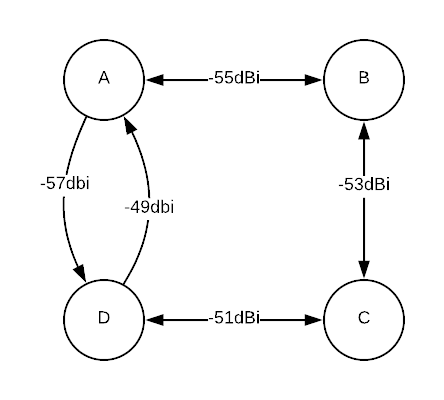
\includegraphics[width=8.5cm]{Images/gridlock.png} }}%
	\caption{Gridlock situation with agglomerative clustering}
	\label{fig:gridlock}
\end{figure}

Vanilla agglomerative clustering also does not facilitate an upper cluster size bound, albeit this would be a trivial modification to do. 
\subsection{K-Closest Neighbour Clustering}
\label{chap:kcn}
To resolve the problem discussed in the previous section, we will perform a little modification to agglomerative clustering. 
To separate it from agglomerative clustering, we will call it K-Closest Neighbour Clustering (KCNC). In this method, similar to agglomerative clustering, in the beginning there are an equal amount of  clusters as there are nodes. 
The difference is that instead of looking for pairs that are mutually close, each cluster will attempt to merge with the cluster that it itself observes as closest. The distance is defined by the same distance metric, observed signal strength. In short: the merge will always happen as long as the resulting cluster does not contain a higher node count than K.

\subsubsection{Description}
Each node begins by identifying itself as a member of a group that only contains itself. Let us call this group $a$.
Group $a$ loops through the radio readings of every member of its group, and picks the node with the highest observed -dBi value
to contact. Of course, in the beginning there is only one node in group $a$, hence in the first iteration this node's radio readings alone will decide which group to merge with. 

The neighbour node which we will call $B$, is the node that disturbs group $a$ the most. $B$ is a member of group $b$.
In other words, group $a$ wants to merge with group $b$ to create a larger group that contains node $B$.

A merge happens in the following way: the members of the two groups exchange information about all their member nodes and their radio readings and combine the information.
As the data is now identical for all the members of both groups and they can make identical choices it means that they are part of the same group. 

In our simulation this is as easy as combining two Group objects into one. A pseudocode sample of an implementation can be seen in \ref{fig:groupmerge}.

	\begin{figure}
		\tiny
		\begin{python}
allGroups = [];
K = 120;

for node in topology: //Initialize groups
	g = new Group()
	g.members.append(node)
	allGroups.append(g);

while True: //Run as long as there are changes
	changes = 0;	
	for group in allGroups: 
		groupMaxDbi = -INFINITE
		groupClosestNode = None

		for node in group:
			nodeMaxDbi = -INFINITE
			nodeClosestNode = None

			for neighbour in node.neighbours:
				if neighbour.dbi > nodeMaxDbi:
					nodeMaxDbi = neighbour.dbi
					nodeClosestNode = neigbour

			if (nodeMaxdbi > groupMaxDbi):
				groupMaxDbi = groupMaxDbi
				groupClosestNOde = nodeClosestNode:

		var groupToMergeWith = groupClosestNode.group
		if (length(group.members) + length(groupToMergeWith.members)) < K:
			var newGroup = new Group()
			newgroup.members = group.members + groupToMergeWith.members
			allGroups.append(newgroup)
			allGroups.remove(groupToMergeWith)
			allGroups.remove(group)
			changes = 1
	if (changes == 0):
		break
		\end{python}
			\caption{Pseudocode sample of how the K-Closest Neighbour Clustering runs in a simulated environment}
			\label{fig:groupmerge}
	\end{figure}



Merges can not always be accepted, else the group would eventually contain all nodes in the entire topology. That is why we define a maximum threshold for the amount of members a group can have, 
referred to as K. If the sum of members in two groups that wants to merge exceeds K, the merge is aborted and no changes are reported to have happened for either group. 
This means that the simulation algorithm converges when no groups remain that are small enough to merge with another.
 
\subsection{Simulations}
Figure \ref{fig:knearest}a shows the result of running the K-Closest Neighbour Clustering algorithm on a uniform distribution topology, while figures \ref{fig:knearest}b, \ref{fig:knearest}c, \ref{fig:knearest}d shows the resulting clusters after running it on topologies on cities and towns collected by WiGLE. The different node colors indicate different group memberships. For closer inspection,
the large scale images of each topology can be seen in appendix \ref{appendix:knn}.
\begin{figure}
		\centering
		\subfloat[Uniform]{{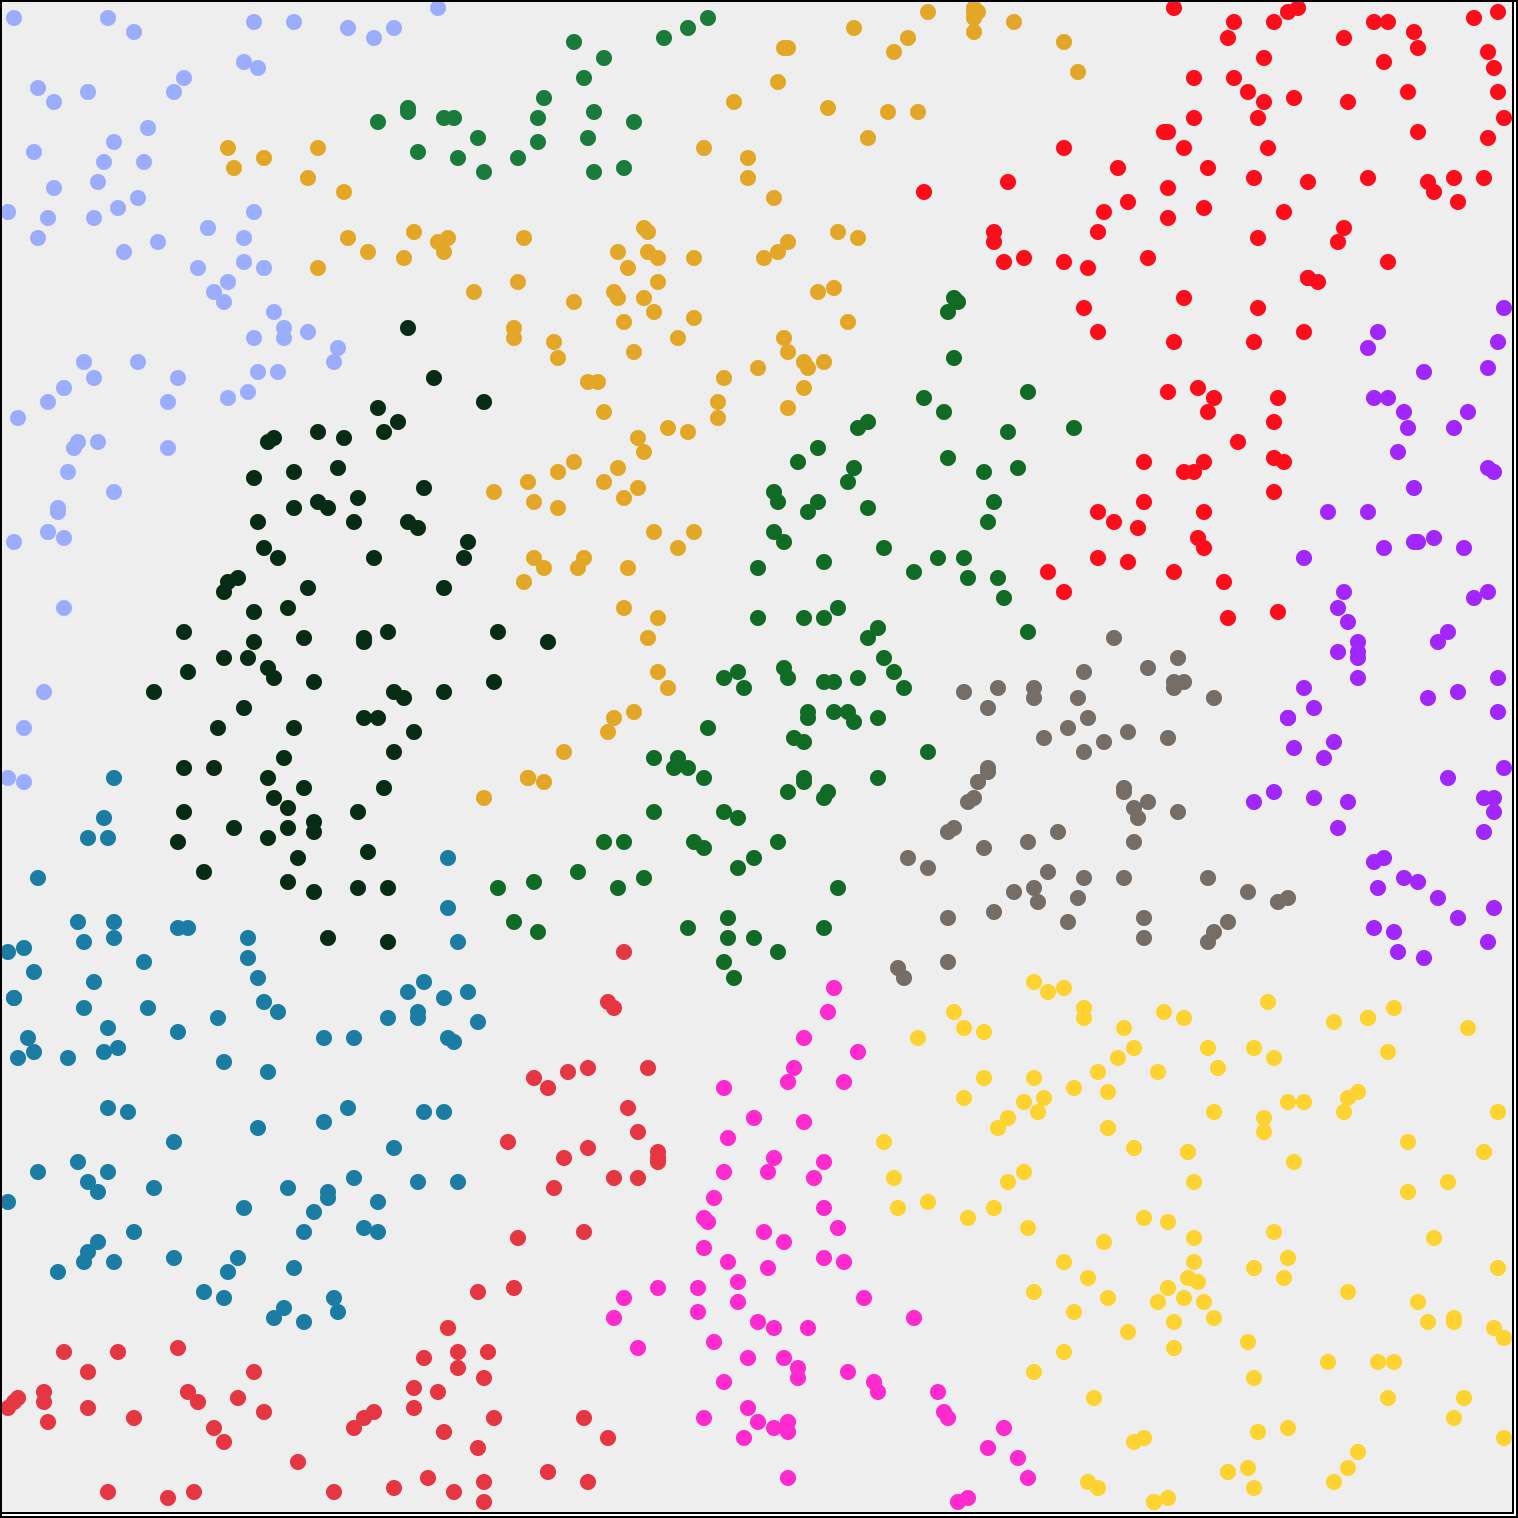
\includegraphics[width=4.5cm]{Images/computations/BASIC500x500_1000n.jpg} }}%
		\qquad
		\qquad
		\subfloat[Forks]{{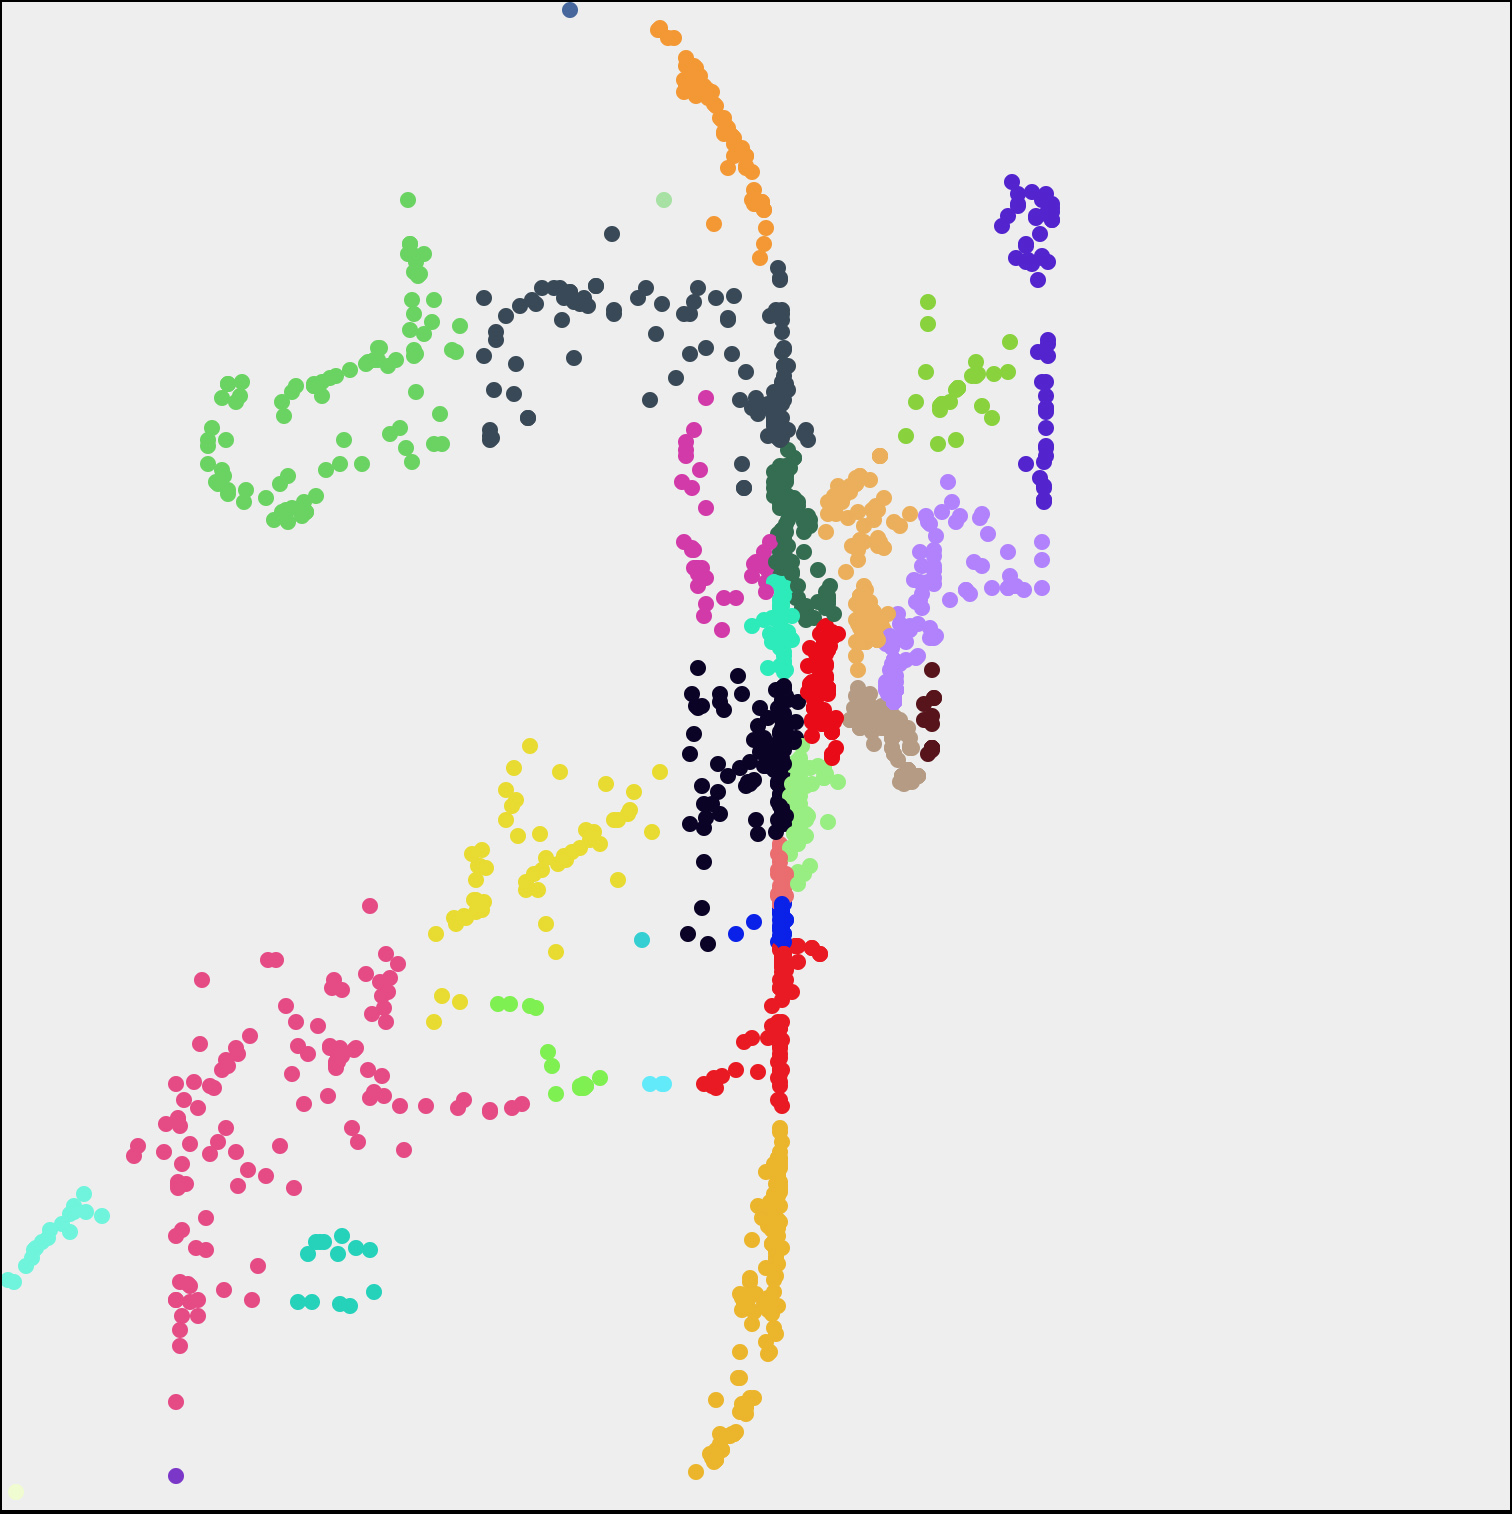
\includegraphics[width=4.5cm]{Images/computations/BASICForks.jpg} }}

		\subfloat[Lillehammer]{{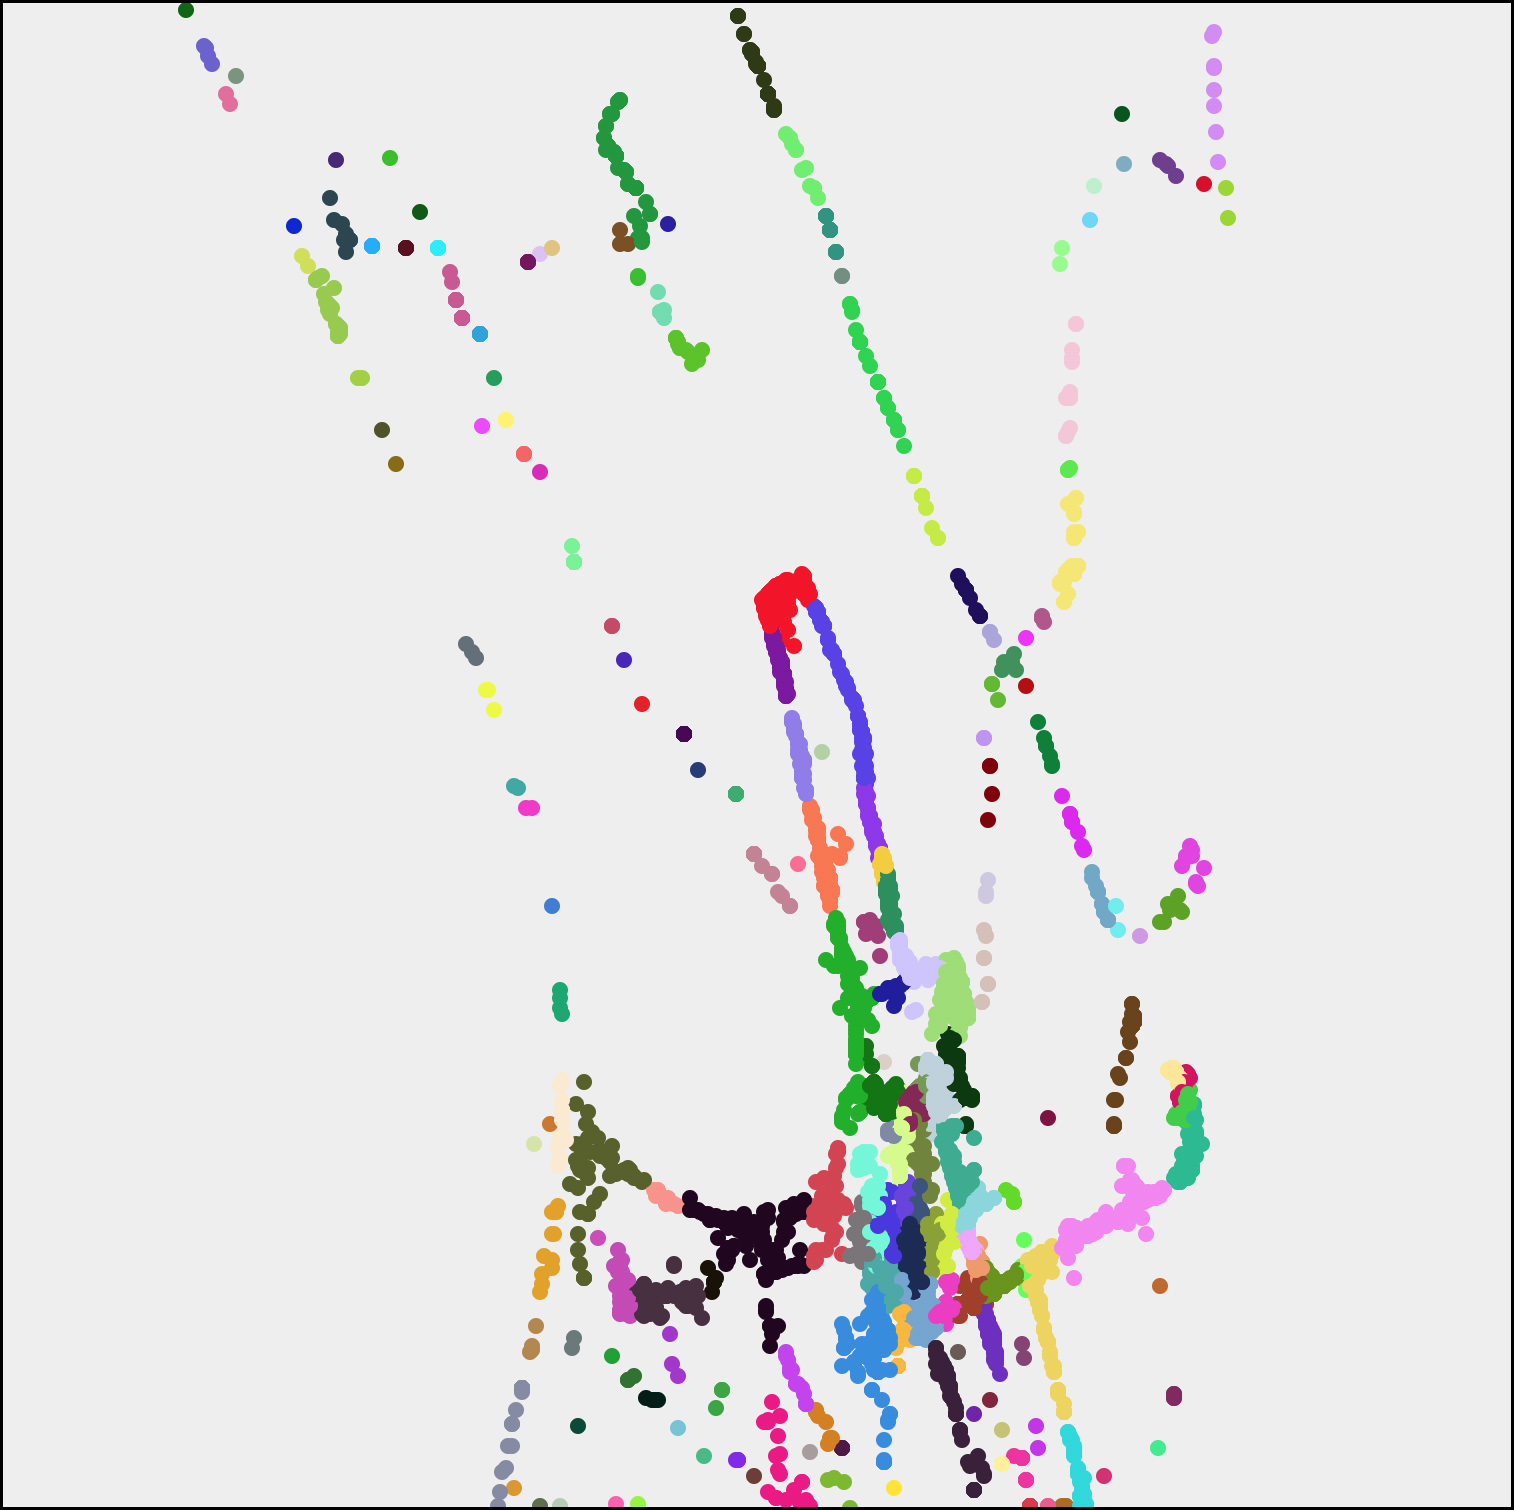
\includegraphics[width=4.5cm]{Images/computations/BASICLillehammer.jpg} }}%
		\qquad
		\qquad
		\subfloat[Tynset]{{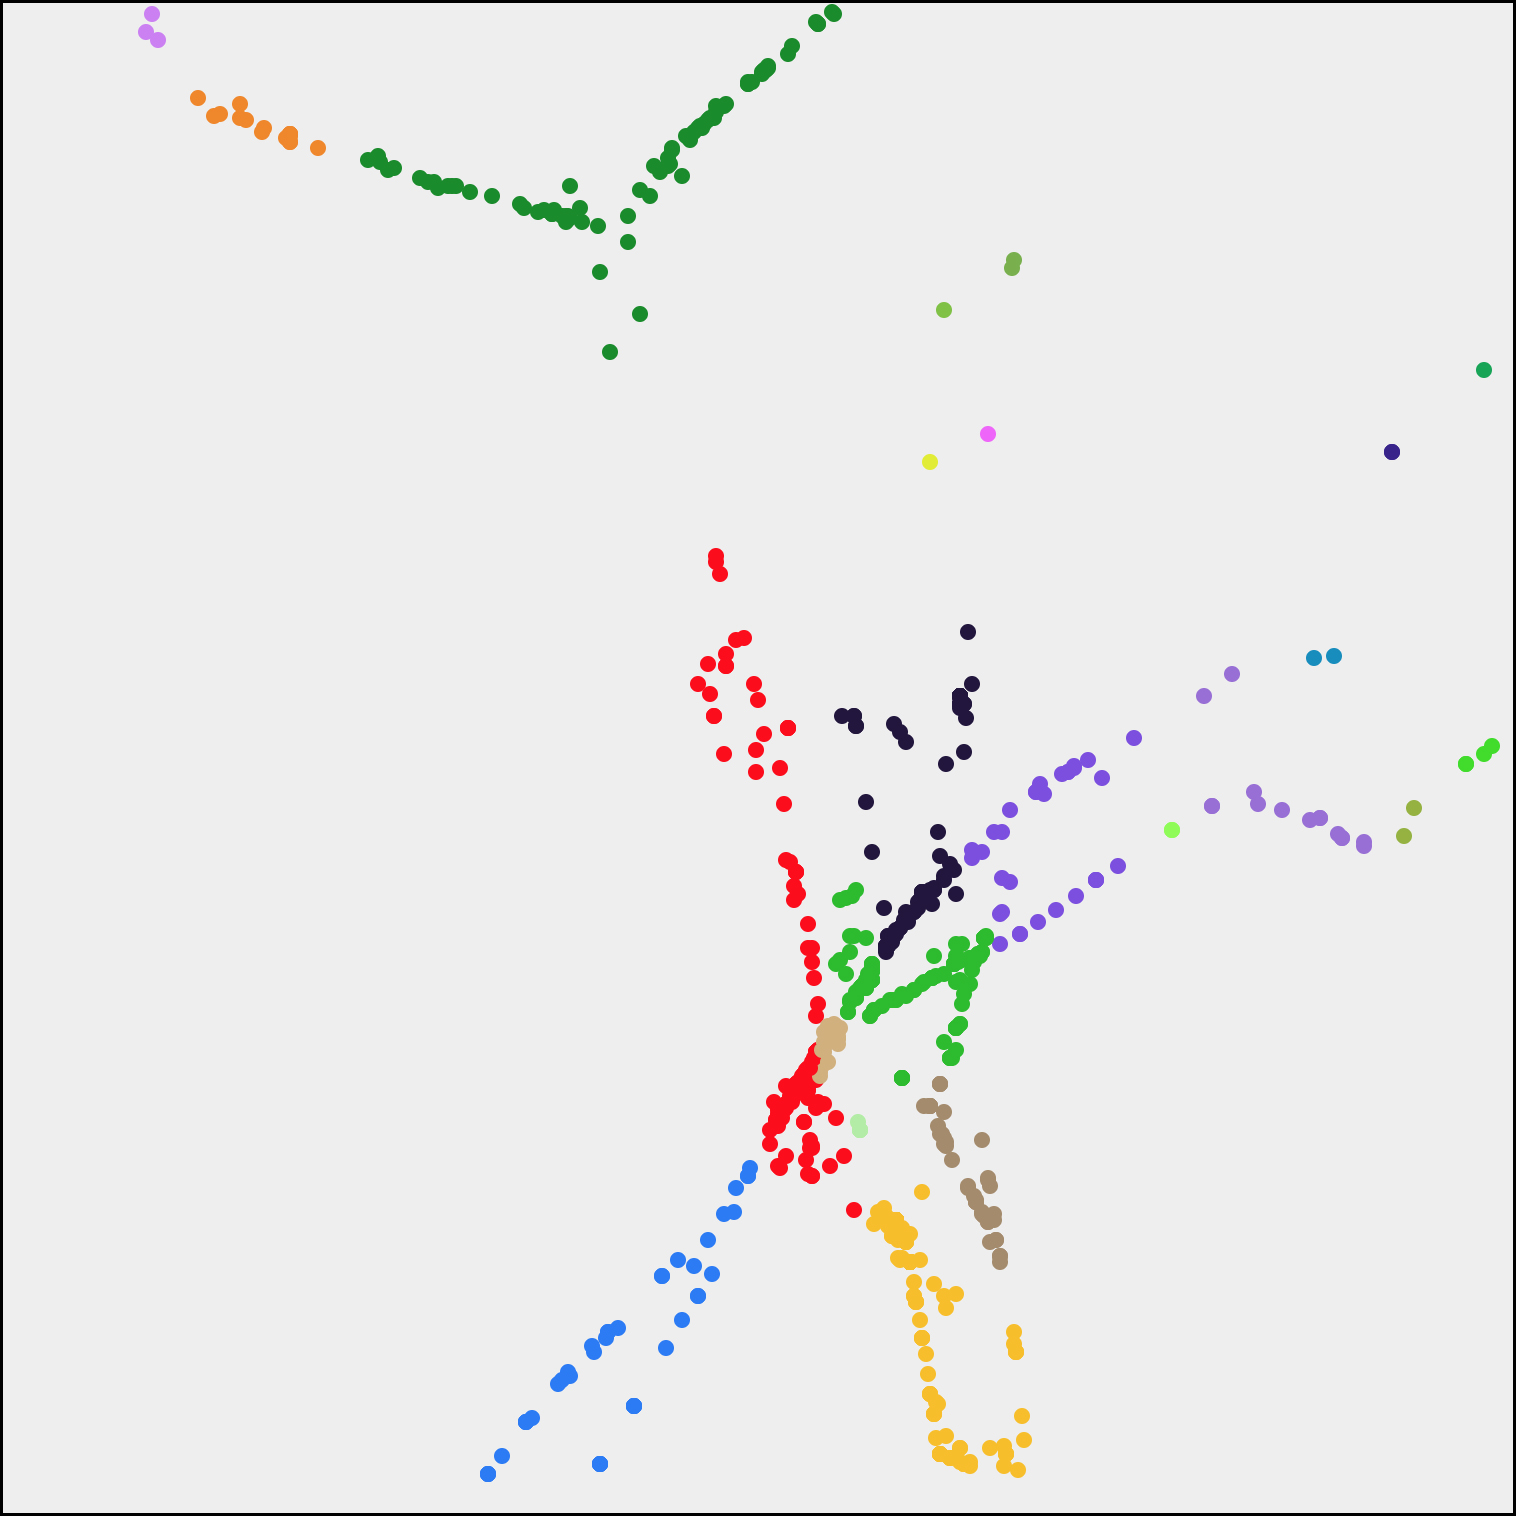
\includegraphics[width=4.5cm]{Images/computations/BASICTynset.jpg} }}%
		\caption{K-Closest Neighbour Clustering on different topologies}%
		\label{fig:knearest}%
\end{figure}

\subsection{Observations}
By looking at the results of the simulations of the K-Closest Neighbour Clustering it is obvious that clusters are created that contains the nearest nodes.
Even in the more chaotic topologies as Lillehammer there are distinct clusters that encompasses the most impactful nodes. However, there are two obvious problems with this algorithm
which makes it unsuitable:

\begin{itemize}
	\item In contrast to agglomerative clustering, our K-Closest Neighbour Clustering algorithm does not care if the closest distance between the groups is pairwise mutual. This
		might lead to one group $a$ merging into another group $b$, even while $b$ has another neighbouring group $c$ that lies closer. If the maximum size K is reached during the merge of
		$a$ and $b$,  the resulting group will never be able to merge with $c$ even though that would have given a better cluster. This violates requirement 4 from \ref{chap:requirements}. 
	\item Once a cluster reaches the maximum size K, there is no possibility for any other nodes to join the cluster.
		In the simulation of static topologies that might work, but in a real world scenario access points may turn on randomly and be located in the middle of an already existing cluster.
		With this algorithm alone there is no way to handle this event, and the new node could not become a member of the cluster that surrounds it. This violates requirement 2 from \ref{chap:requirements}.
\end{itemize}
In the next section we will look at how we can use group splitting to offer a solution for these problems.

\section{K-means splitting}
In this section the concept of group splitting will be introduced. Group splitting might improve the K-Closest Neighbour Clustering algorithm suggested in the previous section.

\subsection{Group splitting hypothesis}
An implication created by letting one cluster merge with another without knowing if the merge is mutually beneficial, is that not all merges will be optimal.
A way to increase the likelihood of a group ending up with the neighbouring nodes that impacts each other severely would be to accept merges that result in groups larger than K, the maximum size. 
The group would be too large, but more likely to have the opportunity to merge with the nodes of highest impact. To reduce the group size back to K,
the least impactful nodes would have to be kicked out of the group. This is what we call group splitting. A simplified illustration of the basic concept is shown in figure \ref{fig:splitting},
where the maximum group size is 2 and two neighbouring nodes join to reach the maximum group size. A third, more impactful node appears, and is included in a transient group
before the least disturbing node is kicked out to get the group size back to K. 

\begin{figure}
	\centering
		\subfloat[Two neighbouring nodes]{{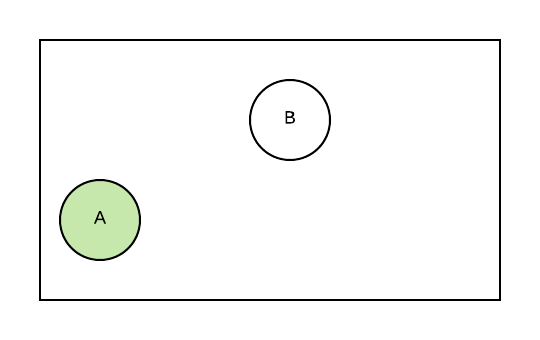
\includegraphics[width=5cm]{Images/mergestep1.png} }}%
		\qquad
		\qquad
		\subfloat[A and B merges. A third node appears]{{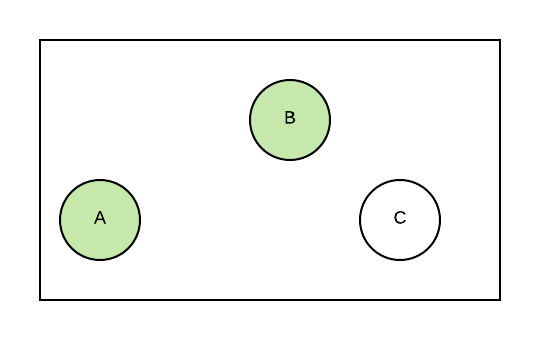
\includegraphics[width=5cm]{Images/mergestep2.png} }}%

		\subfloat[All nodes joined in transient group]{{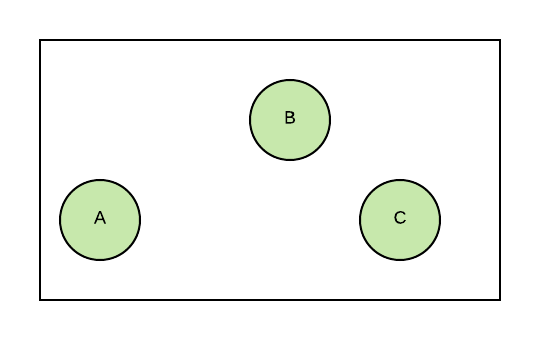
\includegraphics[width=5cm]{Images/mergestep3.png} }}%
		\qquad
		\qquad
		\subfloat[Splitting to reduce group size]{{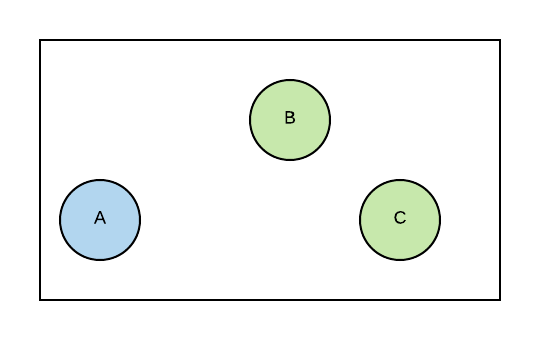
\includegraphics[width=5cm]{Images/mergestep4.png} }}%
		\caption{Simplified illustration of the idea behind splitting. K = 2}%
		\label{fig:splitting}%
\end{figure}

\subsection{K-means splitting}
K-means clustering is not directly applicable to solve the clustering challenge in this thesis. The simple reason being the distributed nature of
the nodes and groups. Indeed, a vanilla implementation of K-means requires an extensive overview of the surrounding, if not entire, network topology.
The groups are so far limited to knowing about their members and their neighbours. It would also be hard to choose a suitable K. 

Nonetheless, K-means could still potentially help create better groups. Let us consider the following.
By extending the K-Closest Neighbour Clustering so groups are allowed to merge into a transient group if it exceeds the given maximum size.
The purpose of the large transient group is to identify the biggest gap between nodes, and split the group in two new groups with
$count(nodes) < maxsize$. If we set the K-means variable K, to $K=2$, K-means can be used to identify where the transient group should be split to create two more connected clusters. 

Randomly picking two nodes to be centroids could lead to undesirable results where the two resulting groups are fundamentally different from the original ones.
Recall that the purpose of the split is to reevaluate the division line between the groups and see if K-means can achieve a better split, not create two entirely new clusters.
There already exists two independent clusters before the split. The centroids of these clusters can be pre-calculated before merging, and be used to bootstrap K-means with two non-randomly chosen
centroids.
If the distance between the most interfering nodes is lower after applying the K-means split, the new groups are applied. On the other hand, if the distance is shorter
(meaning a less optimal cut is found) the original groups are restored. As the bootstrapped position of the centroids is planned and not random,
the result is deterministic and the algorithm does not have to be run more than one time to get the result. 


\subsection{Simulations}
The results of simulating the group creation with K-means splitting implemented can be seen in figure \ref{fig:kmeans} (see 
appendix \ref{appendix:kmeanssplit} for full size images). The groups clearly look very similar to those we computed in \ref{fig:knearest}, but in some places there are some major differences. This is where splits have happened. A comparison of the two algorithms executed on the same section of Tynset's town centre can be seen in figure \ref{fig:kmeanscomparison}, and another
comparison of a section of the uniform distribution can be seen in figure \ref{fig:kmeanscomparisonuniform}. 

\begin{figure}
	\centering
		\subfloat[Uniform]{{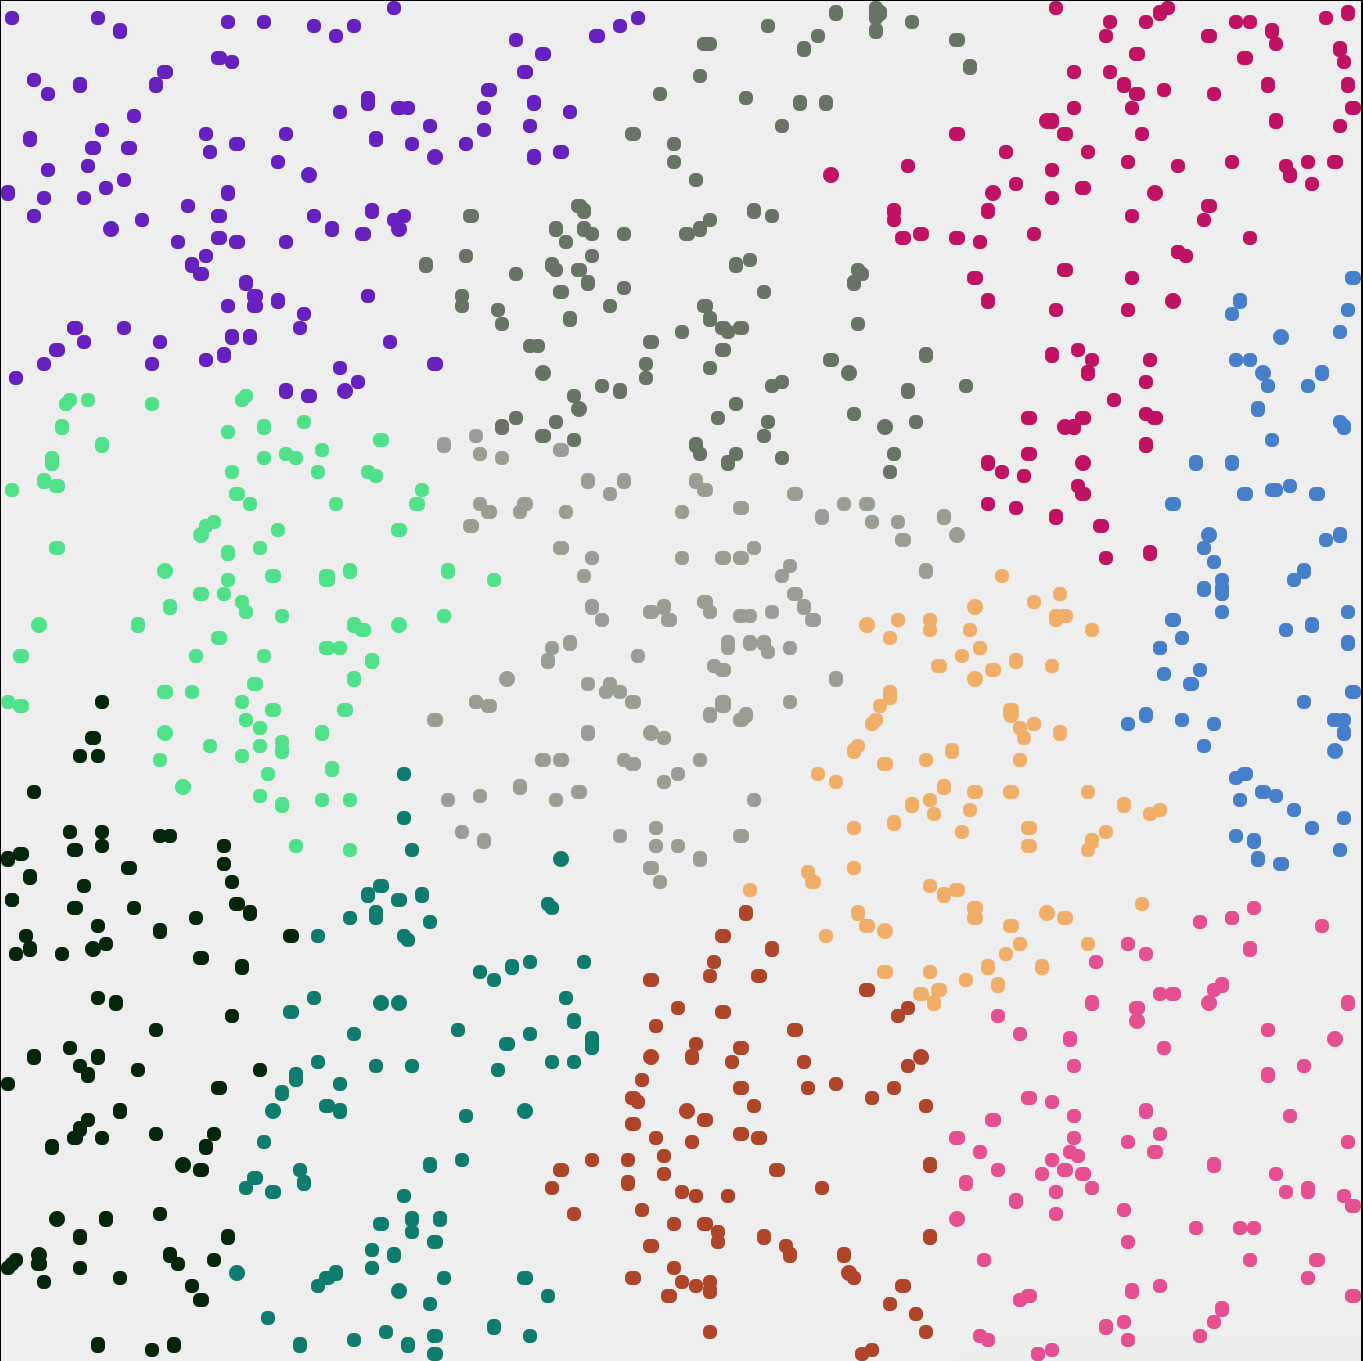
\includegraphics[width=5cm]{Images/computations/KMEANS500x500_1000n.jpg} }}%
		\qquad
		\qquad
		\subfloat[Forks]{{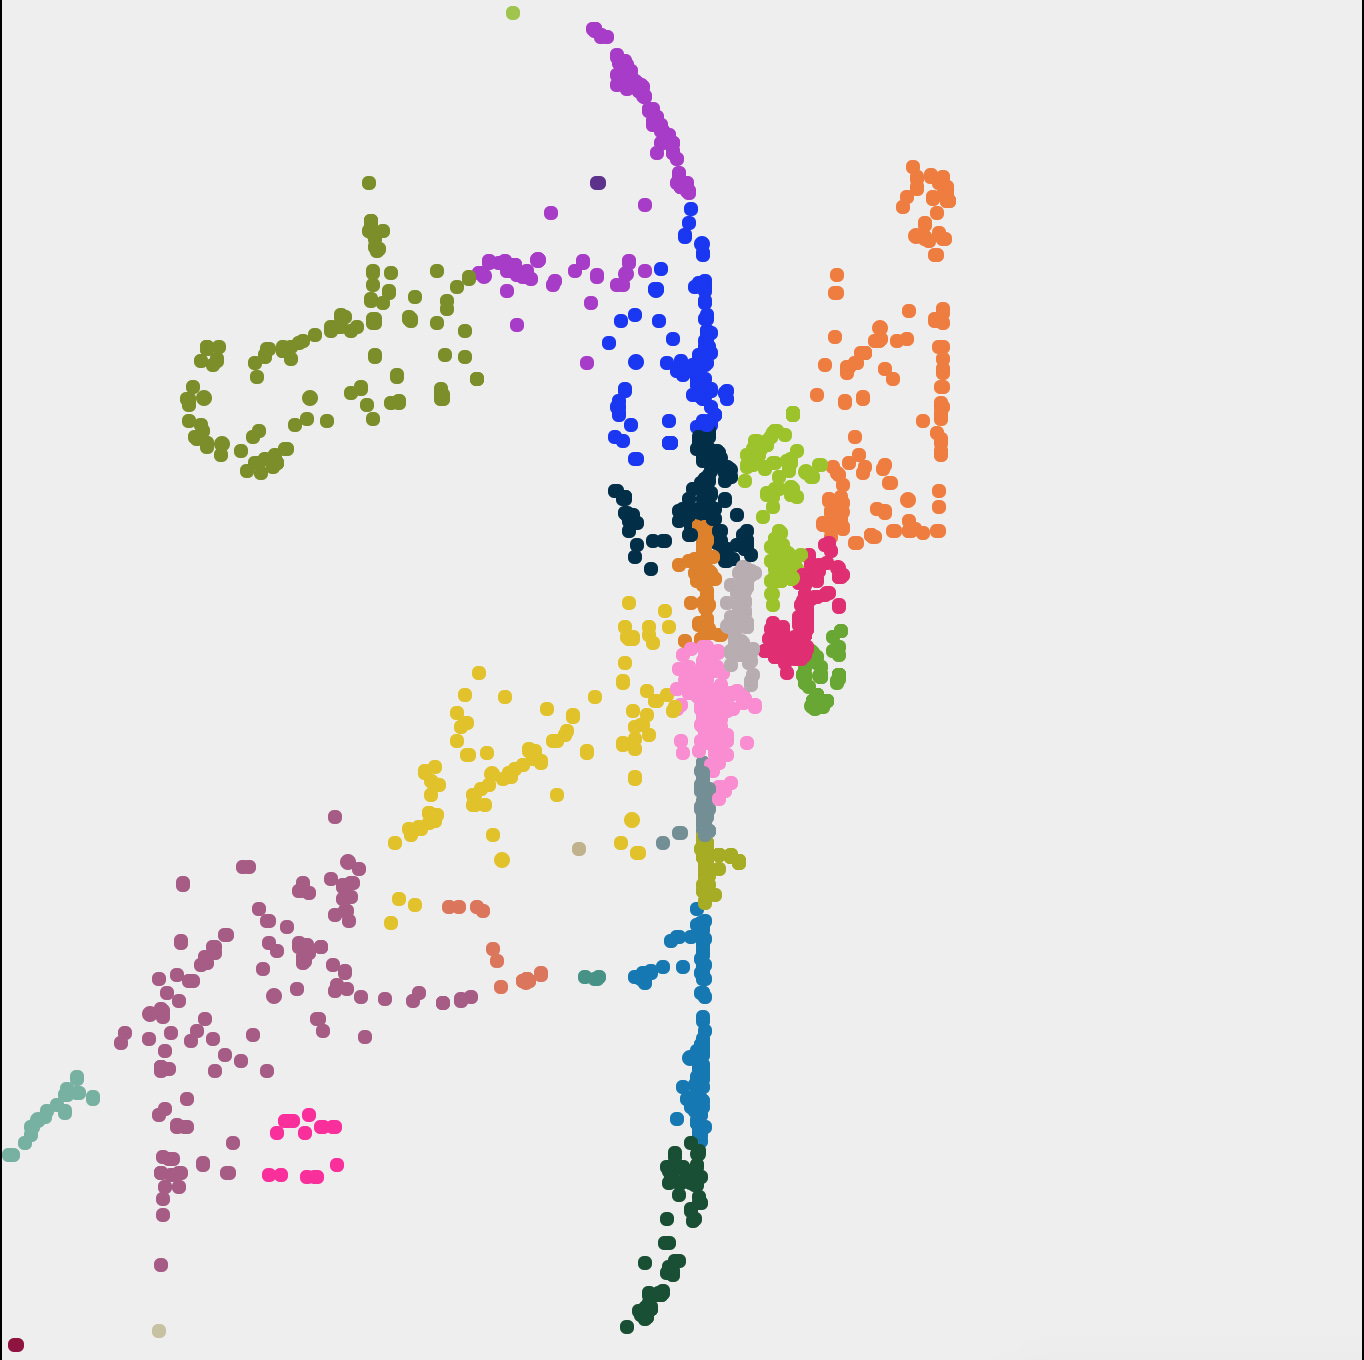
\includegraphics[width=5cm]{Images/computations/KMEANSForks.jpg} }}%

		\subfloat[Lillehammer]{{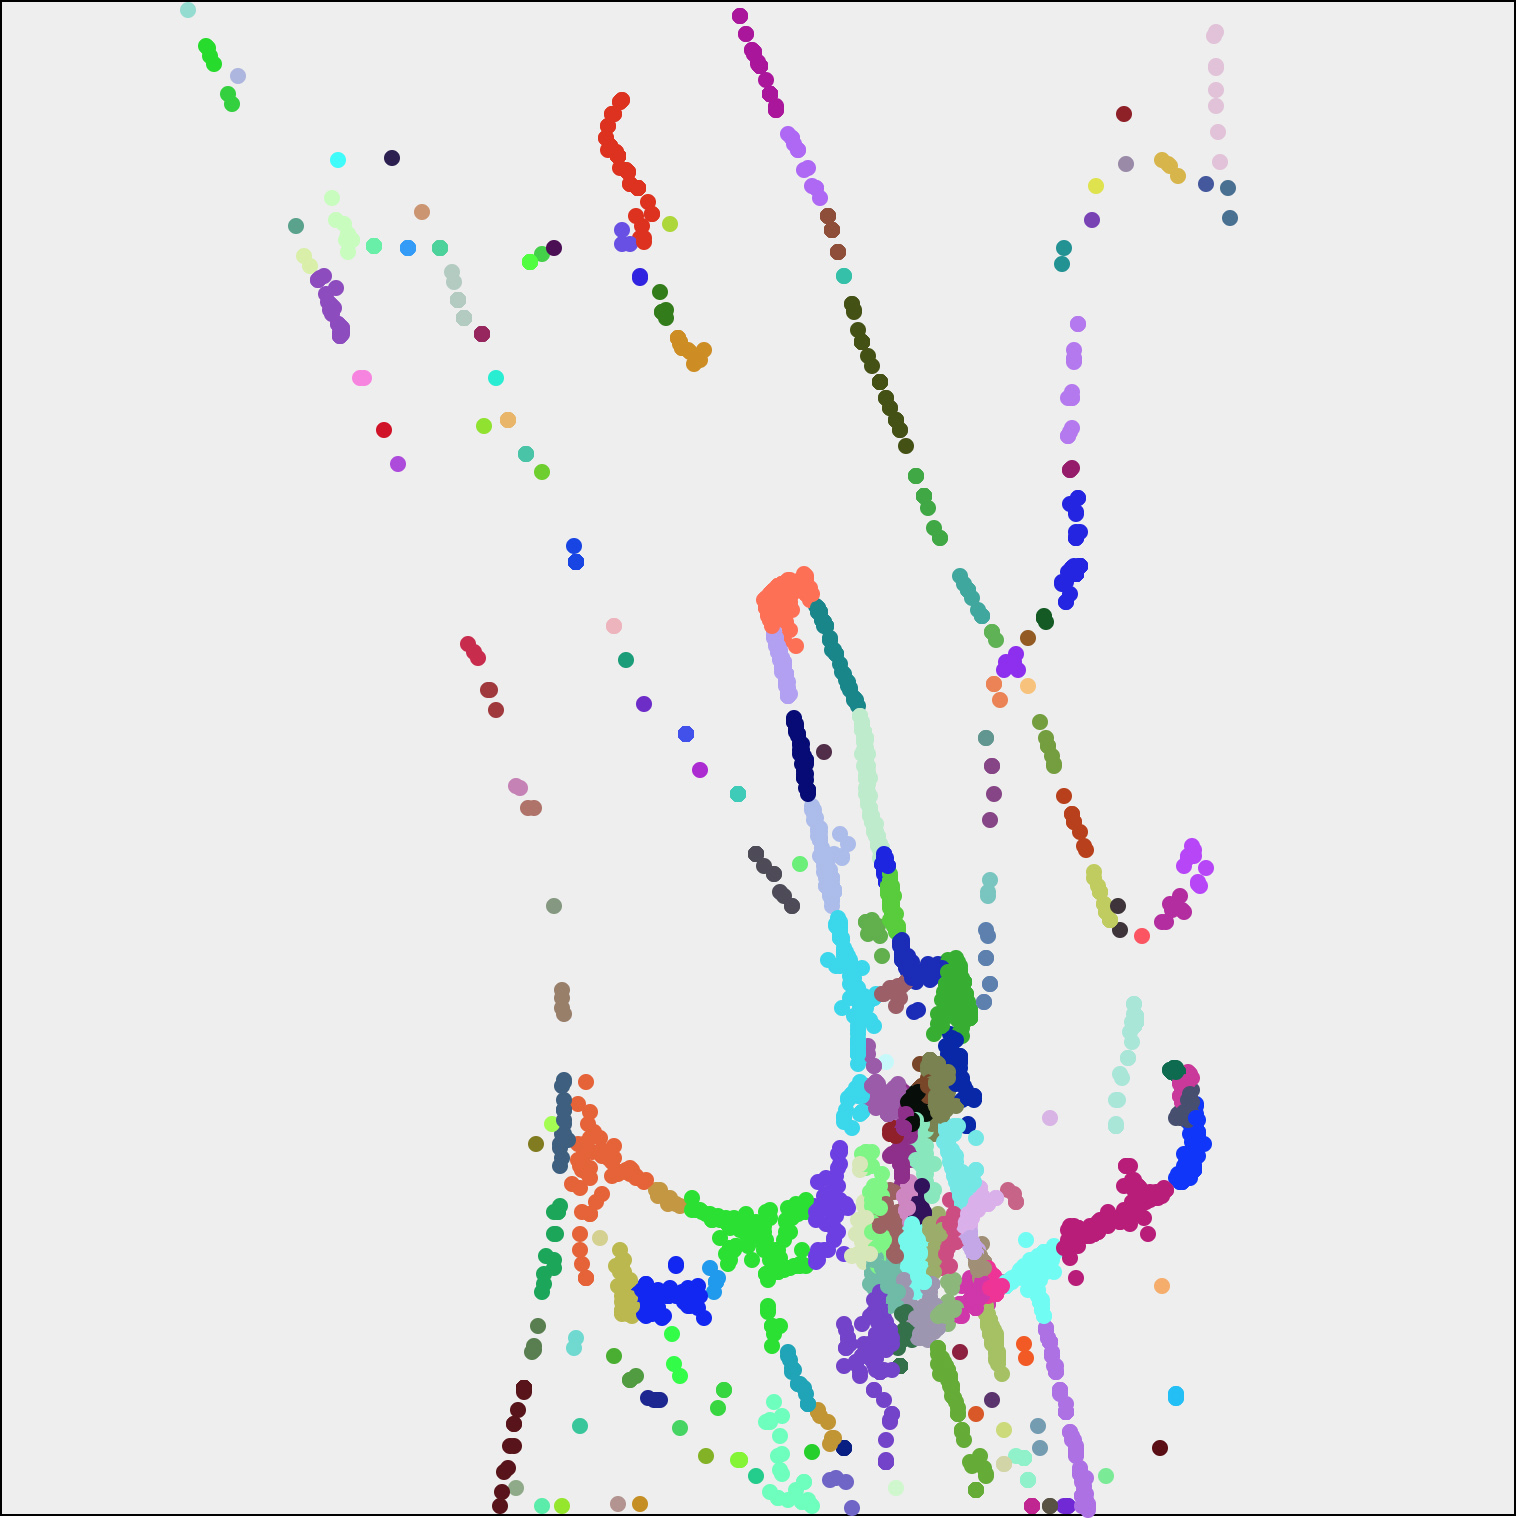
\includegraphics[width=5cm]{Images/computations/KMEANSLillehammer.jpg} }}%
		\qquad
		\qquad
		\subfloat[Tynset]{{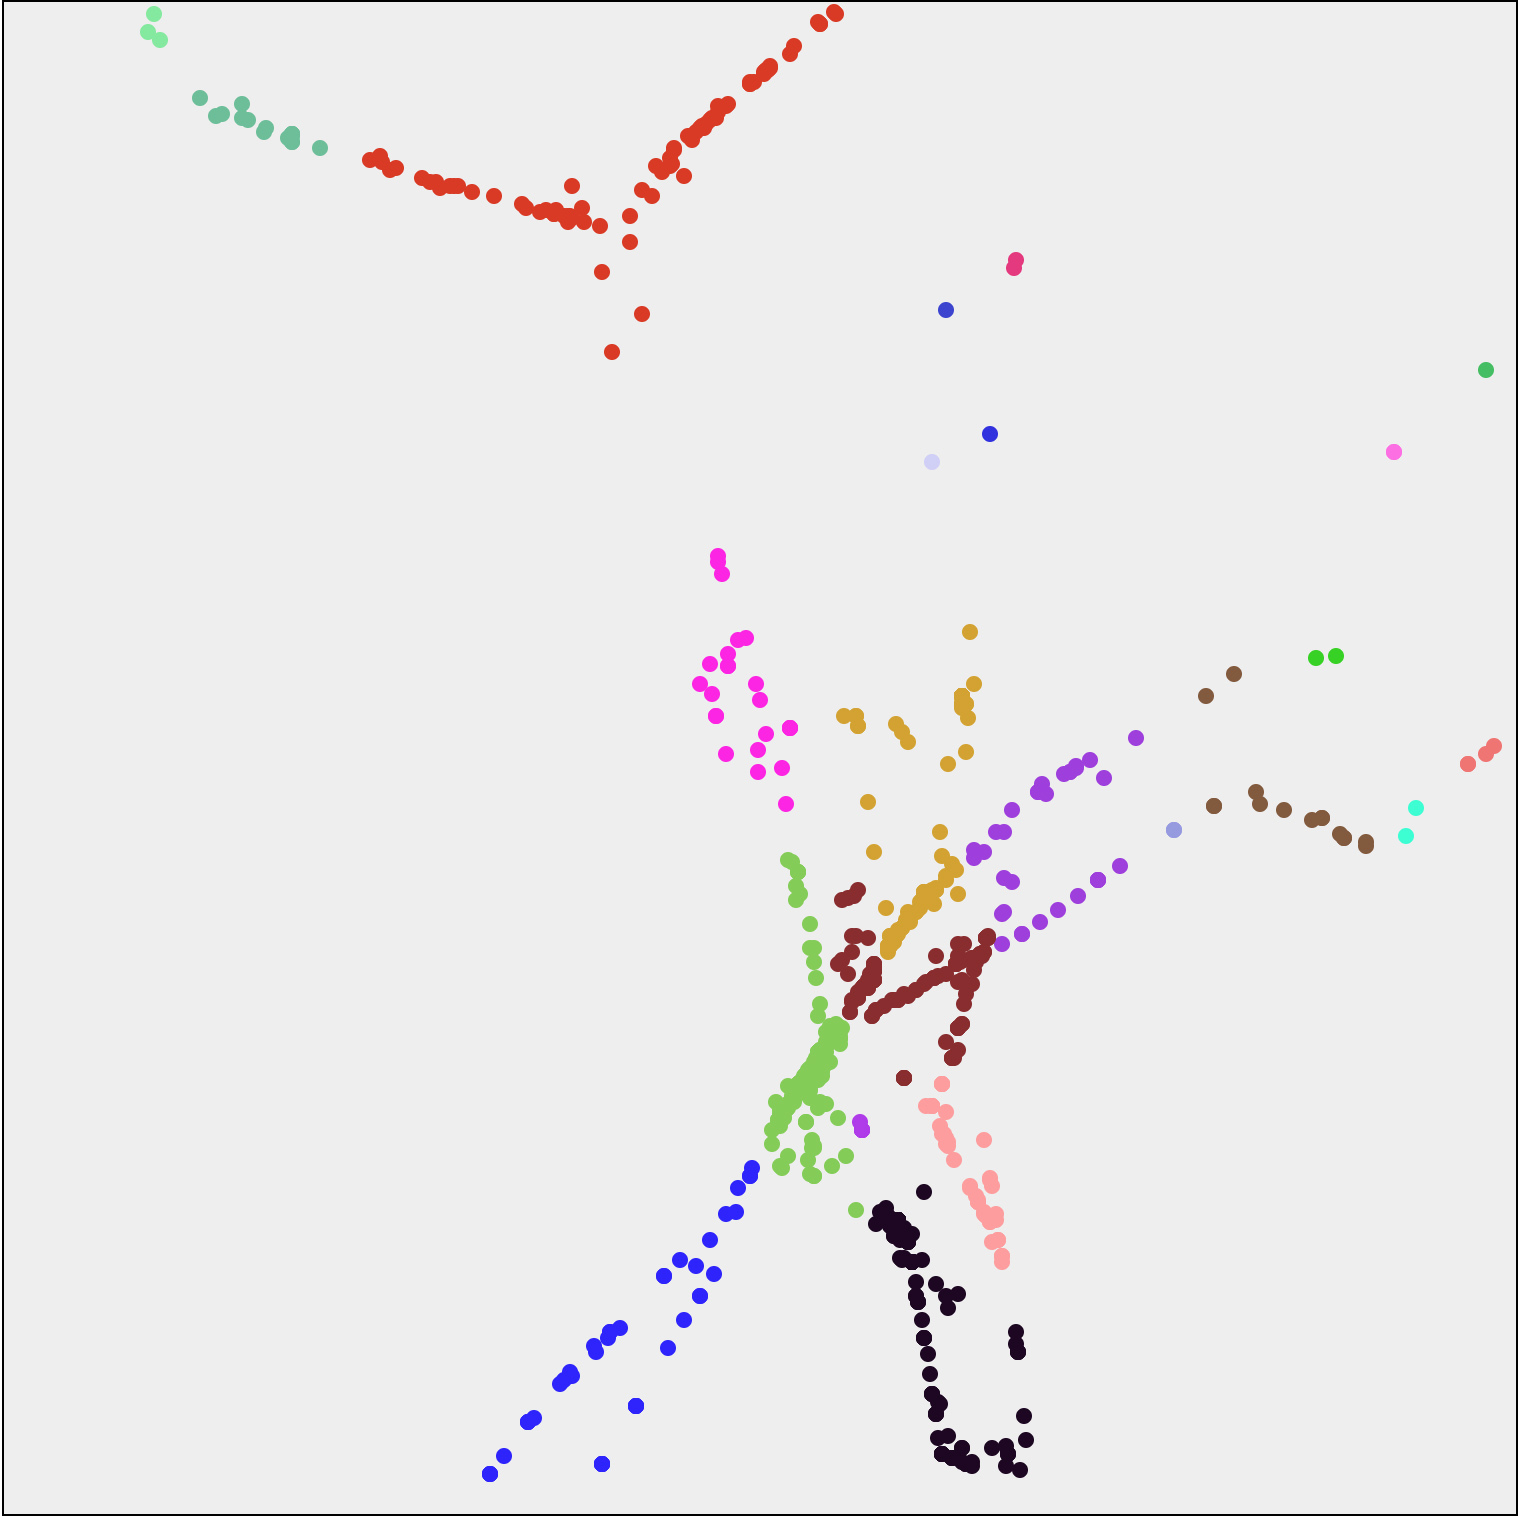
\includegraphics[width=5cm]{Images/computations/KMEANSTynset.jpg} }}%
		\caption{K-means splitting on different topologies}%
		\label{fig:kmeans}%
\end{figure}

\begin{figure}
	\centering
		\subfloat[Without K-means splitting]{{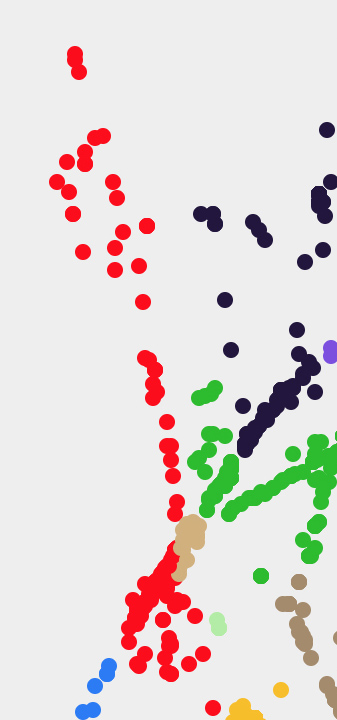
\includegraphics[width=2.5cm]{Images/computations/TynsetNear.jpg} }}%
		\qquad
		\subfloat[With K-means splitting]{{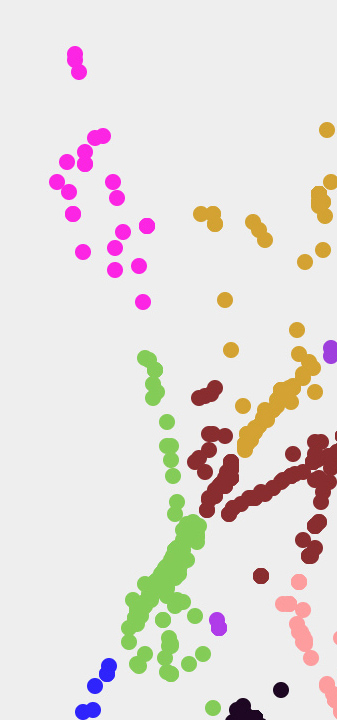
\includegraphics[width=2.5cm]{Images/computations/TynsetNearKmeans.jpg} }}%
		\caption{Comparison with and without K-means splitting on Tynset}%
		\label{fig:kmeanscomparison}%
\end{figure}

\subsection{Observations}
There is little doubt that K-means splitting improves upon the original algorithm, especially when splits are only accepted when the maximum interference between groups is reduced after the split.
Even though the clusters in a static environment is slightly improved, the most important use-case for K-means splitting is under the introduction of new nodes to an environment
where all groups have converged. Where in the unmodified K-Closest Neighbour Clustering algorithm there was no specific way to handle a new node in an environment of saturated groups,
with K-means splitting eventually new groups will be formed on the basis of the updated topology. The weakness of this approach is how ill suited it is to run in a distributed environment.
It is trivial to simulate splits using K-means, as during a simulation the absolute coordinates of the nodes in the group are accessible. This is information unavailable for nodes under
real circumstances - the only available information is the approximate point-to-point distance inferred from the signal strength scans.
Hence some major adaptions would have to be made to get this to work in an implementation.
One way to realize the algorithm would be to select a physical node as centroid instead of a virtual point. All nodes in sensing range of the surrounding area of
the centroid node would report the distance to the centroid to their n-hop neighbour using an overlay network to communicate internally in the group. The other nodes could
then figure out their approximate distance to the centroid. It is unknown if such an approach would be accurate enough to work, or have a complexity that is conceivable to implement.  

\begin{figure}
	\centering
		\subfloat[Without K-means splitting]{{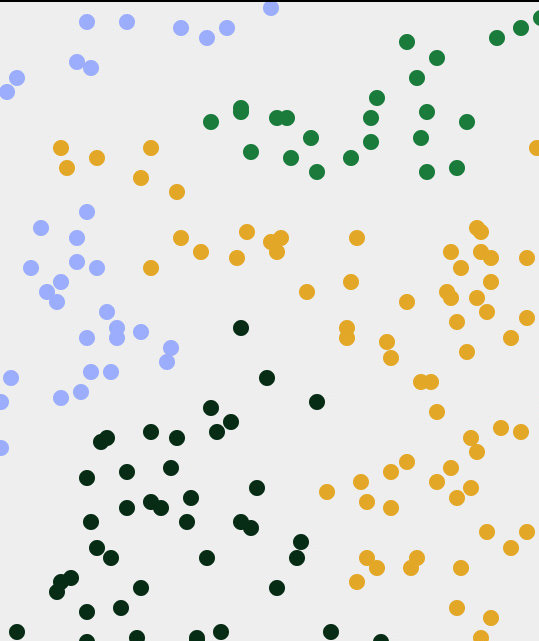
\includegraphics[width=4cm]{Images/computations/500x5000Near.jpg} }}%
		\qquad
		\subfloat[With K-means splitting]{{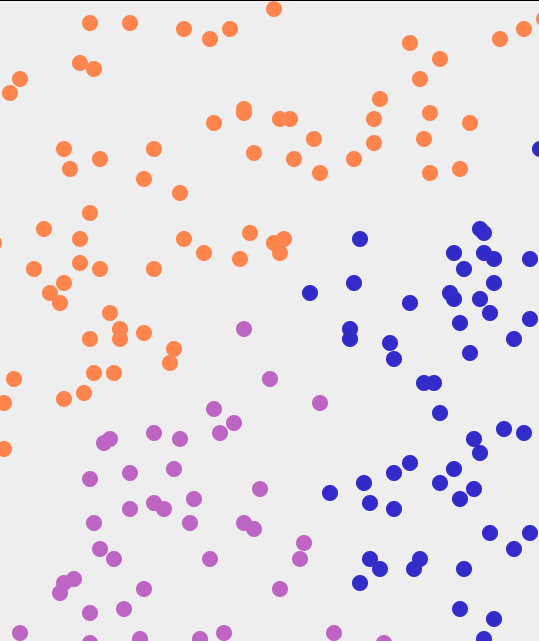
\includegraphics[width=4cm]{Images/computations/500x5000NearKmeans.jpg} }}%
		\caption{Comparison with and without K-means splitting on uniform distribution}%
		\label{fig:kmeanscomparisonuniform}%
\end{figure}


\section{Minimum Cut Splitting}
\label{chap:mincut}
In this section we will consider another approach to group splitting, namely the graph theory algorithm for finding a minimum cut in a directed graph. 

\subsection{Minimum cut}
The core concept of the minimum cut algorithm is to find a way to cut a directed graph so that a source node is completely separated from a sink node, while cutting over edges 
whose weights adds up to a sum which is as low, or minimal, as possible \cite{chinneck}.

The minimum cut is often referenced in the context of the max-flow min-cut theorem, which states that the maximum flow of a directed graph is equal to the capacity of the minimum cut.
The capacity of the minimum cut is equal to the sum of the weight of the edges the cut runs through. In 1956 Delbert R. Fuelkerson and Lester R.
Ford proposed a method for finding the minimum-cut \cite{ford1956} in a flow network, now called the Ford-Fuelkerson method. The method was extended by the Edmonds-Karp algorithm \cite{Edmonds} which is identical, except that is specifies that a breadth-first search should be used for the augmented-path stages in the algorithm, whereas in Ford-Fuelkerson this is unspecified (hence being called
a method, and not an algorithm).

The implementation of minimum cut that will be used in this section is a part of the NetworkX \cite{NetworkX} python package for manipulation of complex networks.

\subsection{Using minimum cut for group splitting}
Minimum cut can be used for group splitting by identifying the least connected partitions of a group. If a node, or a partition of the group, is connected to the rest of the group
through one or more links which are weaker than the strongest link to a neighbouring group, the partition can be excluded from the group to allow for a merge with the neighbouring group. 


\begin{figure}
	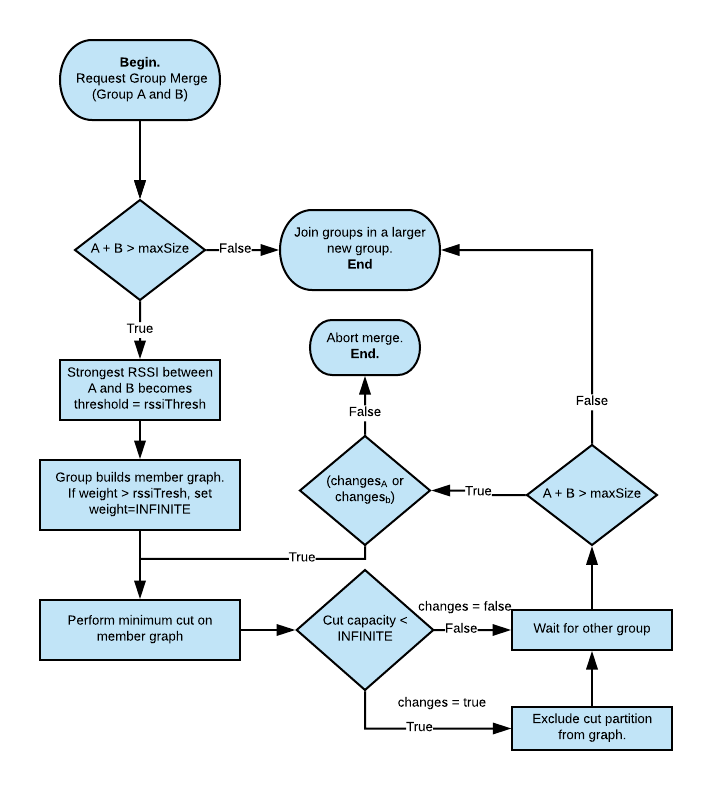
\includegraphics[width=\textwidth]{Images/mincutflow2.png}
		\caption{Flowchart of the minimum cut implementation for splitting}%
		\label{fig:mincutflow}%
\end{figure}


	\begin{figure}
		\tiny
		\begin{python}
			def findCutAndPartition(G, sink):
				minCutCapacity = 99999 #Initiated to infinite (or a very high number)
				minCutPartition = [] #Partition initially empty
				for source in G.nodes_iter():
					if source == sink: #Source and sink should not be the same
							continue
					cut, partition = nx.minimum_cut(G, source, sink)
					if (cut >= 99999): #If cut is too high (infinite), dont keep
							continue
					if cut < minCutCapacity:
							minCutCapacity = cut;
							#Identify which partition is to be separated form the grapzh
							if sink in partition[0]:
									minCutPartition = partition[1]
							elif sink in partition[1]:
									minCutPartition = partition[0]

				for n in minCutPartition: #Remove nodes from graph
							G.remove_node(n)
				return list(minCutPartition);
		\end{python}
		\caption{Pseudocode of the minimum cut stage of the splitting}
		\label{fig:pseudocut}
	\end{figure}


To utilize minimum cut as a mechanism for splitting, the groups have to be treated as directed graphs. While the data structure of the networks in the implementation is not
originally designed for graph operations, the nature of the nodes with its neighbour lists and signal strength metrics certainly can be treated as a graph. Meaning that each node's neighbour list contains
its outgoing edges, while the belonging signal strength value is the weight of the edge. In contrast to the K-means splitting implementation, the minimum cut implementation does not require
a larger transient group. Instead the groups have to negotiate to know when a split can be confirmed. A flowchart illustration of the simulation implementation can be seen in figure \ref{fig:mincutflow}, showing the steps which are more closely described below. 

\begin{enumerate}
	\item Two groups $A$ and $B$ wants to merge, their combined size is larger than the specified group $maxSize$. The measured maximum value of signal strength between nodes in the two different
		groups $A$ and $B$ is called $rssiThresh$. 
	\item The groups independently build a graph of their current state, using the signal strength values as weights on edges to neighbouring nodes. In the simulation implementation this is done using the NetworkX graph.
	\item Each edge in the graph where the weight is larger than  $rssiThresh$, gets a new weight = \verb|INFINITE|.
	\item The groups independently perform minimum cut multiple times. In the simulation implementation this is done with a call to the library function \newline \verb|minimum_cut(G, s, t)|,
		where $G$ is the graph, $s$ source and $t$ is the sink. To find the best partition to exclude from the graph, the  sink node is always the node which lies closest to the other group,
		while the source node changes for each call to minimum cut. When all nodes, except for the sink, have been sources in the minimum cut algorithm, this step is finished. The cut
		which has the lowest capacity of all performed cuts is stored along with the partition of this cut. 
	\item The partition which does not contain the sink node is excluded from the graph, however if this partition is empty it means there exists no suitable cuts in the group which are less beneficial than the addition of another group. 
	\item The groups $A$ and $B$ check if the combined number of nodes exceeds $maxSize$. If the node number is still too high, repeat step 4 provided that there were any 
		exclusions in the graphs in the previous run. If there are no exclusions in either group, there exists no cut that can bring the combined group size down to desired size, and the
		merge has to be aborted. 
\end{enumerate}

The pseudocode for step 4-5, referred to as the \verb|findCutAndPartition| procedure in the flowchart of \ref{fig:mincutflow}, can be seen in \ref{fig:pseudocut}.  

For a detailed step by step illustration describing how a split happens in a topology where a split would be beneficial, see figure \ref{fig:mincutstep}. 
\begin{figure}
	\centering
		\subfloat[Two groups are initially too large to merge. A split is going to be attempted. ]{{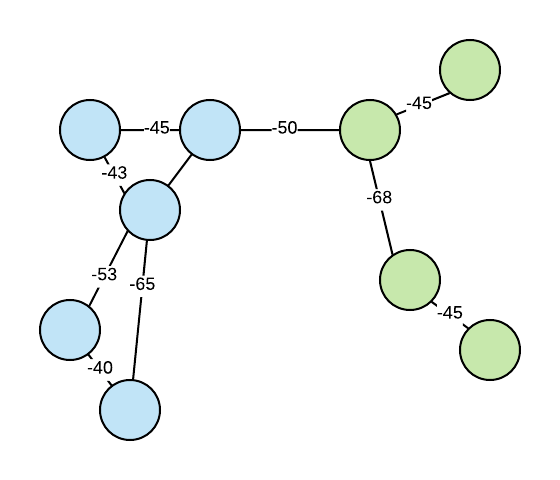
\includegraphics[width=7cm]{Images/mincutstep1.png} }}%
		\qquad
		\subfloat[Both groups identify edges which should not be cut, marked by an infinite edge weight]{{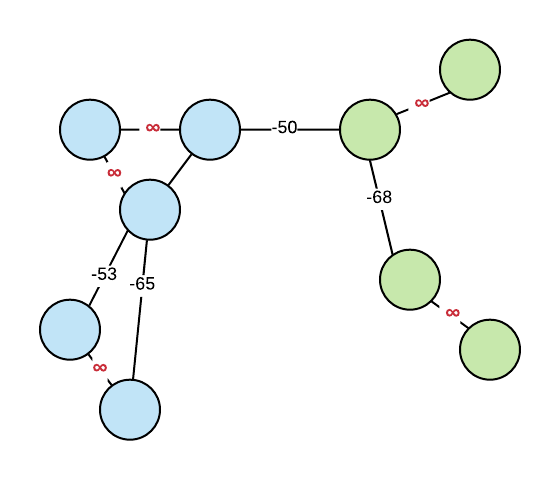
\includegraphics[width=7cm]{Images/mincutstep2.png} }}%
		
		\subfloat[The groups excludes the partitions with the lowest capacity cuts]{{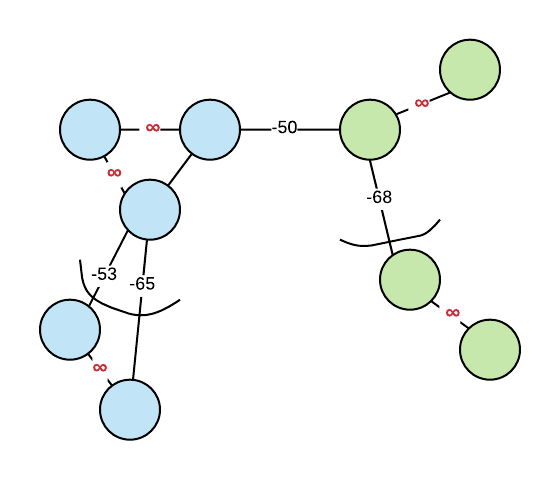
\includegraphics[width=7cm]{Images/mincutstep3.png} }}%
		\qquad
		\subfloat[The number of members of the groups combined is now lower than maximum size, and the merge is succesful]{{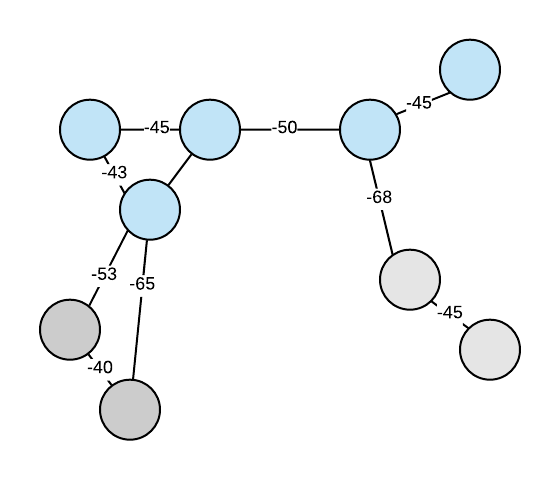
\includegraphics[width=7cm]{Images/mincutstep4.png} }}%
		\caption{Minimum cut illustration with group maximum size set to 5}%
		\label{fig:mincutstep}%
\end{figure}


\begin{figure}[t!]
	\centering
		\subfloat[Uniform]{{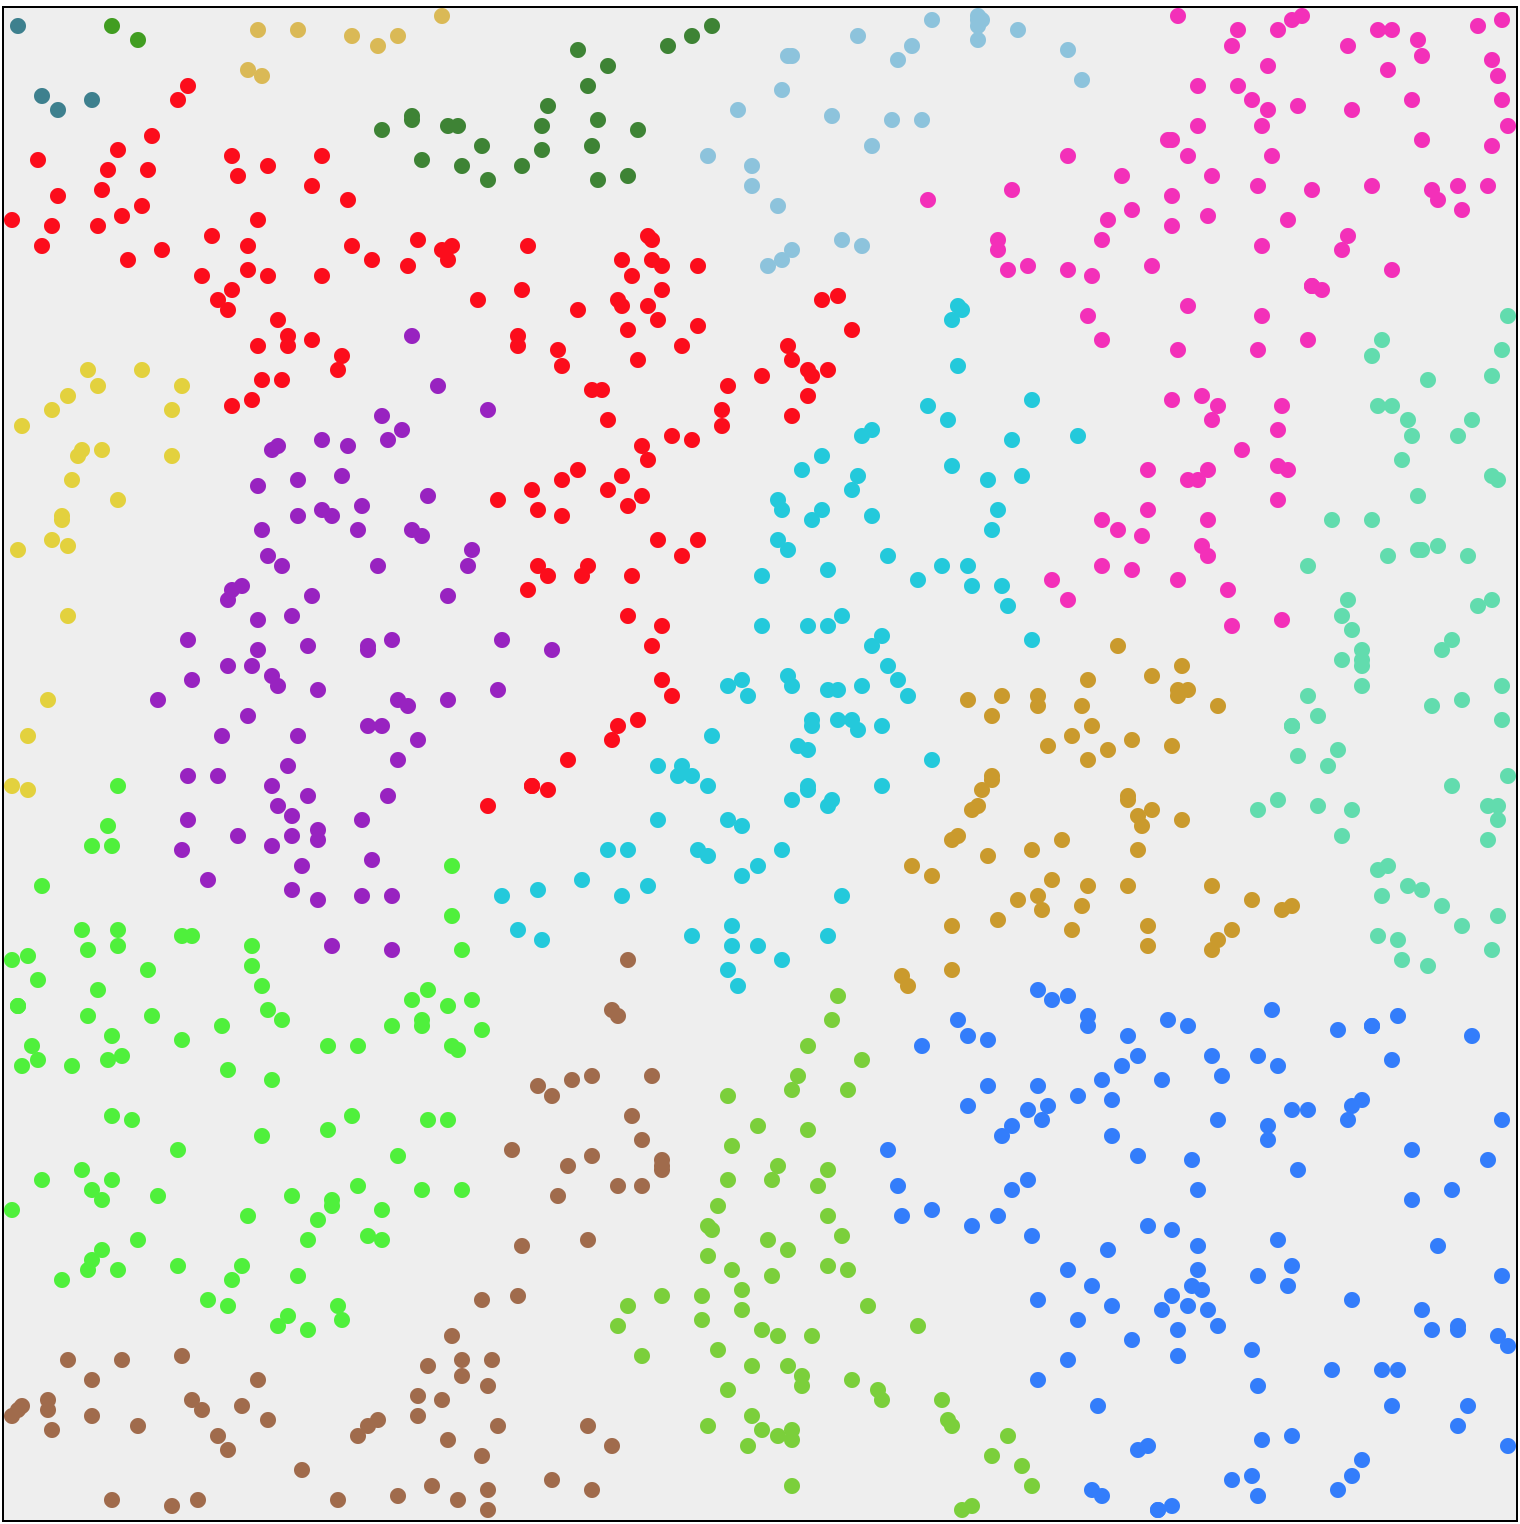
\includegraphics[width=4.5cm]{Images/computations/MINCUT500_500.png} }}%
		\qquad
		\qquad
		\subfloat[Forks]{{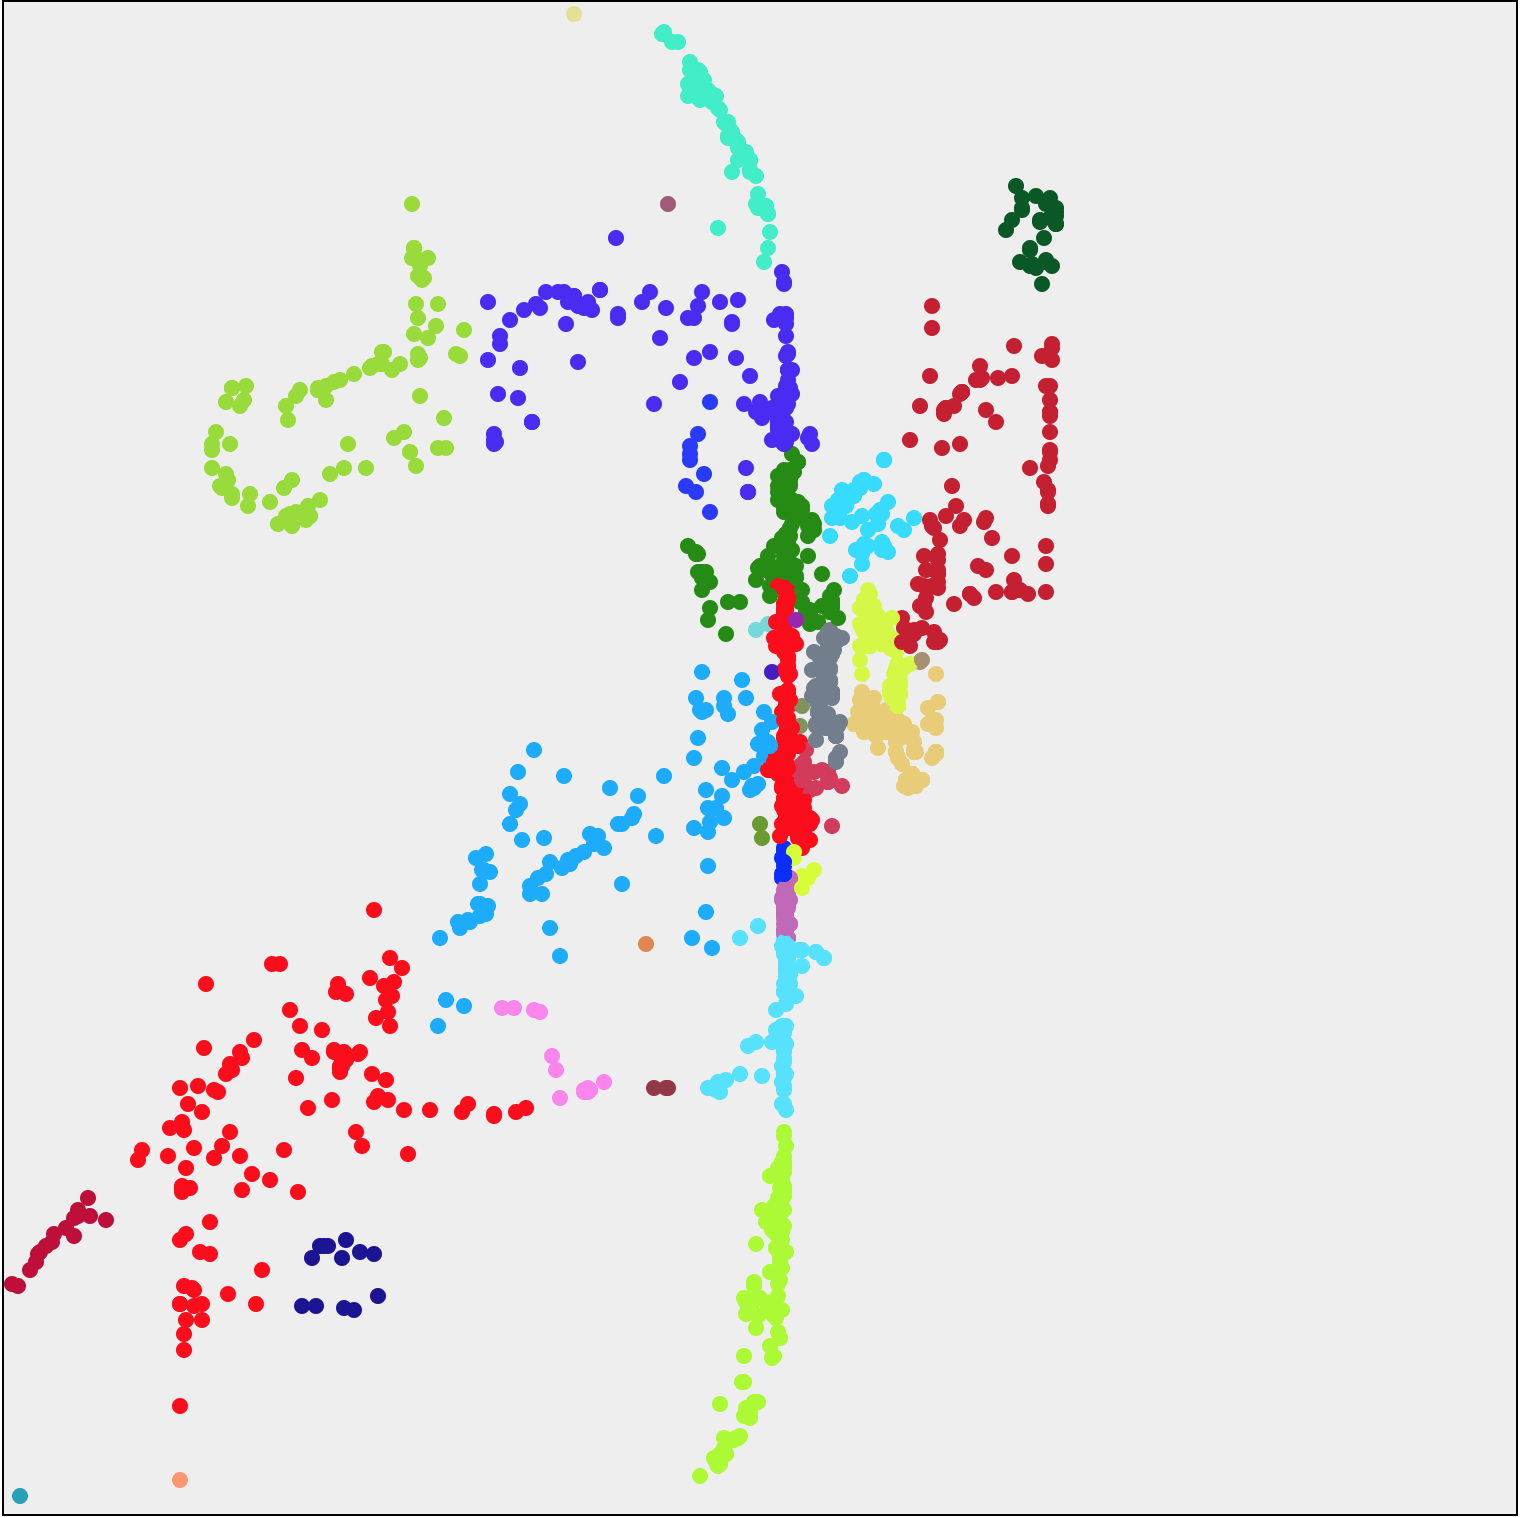
\includegraphics[width=4.5cm]{Images/computations/MINCUT_FORKS.png} }}%

		\subfloat[Lillehammer]{{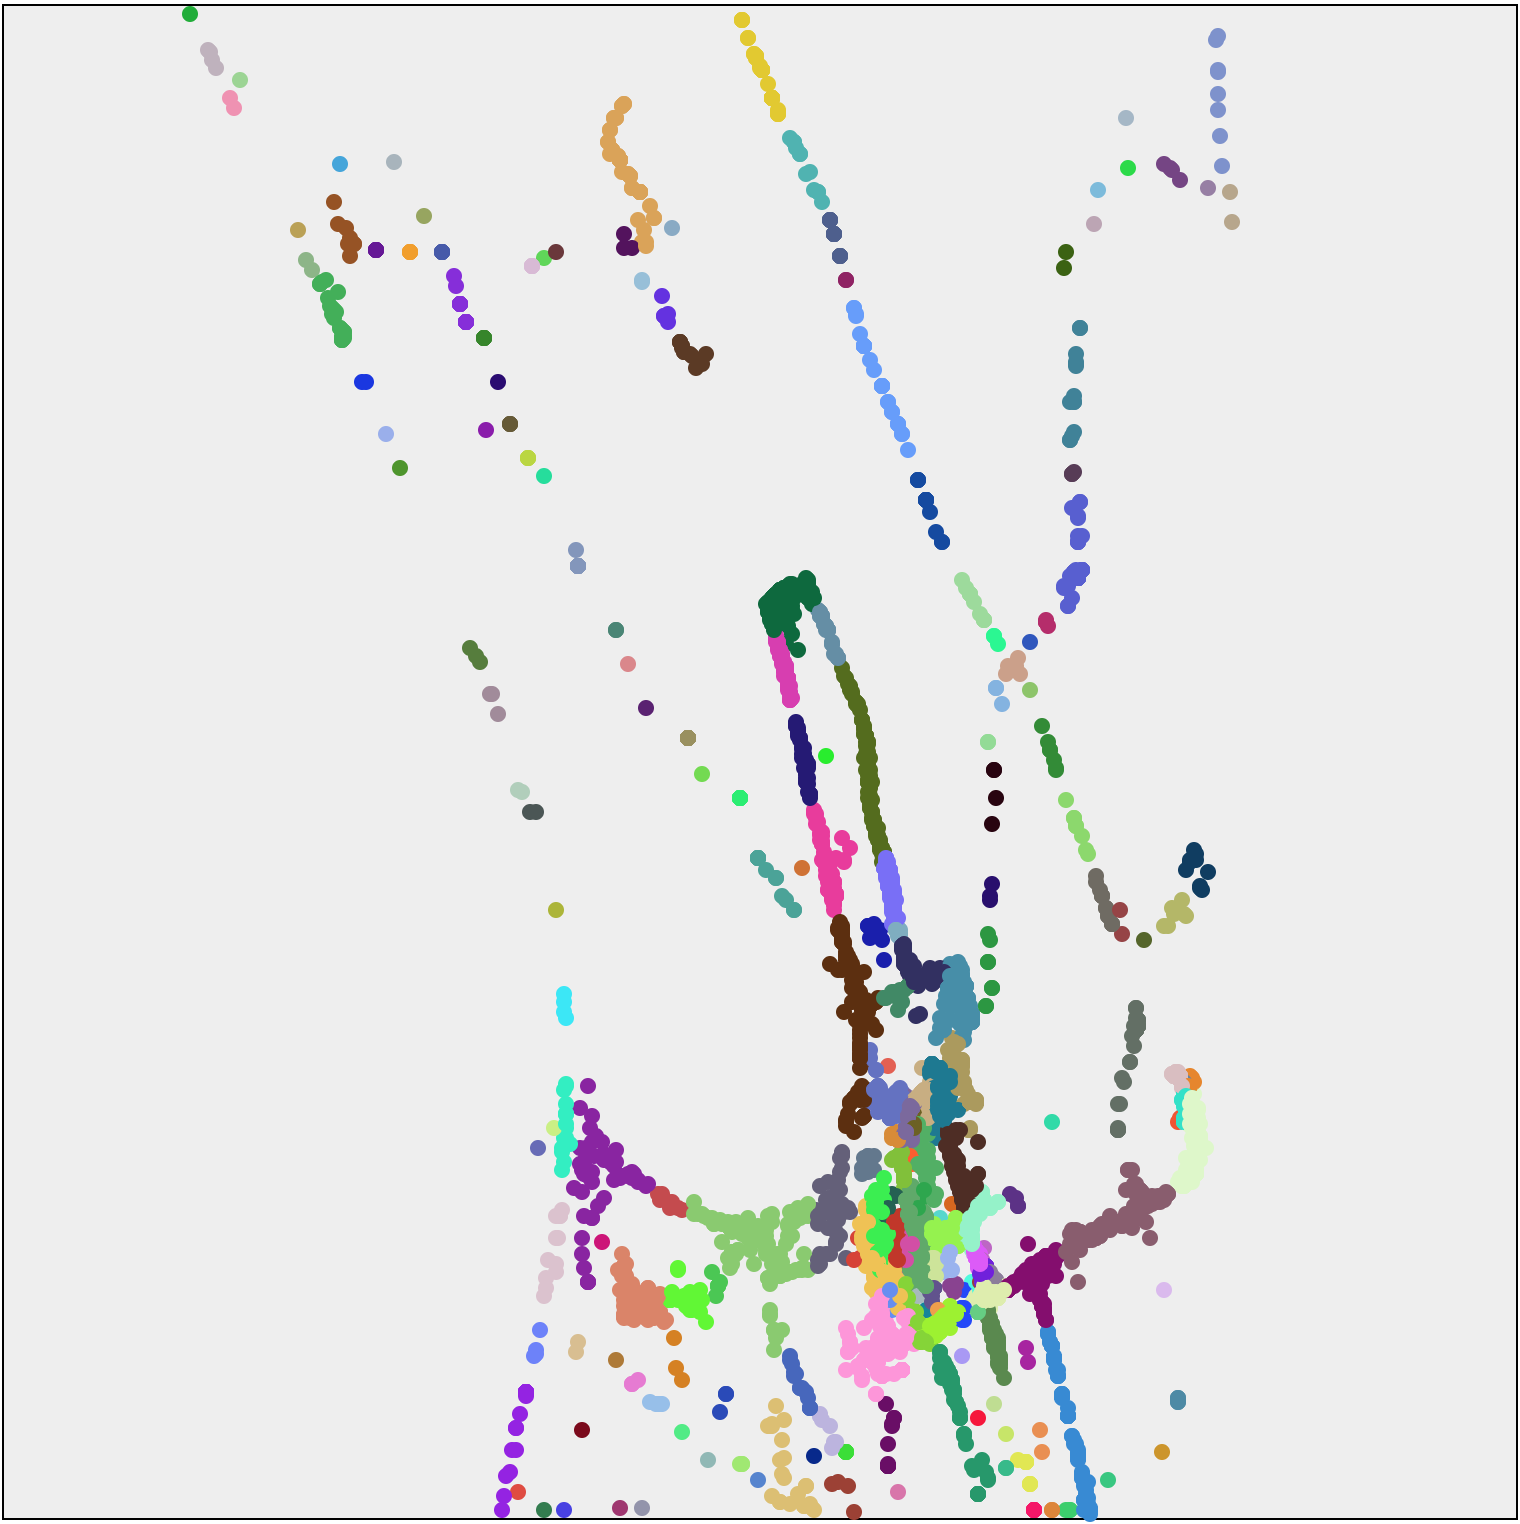
\includegraphics[width=4.5cm]{Images/computations/MINCUT_LILLEHAMMER.png} }}%
		\qquad
		\qquad	
		\subfloat[Tynset]{{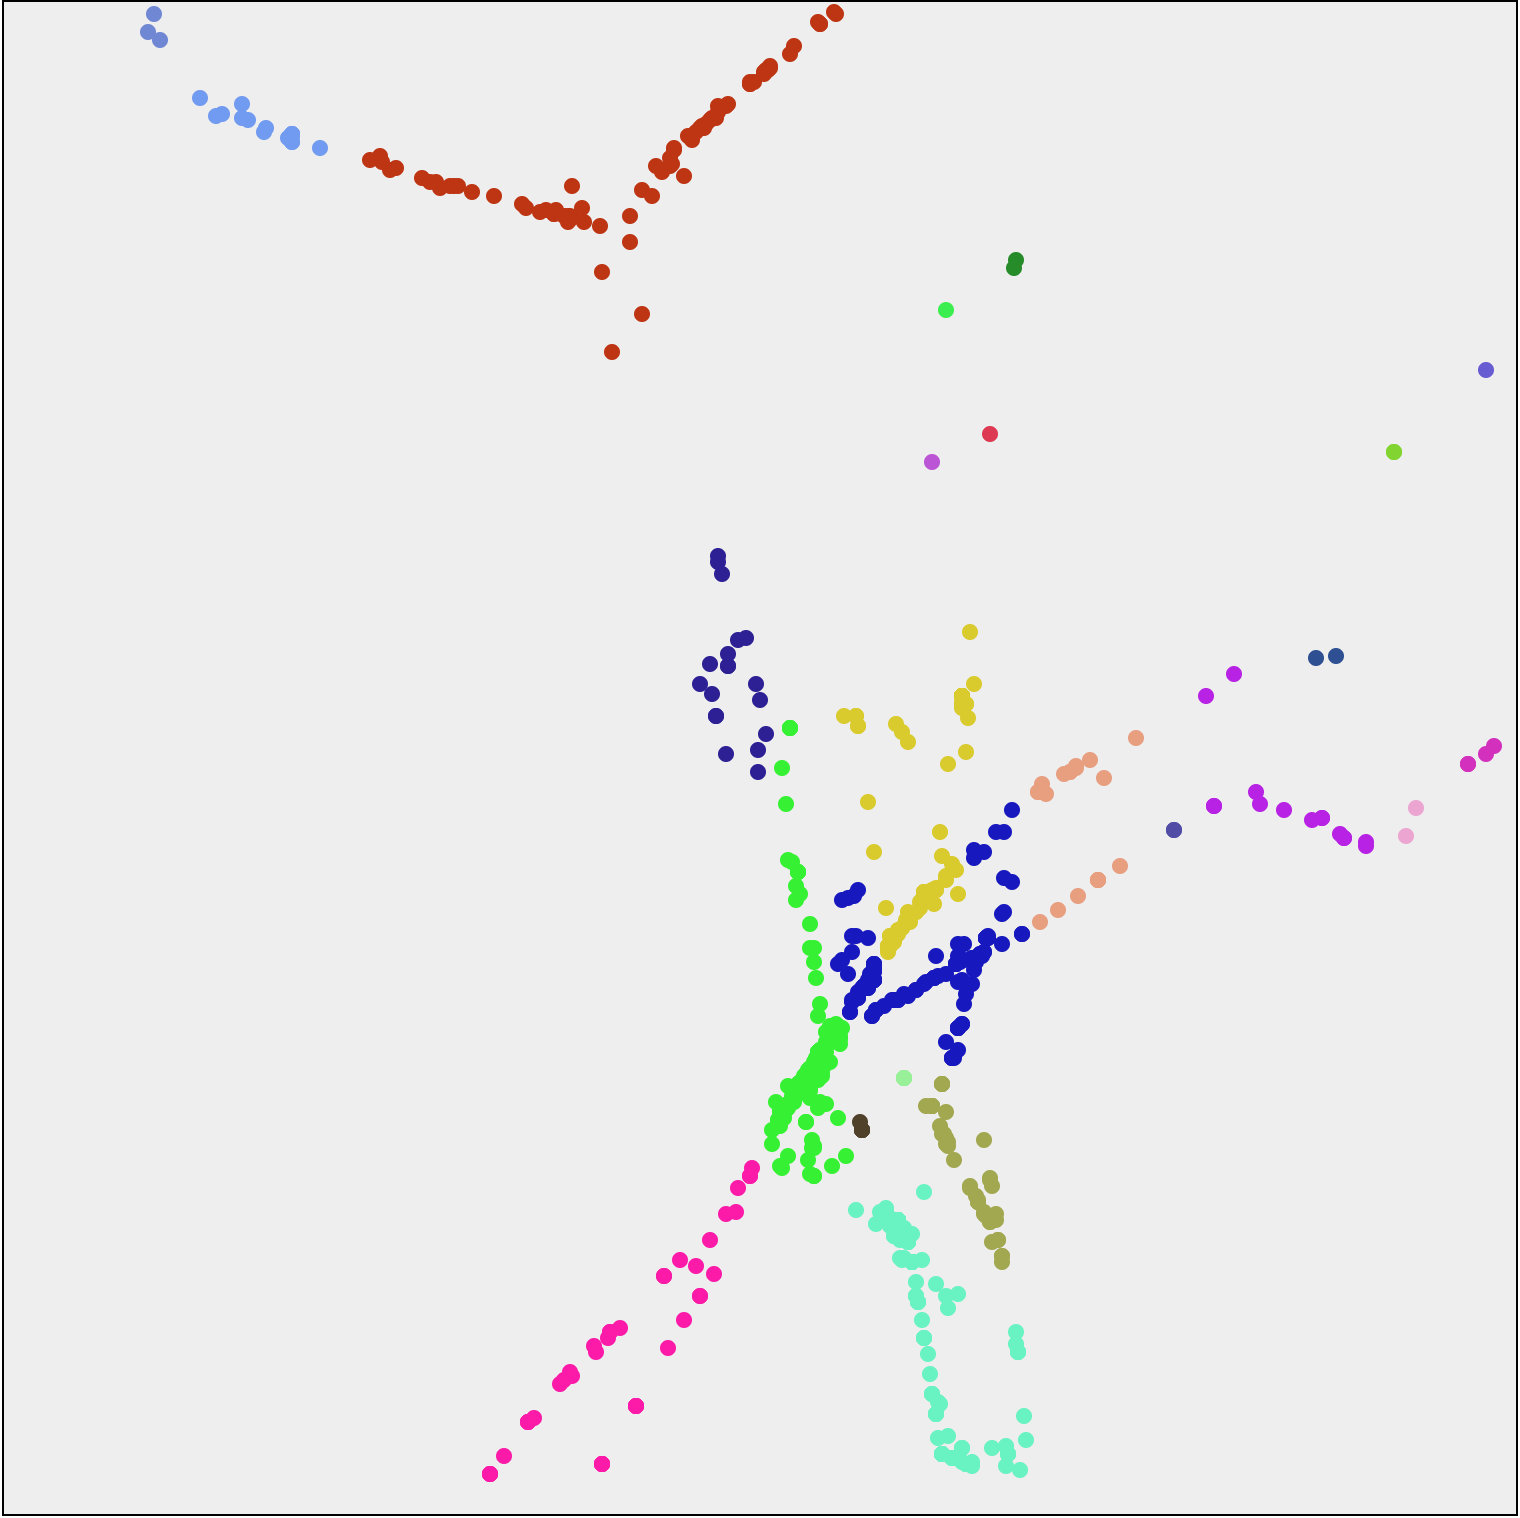
\includegraphics[width=4.5cm]{Images/computations/MINCUT_TYNSET.png} }}%
		\caption{Minimum cut algorithm splitting on different topologies}%
		\label{fig:mincutresults}%
\end{figure}


\subsection{Simulation}
The results of the simulation, using the same four topologies used for previous simulations, with the implementation of minimum cut splitting can be seen in figure \ref{fig:mincutresults} (full scale images can been seen in \ref{appendix:mincutsplitone}). Different groups are distinguished by color, and the group max size is set to 128. 

\subsubsection{Observations}
In the result section of K-means splitting there was a close up examination and comparison of the group division in Tynset's city centre using no splitting and K-means splitting.
In figure \ref{fig:mincutcomparison} a close up of the same area has been made between K-means splitting and minimum cut splitting. The group division seems to 
be very similar, except for a major difference in a cluster on the top left area of the topology (pink color on \ref{fig:mincutcomparison}a).
While the K-means splitting algorithm identifies a neatly separated cluster, the same cluster in the minimum cut method does not include three nodes at the bottom right edge of the cluster.

By looking at the minimum cut, figure \ref{fig:mincutcomparison}b, one can tell that the distance from the three pink nodes to the pink cluster is large.
Actually, it is larger than the distance to the green cluster. The green cluster is far from being the maximum size of 128, so upon a merge it would be reasonable to believe
that a split should happen which would redefine the groups in a better way. This is not happening, and we have to inspect the algorithm we suggested to understand why. 
\begin{figure}
	\centering
		\subfloat[With K-means splitting]{{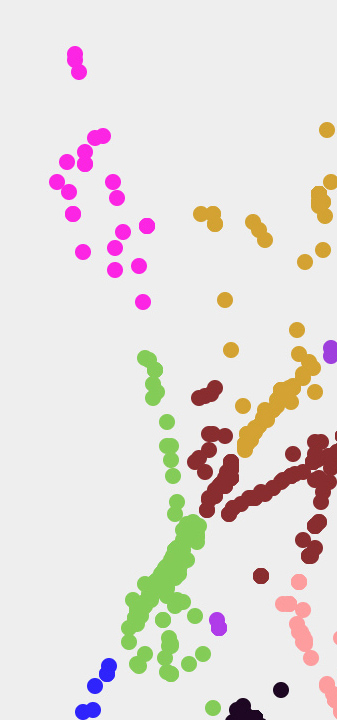
\includegraphics[width=3cm]{Images/computations/TynsetNearKmeans.jpg} }}%
		\qquad
		\subfloat[With minimum cut splitting]{{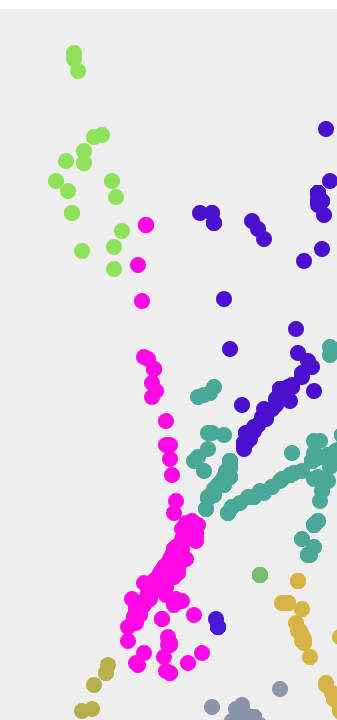
\includegraphics[width=3cm]{Images/computations/TynsetNearMincut.jpg} }}%
		\caption{Comparison between K-means splitting and minimum cut splitting on Tynset}%
		\label{fig:mincutcomparison}%
\end{figure}


\subsubsection{Minimum cut version 2}
The application we created earlier to step through each iteration of the algorithm can help illuminate the problem. The entire solution converges in 11 iterations, but iteration 8 and 9 seems to be the iterations which specifically impacts the result of the cluster in question.
These are illustrated in figure \ref{fig:mincutbug}. In \ref{fig:mincutbug}a, the green group seeks to merge with the pink. They lie very close with a signal strength between them being -45 dBi.
During the split several nodes are kicked out, which can be seen in \ref{fig:mincutbug}b. As expected, the three nodes in question have not been kicked out. By watching the figure it is easier to understand why.
These 3 nodes are obviously less tighter connected than -45dbi, which would the threshold for minimum cuts over this graph, but they are not kicked out because sometime during the split the size of the group becomes lower than the max size of $128$ - before they have the chance to be thrown out. The merge is then immediately accepted. 

An improvement to the algorithm could be to change step 6, so that the minimum cut partitioning would run until no more nodes could be kicked out, even if the group size reached a tolerable size before that. This change would prevent nodes from being left in a group when their closest neighbours have been kicked out, and they would be better off in another group.

\subsubsection{Simulations after re-evaluation}
The final comparison between K-means and the new minimum cut can be seen in figure \ref{fig:mincutbug}. For the full size version of
all four topologies on this simulation as well, see appendix \ref{appendix:mincutsplittwo}. 

\begin{figure}[h]
	\centering
		\subfloat[Iteration 8: The green group seeks to merge with the pink, the signal strength between them for instance being -45dBi]{{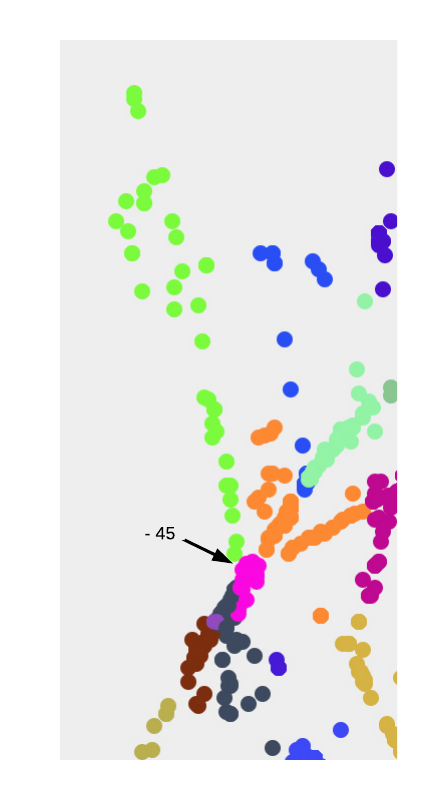
\includegraphics[width=4cm]{Images/mincutbug1.png} }}%
		\qquad
		\subfloat[Iteration 9: After the minimum cut split, some nodes have been thrown out to allow for the merge]{{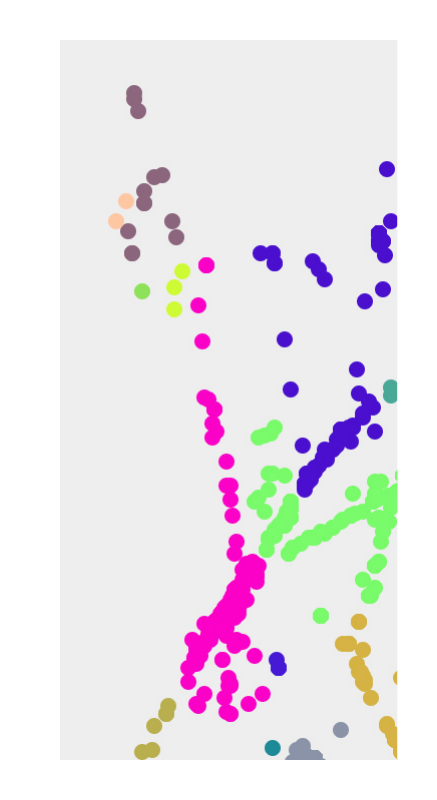
\includegraphics[width=4cm]{Images/mincutbug2.png} }}%
		\caption{Illustrating two algorithm iterations to find the problem source of the minimum cut}%
		\label{fig:mincutbug}%
\end{figure}


\subsection{Observations}
While being slightly more complex to implement in a simulation than the K-means splitting, the results are more reliable and less dependent 
on initial group selection. In a real-world implementation scenario, minimum cut would only need link weights between nodes to work.
Thus while K-means would be hard to realize, the minimum cut method should in theory be little different from simulation to real world implementation, which can be considered
a major benefit. 

\section{Assessment}
In this chapter three clustering methods has been simulated: K-Closest Neighbour Clustering (KCN), KCN Clustering with K-means splitting
and KCN Clustering with minimum cut splitting. This section is dedicated to the evaluation of the results done throughout this chapter, with regards to cluster quality and simulation weaknesses.

\subsection{Result analysis}

\subsubsection{Davies-Bouldin Index}
\label{chap:bouldin}

The Davies-Bouldin Index \cite{Bouldin} is an internal cluster analysis formula. The less scattered a cluster is the lower value is produces, hence a lower Davies-Bouldin Index is desirable.

The formula for the topology wide cluster similarity is as follows:
\[
	DB_\text{topo} = \frac{1}{N}\sum_{i=1}^{N} R_i
\]	
where N = the number of clusters, and $R_i$ is defined as: 

\[
	R_i= \max R_\text{ij} 
\]	

where $i \neq j$ and $R_\text{ij}$ is defined as: 

\[
	R_\text{ij}= \frac{S_i + S_j}{M_\text{ij}} 
\]	

$S$ is the average distance between all points in the cluster, and M is the distance between the centroids of the two clusters $i$ and $j$.

To analyse the clusters we implemented the Davies-Bouldin index. The code for it can be found on GitHub \footnote{\url{https://github.com/hansjny/GroupSimulations/blob/master/Analysis.py}}.
The result of the Bouldin-Index analysis can be seen in figure \ref{fig:bouldin}.
\begin{figure}[h]
	\centering
		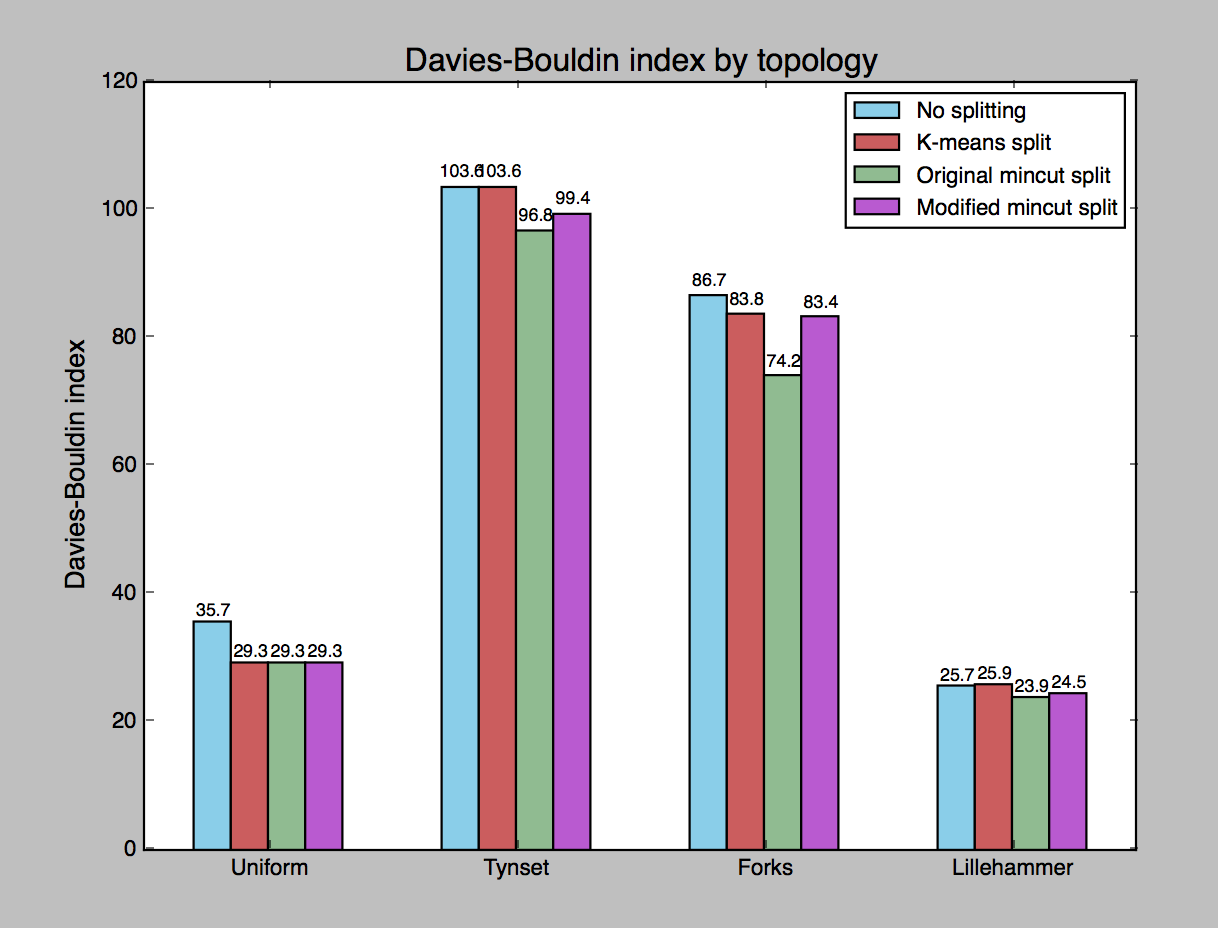
\includegraphics[width=14cm]{Images/Bouldin.png}
		\caption{Bouldin-Index of all simulations}%
		\label{fig:bouldin}%
\end{figure}

\subsection{Simulation weaknesses and data bias}
This subsection will consider all the different aspects that has not been considered
when producing the simulated results, but might have an impact in a real life implementation. 

\subsubsection{Volatility} 
All the simulations take a static network topology as an input. The static topology is an image of a network topology in a given state, and is not representative
of the volatile nature of modern networks. Actually, it is more like a computation than a simulation in its rightful meaning.
While it is true that most access points are relatively stationary and constant, it is increasingly popular to create ad-hoc on-demand Wi-Fi
networks using cell phones or using computers as access points. Additionally resetting of routers, power outages, etc. means that access points come and go. 
Hence it is indisputable that network topologies are volatile, and the group clustering algorithm should, when final, run as a continuous operation. 
Any reader of this thesis will know that ways the algorithm can handle volatility has been considered, enabled by group splitting,
but the simulation framework does not support inserting or removing nodes during the computation, hence only static environments that quickly converges have been tested. 

\subsubsection{Signal strength reporting bias}
The group computations have been based on the signal strength of all nearby access points, and the $dBi$ values that denotes all signal strengths have been calculated using the
free space path loss formula. As distance is the only variable that affects the result of the signal strength calculation,
it means that the signal strength levels becomes a symmetric binary relation between nodes. In the real world this is not the case, and also the reason agglomerative clustering was deemed
less ideal. Access points may interfere with each other differently, and the signal strength values may change when there are variations in the environment. This is the reasons deadlocks could
occur if implementing regular agglomerative hierarchical clustering and the motivation behind creating K-Closest Neighbour Clustering, even though the topologies used in this thesis actually
could work well with agglomerative clustering. We have no simulations of how groups would look if the perceived signal strength between two nodes were not mutual.

\subsubsection{Dimensionality and node location reporting bias} 
Both the data that has been randomly generated, and the data fetched from \verb|wigle.net| takes the $x$ and $y$ axes in account. Obtaining data in three dimensions is harder.
WiGLE places the access points using longitude and latitude as all their data is acquired using ground-level trilateration. 
By creating clusters based on information in two dimensions there is no way to know how the algorithm behaves in a 3-dimensional world. Of course, it is reasonable to think that an algorithm
which is based on distance in two dimensions should also work well in three dimensions, but there have been done no simulations in three dimensions.
As mentioned in the data-mining chapter, WiGLE has a tendency to place nodes closer to roads, which means that the positioning of nodes may not be strictly accurate in two dimensions either.  


\subsection{Summary and discussion}
Before beginning the work on this chapter it was hard to envision how groups could be formed in a distributed manner, without any central controller having a top down view of
the landscape of wireless access points. While many questions still remain, some have also been answered. 

The small modification to the agglomerative clustering algorithm which we called KCN Clustering yielded promising cluster topologies already.
This algorithm could provide a natural starting point for a real-world implementation in a static network topology.
However, this algorithm alone does not handle changes in the network environment very well, as once a group's maximum size is reached, it can not be modified. 
Hence, we not recommend this to be used for any final implementations, but still it could possibly provide useful for testing scenarios, possibly in an early
implementation when a distributed channel allocation algorithm is to be tested across the group.

It deserves mentioning that agglomerative clustering could have been used with the assumption that all signal strength observations was a symmetric relation.
This was not done to reduce the amount of assumptions. Not making the assumption does arguably represents a more realistic scenario. 

To extend this type of clustering to work in a dynamic environment, the notion of splitting was introduced, and tested through the methods of K-means and minimum cut.

K-means was an interesting clustering algorithm to work with. The promising splitting results observed on the simulation topologies was especially fun to see, as
the K-means method was adapted to fit the clustering purpose, and not implemented as a textbook K-means clustering.
i
However, when comparing the K-means and the minimum cut algorithm to decide which one is the best bet for a real-world implementation of a splitting algorithm,
the minimum cut algorithm comes off as the easiest to implement given the limited knowledge of the surrounding nodes each access point has access to.
Most importantly, the minimum cut implementation conforms to all requirements postulated in \ref{chap:requirements}, except requirement 4. By studying the
final topologies it is clear that there is still room for further optimization.

The interesting results from the Davies-Bouldin from \ref{chap:bouldin} analysis is that it shows that the modified version of the minimum cut algorithm performs less well than the original one.  
But as we saw earlier, the original version of the minimum cut algorithm produces results that are undesirable. Most likely, this means that the results
of the modified version of minimum cut produces clusters that are more scattered. So maybe the modification to it was unnecessary, it all depends on how one wants
to define the quality of a cluster. Even so, this confirms that the evaluation of clusters can be just as hard as the clustering task itself as indicated by Darius Pfitzner et al. in \cite{fitzner}.



%\subsection{Uniformly distributed nodes}
%We will look at how groups were created in different topology scenarios. 
%All topologies presented in this section was created by the topology generation program,
%but with different input parameters. Groups are distinguished by node color, where nodes
%of the same color represents members of the same group. 
%%\subsubsection{Scenario 1}
%Computed with 200 nodes with a maximum of 128 members in each group.
%
%As can be seen in figure \ref{fig:200_128} the algorithm divides the nodes in two
%sections. For clarity, a divisive line has been drawn around each group,
%in case colors are not available.
%When two major groups merged, the biggest groups surpasssed 128 members and began
%kicking out members. The excess members formed the black group at the bottom. 
%
%\begin{figure}
%\center
%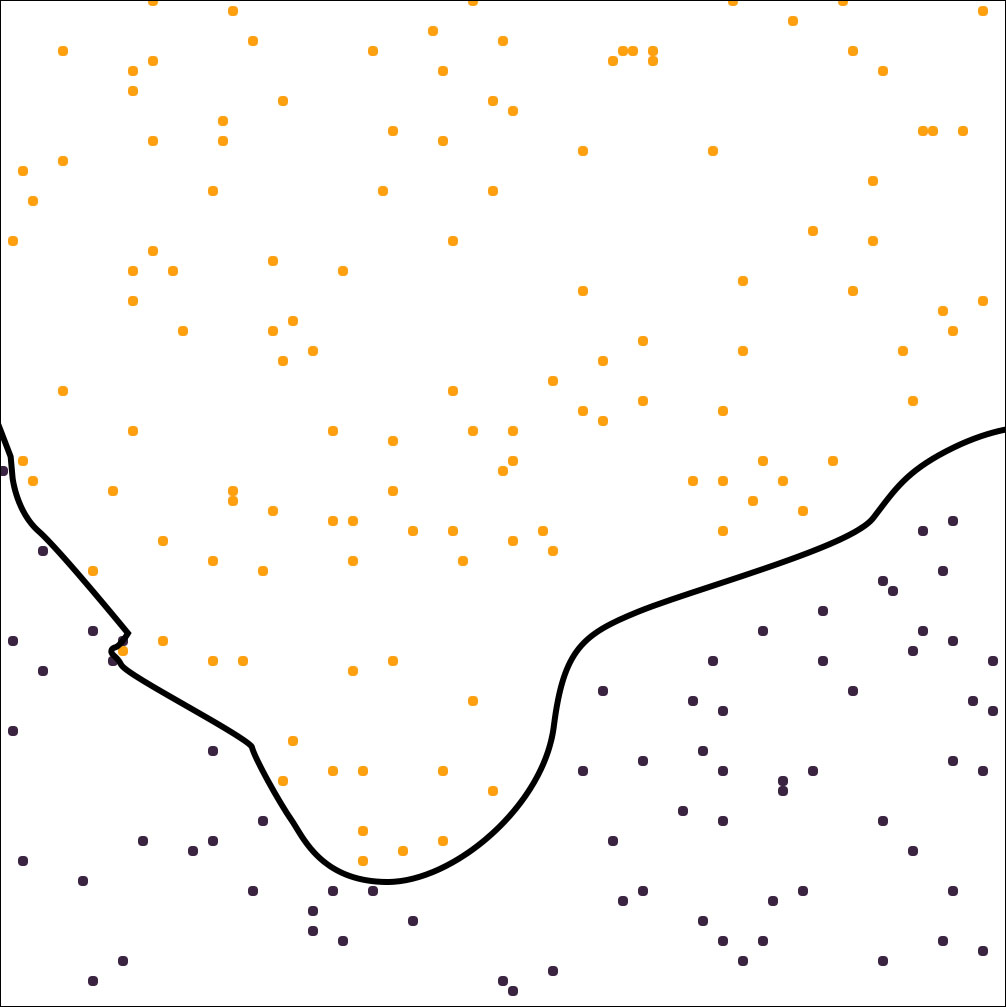
\includegraphics[scale=0.45]{Images/grouptest_1.jpg}
%\caption{200 nodes, $memberThresh=128$, $size=200x200$
%\label{fig:200_128}
%\end{figure}
%
%
%\subsubsection{Scenario 2} \label{scen2}
%Computed with 200 nodes with a maximum of 10 members in each group.
%
%The result of this computation, seen in figure \ref{fig:200_10}, is a little less obvious.
%The groups are again distinguished by different color, but for clarity we add a gray connecting
%blob for nodes in the same group. Also blobs connected with a line are in the same group. 
%
%It is worthy to take notice that one group is especially scattered around the graph.
%At first eyesight, it looks like an algorithm deficiency, but the reason is quite simple:
%when nodes are kicked out of a group during a merge, they will connet to other nodes
%that belong in a group where $n$ has not yet reached $memberThresh$. When this have happened a couple of times, everyone has found a group except for the remaining few.
%These are typically straggler nodes or smaller clusters separated from the others.
%They are not big enough to reach the group $memberThresh$ on their own, so the merge with other
%nodes that are in unmaxed groups. Thus, even though they have neighbours which
%influence them more, they can only merge with nodes further away,
%because that is the only unlocked group that remains.
%\begin{figure}
%\center
%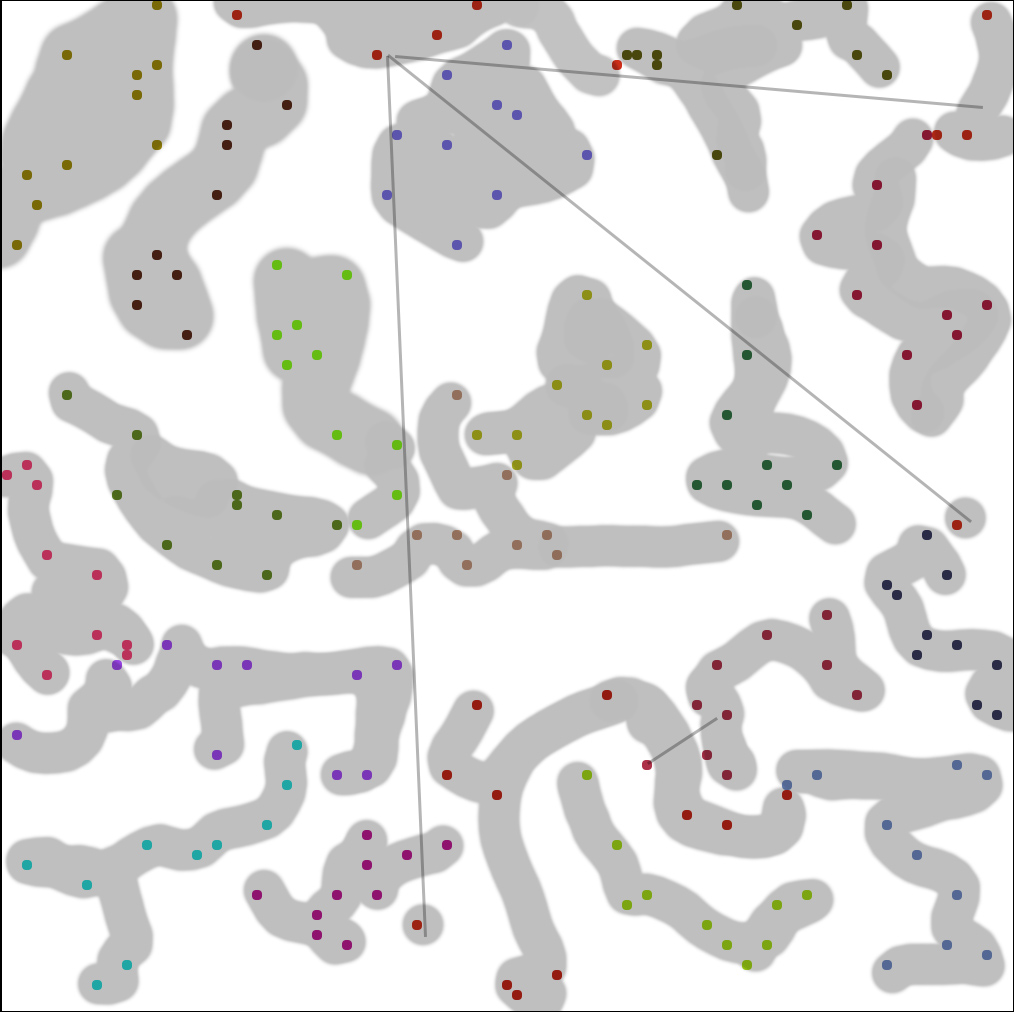
\includegraphics[scale=0.45]{Images/grouptest_2.jpg}
%\caption{200 nodes, $memberThresh=10$, $size=200x200$}
%\label{fig:200_10}
%\end{figure}
%
%\subsubsection{Scenario 3}
%Computed with 5000 nodes, with a maximum for 64 members in each group. 
%
%Figure \ref{fig:2000_64} shows the result of the computation. Because of the quantity
%of nodes and the clear separation of groups, they are easily distinguished by color.
%This topology is much denser than the others, and can vaguely resemble the density of highly populated areas.
%
%We can clearly see that the overall tendency is that groups are formed
%in concentrated areas of nodes. However, some groups are scattered, sometimes
%all over the map. An example of a scattered group is highlighted
%in figure \ref{fig:2000_64}. Its  member nodes has a thicker black line around them. 
%\begin{figure}
%\center
%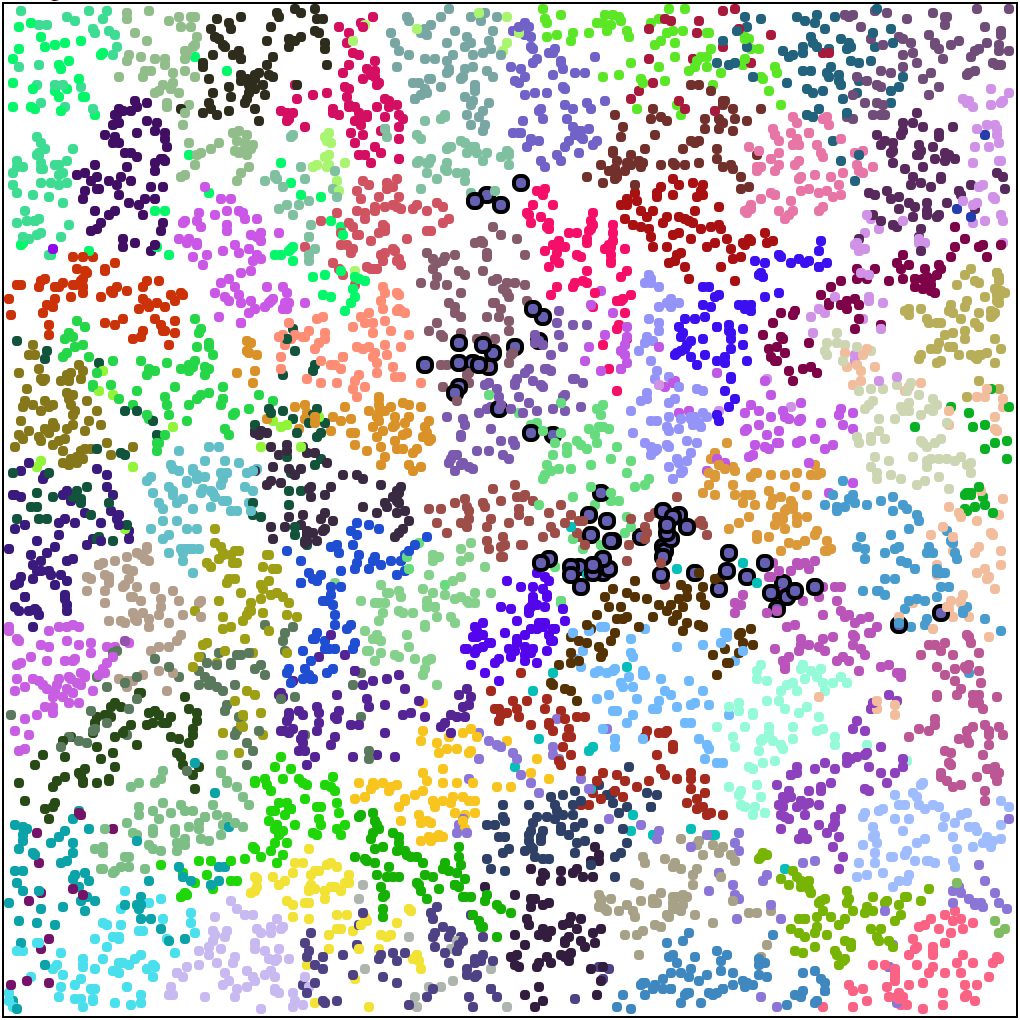
\includegraphics[scale=0.45]{Images/scenario3alt.png}
%\caption{5000 nodes, $memberThresh=64$, $size=2000x2000$}
%\label{fig:2000_64}
%\end{figure}






%
%\begin{figure}
%\centering
%\begin{minipage}{.6\textwidth}
%	\center
%	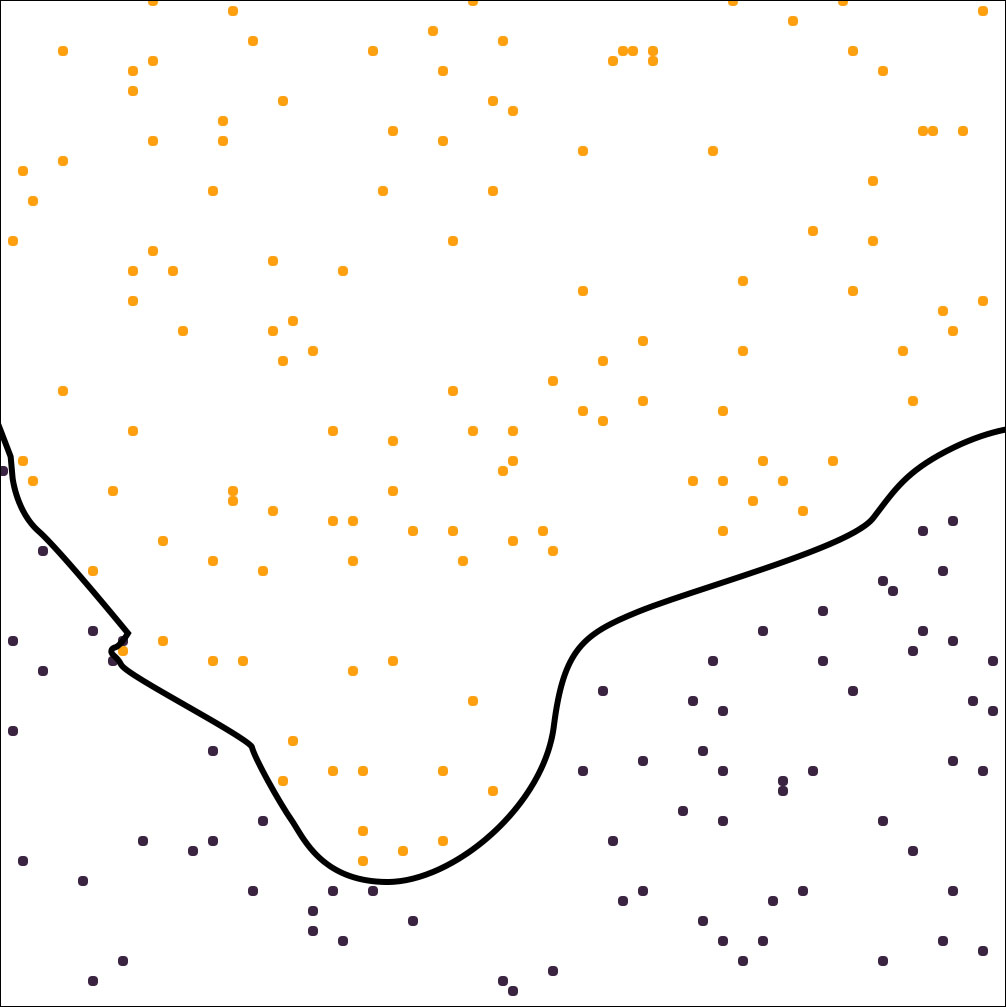
\includegraphics[width=0.9\linewidth]{Images/grouptest_1.jpg}
%	\captionof{figure}{\newline200 nodes, $memberThresh=128$}
%	\label{fig:200_128}
%\end{minipage}%
%\begin{minipage}{.6\textwidth}
%	\center
%	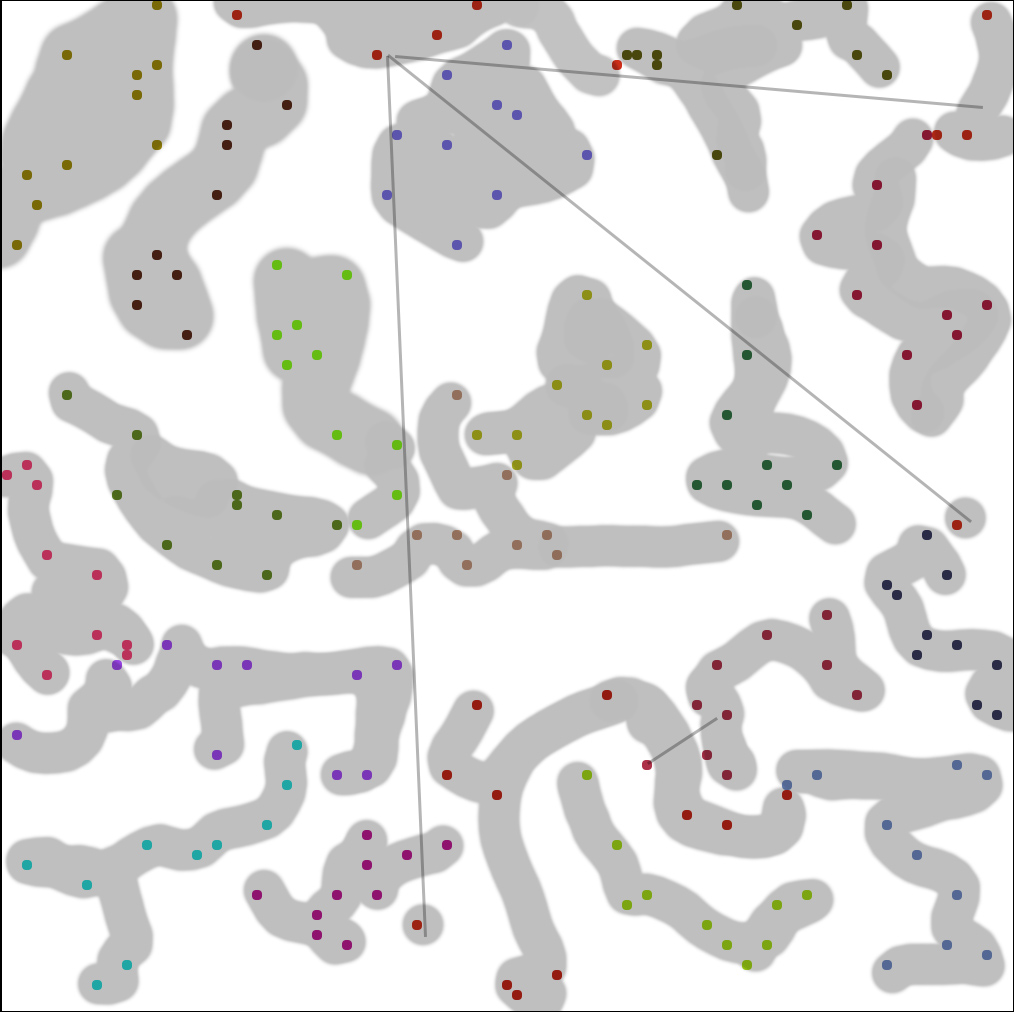
\includegraphics[width=0.9\linewidth]{Images/grouptest_2.jpg}
%	\captionof{figure}{Another figure}
%	\label{fig:test2}
%\end{minipage}
%\end{figure}



%
%\section{Results}
%By running the scripts that parses data from Wigle on populated areas, we should get an idea 
%on how the algorithm performs in more realistic topologies. We will have a look at three
%scenarios where the group allocation data is based on AP-data. 
%
%Three suitable locations has been selected to perform the testing on Lillehammer (Norway)
%a smaller city, Tynset (Norway) a less densely populated area, 
%and Forks (Washington, United States). All tests were 
%ran with a maximum group size of 128, and a $-dBi$ threshold of $-80$. 
%
%\subsubsection{Lillehammer}
%\begin{figure}
%\center
%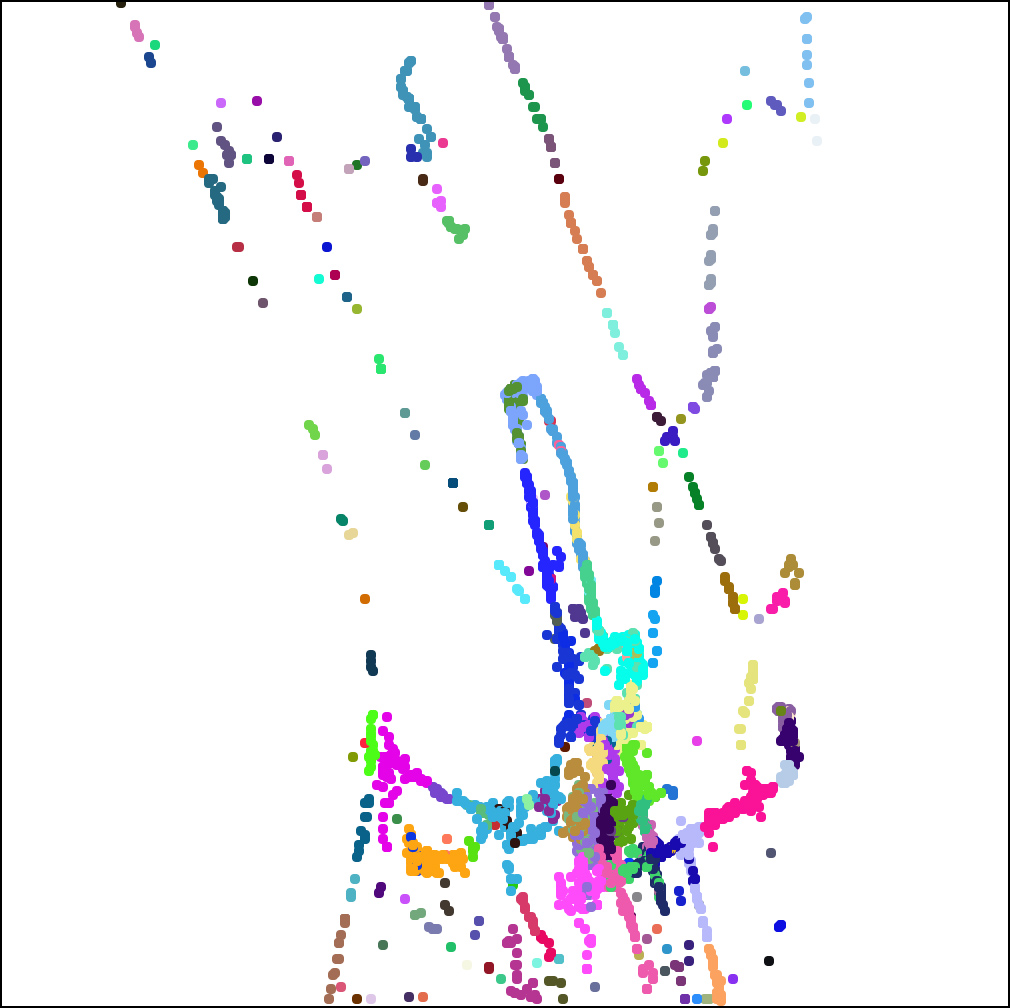
\includegraphics[scale=0.46]{Images/cities/lillehammer_groups.jpg}
%\caption{Lillehammer}
%\label{fig:lillehammer_topo}
%\end{figure}
%
%The computation results of Lillehammer can be seen in figure \ref{fig:lillehammer_topo}.
%The topology is of medium density, consisting of 4990 APs, and is 2572 meters high 
%and 8418 meters wide. From the tight clusters in the middle it is easy to make out the city centre.
%We can clearly see different groups with different sizes. Some of the smallest groups
%are highly likely so small because the distance to other nodes is too high for
%the group to hear. In the denser areas they are occasionally very
%entangeled, and it can be hard to make out the group borders.
%
%Another thing to notice is that APs are nearly always placed in straight lines.
%The straight lines are roads, and as Wigle collects data based on triangulation, the nodes
%that is only seen once will get the position they are observed in, and not an actual
%triangulated position. 
%\subsubsection{Tynset}
%The computation results of Tynset can be seen in figure \ref{fig:tynset_topo}. 
%The topology consists of 726 APs, is 1670 meters high and  6720 meters wide. 
%Unsurprisingly it resembles Lillehammer on a smaller scale.
%Again we see
%some very clearly defined groups, but in the city centre there are groups
%which overlaps. We can also see nodes that are alone in their group,
%because they are too far away from anyone else.
%Much like Lillehammer, this topology is also strongly affected by the weak
%
%triangulation of the APs, so most APs seems to be placed on top of a road. 
%
%\begin{figure}
%\center
%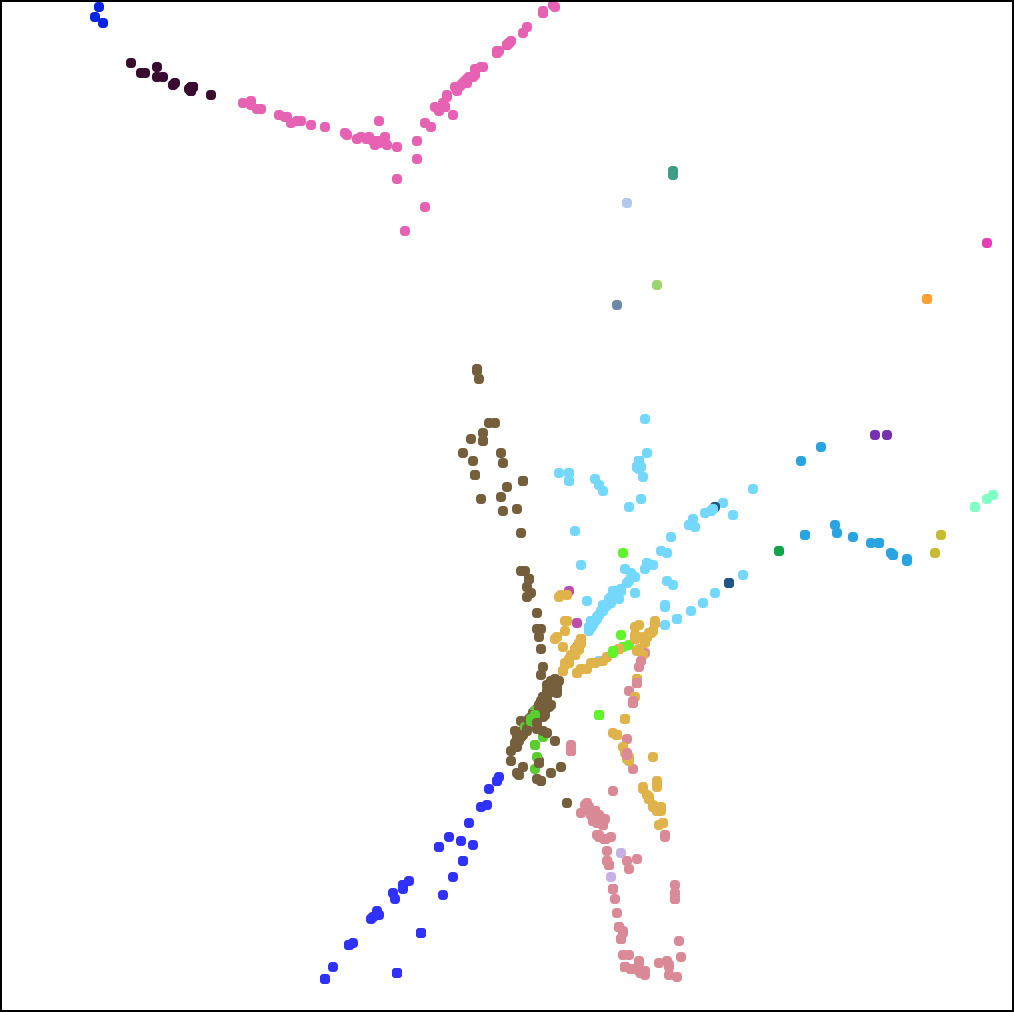
\includegraphics[scale=0.46]{Images/cities/tynset_groups.jpg}
%\caption{Tynset}
%\label{fig:tynset_topo}
%\end{figure}
%
%\subsubsection{Forks}
%
%The computation results of Forks can be seen in figure \ref{fig:forks_topo}. 
%The topology consists of 1715 nodes, and is 2122 meters high and 4495 meters wide. It
%is important to include, because it is quite different from the other topologies and
%represents a variation from the typical town and city structure of Norway.
%The size of the groups are a little more uniform when comparing it to the others.
%This can explained by the the smaller area the town is contained within. When a group
%is not full, it will almost always hear someone that it can merge with.
%We still have groups overlapping each other in the denser regions in Forks as well. 
%What is worth noticing is that the APs are positioned more realistically as locations
%of households. American towns looks more like a grid with roads in between households,
%which makes triangulation easy and a lot more accurate. 
%
%\begin{figure}
%\center
%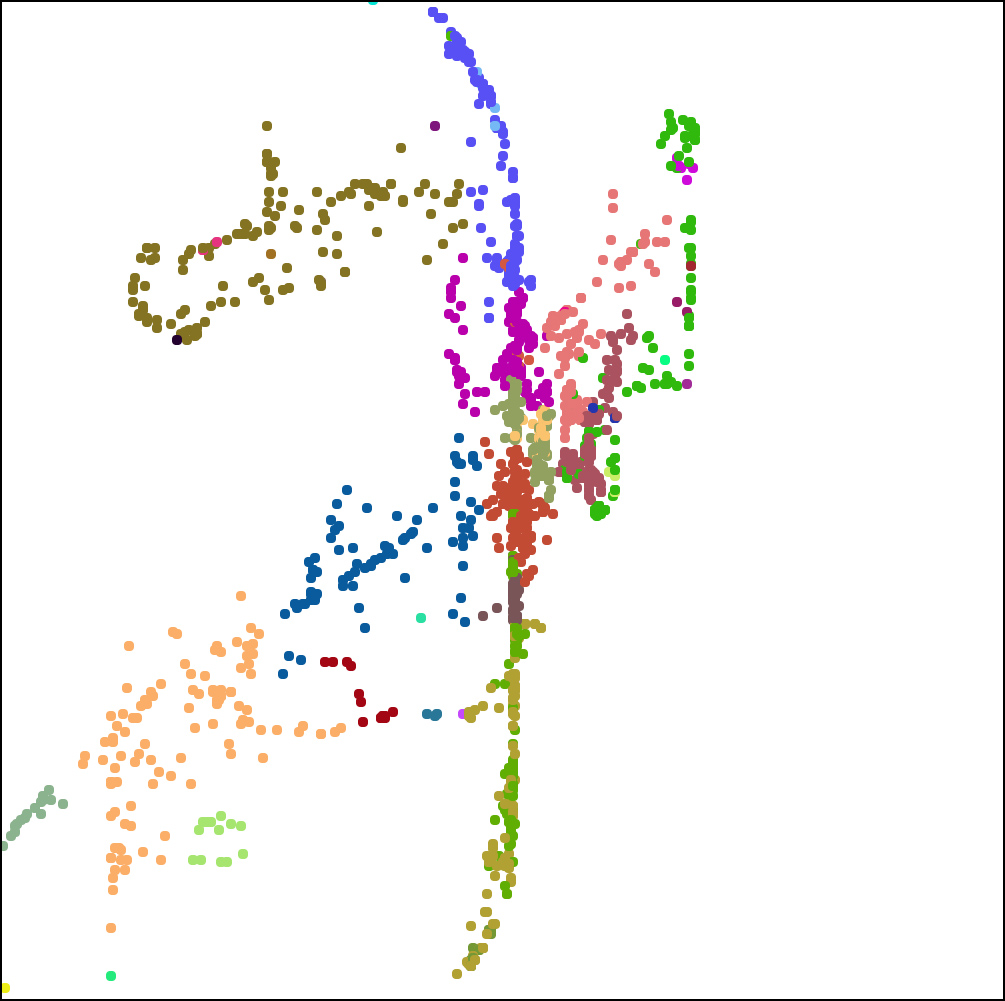
\includegraphics[scale=0.46]{Images/cities/forks_groups.jpg}
%\caption{Forks}
%\label{fig:forks_topo}
%\end{figure}
%
%
%
%

\chapter{Future Work}
\section{ResFi}
\section{Raft}




%
%\makeatletter
%\def\BState{\State\hskip-\ALG@thistlm}
%\makeatother
%\subsection{Pseudocode}
%\begin{algorithm}
	%\caption{Connected group}\label{congroup}
	%\begin{algorithmic}[1]
	%\Procedure{MergeGroup}{}
	%		\State $\textit{members} \gets \text{1}$
	%		\State $i \gets \textit{patlen}$
	%		\If {$i > \textit{stringlen}$} \Return false
	%		\EndIf
	%		\State $j \gets \textit{patlen}$
%			\If {$\textit{string}(i) = \textit{path}(j)$}
%			\State $j \gets j-1$.
%			\State $i \gets i-1$.
%			\EndIf
%			\State $i \gets i+\max(\textit{delta}_1(\textit{string}(i)),\textit{delta}_2(j))$.
%			\State \textbf{goto} \emph{top}.
%		\EndProcedure
%	\end{algorithmic}
%\end{algorithm}


\backmatter
\printbibliography
\end{document}
